\chapter{Analisis}
\label{chap:analisis}

\section{Tingkat Kepatuhan BlueTape Terhadap \textit{WCAG} 2.1}
\label{sec:kepatuhan_bluetape_terhadap_wcag_2.1}
Pada subbab ini berisi hasil analisis atas sukses atau tidaknya aplikasi BlueTape dalam mematuhi tujuh puluh delapan poin kriteria sukses yang terdapat dalam \textit{WCAG} 2.1. Pembahasan setiap poin kriteria sukses dikelompokkan ke dalam subbab-subbab sesuai masing-masing kategori kriteria sukses. Pada subbab-subbab berikutnya menjelaskan alasan mengapa bagian-bagian tersebut dinilai patuh atau tidak patuh.

\subsection{\textit{Perceivable}}
\label{subsec:kepatuhan_bluetape_perceivable}
Pada subbab ini dibahas kriteria-kriteria sukses yang termasuk ke dalam kategori \textit{perceivable}. Hasil sukses atau tidaknya aplikasi BlueTape terhadap poin-poin kriteria sukses dalam kategori ini ditampilkan pada Tabel \ref{tab:kepatuhan_bluetape_perceivable}.

\begin{table}[H]
    \centering 
    \caption{Kepatuhan BlueTape terhadap prinsip \textit{Perceivable}}
    \label{tab:kepatuhan_bluetape_perceivable}
    \begin{tabular}{|c|c|c|}
        \toprule
        Kriteria Sukses & Hasil (sukses/tidak) & Tingkat Kepatuhan \\

        \midrule
        \rowcolor{darkred} 1.1.1 & Tidak Sukses & A \\
        1.2.1 & Sukses & A \\
        1.2.2 & Sukses & A \\
        1.2.3 & Sukses & A \\
        1.2.4 & Sukses & AA \\
        1.2.5 & Sukses & AA \\
        1.2.6 & Sukses & AAA \\
        1.2.7 & Sukses & AAA \\
        1.2.8 & Sukses & AAA \\
        1.2.9 & Sukses & AAA \\
        \rowcolor{darkred} 1.3.1 & Tidak Sukses & A \\
        1.3.2 & Sukses & A \\
        1.3.3 & Sukses & A \\
        1.3.4 & Sukses & AA \\
        \rowcolor{brightred} 1.3.5 & Tidak Sukses & AA \\
        \rowcolor{pink} 1.3.6 & Tidak Sukses & AAA \\
        1.4.1 & Sukses & A \\
        1.4.2 & Sukses & A \\
        \rowcolor{brightred} 1.4.3 & Tidak Sukses & AA \\
        1.4.4 & Sukses & AA \\
        1.4.5 & Sukses & AA \\
        \rowcolor{pink} 1.4.6 & Tidak Sukses & AAA \\
        1.4.7 & Sukses & AAA \\
        \rowcolor{pink} 1.4.8 & Tidak Sukses & AAA \\
        1.4.9 & Sukses & AAA \\
        \rowcolor{brightred} 1.4.10 & Tidak Sukses & AA \\
        1.4.11 & Sukses & AA \\
        1.4.12 & Sukses & AA \\
        1.4.13 & Sukses & AA \\
        
        \bottomrule
        \multicolumn{2}{|c|}{Tingkat kepatuhan tertinggi yang dicapai} & - \\
        \bottomrule

    \end{tabular}
\end{table}

\subsubsection{\textit{Text Alternatives}}
\label{subsubsec:kepatuhan_bluetape_text_alternatives}
Pada subbab ini dibahas alasan mengapa poin kriteria sukses pada kategori \textit{text alternatives} dinilai sukses atau tidak sukses.

\paragraph{Kriteria Sukses 1.1.1 \textit{Non-text Content}}
\label{par:kepatuhan_bluetape_kriteria_sukses_1.1.1}
(Tidak Sukses)\\

Kriteria ini tidak sukses dipatuhi karena pada halaman cetak transkrip, manajemen cetak transkrip, perubahan kuliah, dan manajemen perubahan kuliah terdapat konten berupa ikon yang tidak memiliki nama yang dapat diidentifikasi. Konten-konten ini terletak pada kolom "Aksi". Contoh kesalahan dapat dilihat pada \textit{Listing} \ref{lst:1.1.1_ikon_tanpa_nama}. Contoh tampilan pada halaman web dapat dilihat pada Gambar \ref{fig:1.1.1_non_text_content_2}. Contoh tautan untuk halaman yang bermasalah dapat dilihat di \url{https://bluetape.azurewebsites.net/PerubahanKuliahManage}.
\begin{lstlisting}[frame=single, label={lst:1.1.1_ikon_tanpa_nama}, language=HTML, caption=Pelanggaran Kriteria Sukses 1.1.1 pada Halaman Manajemen Perubahan Kuliah]
    <td>
        <a data-open="detail12">
            <i class="fi-eye"></i>
        </a>
        <a target="_blank" href="/PerubahanKuliahManage/printview/12">
            <i class="fi-print"></i>
        </a>
        <a data-open="konfirmasi12">
            <i class="fi-like"></i>
        </a>  
        <a data-open="tolak12">
            <i class="fi-dislike"></i>
        </a>
        <a data-open="hapus12">
            <i class="fi-trash"></i>
        </a>
    </td>
\end{lstlisting}

\begin{figure}[H]
    \centering  
    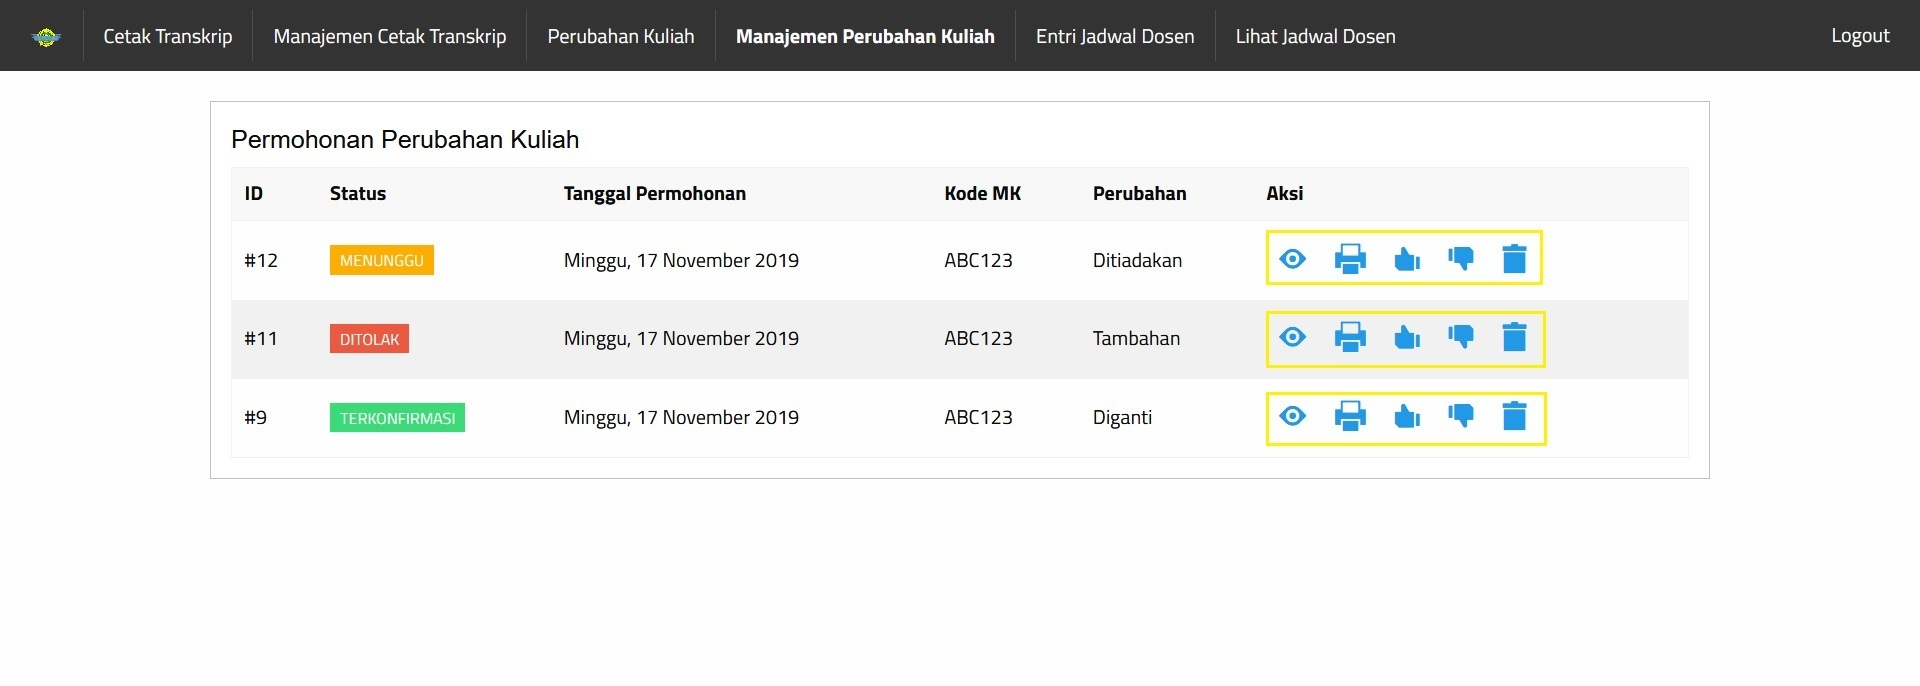
\includegraphics[scale=0.4, frame]{kriteria-sukses-1-1-1-non-text-content-2}  
    \caption[Pelanggaran Kriteria Sukses 1.1.1 pada Halaman Manajemen Perubahan Kuliah]{Pelanggaran Kriteria Sukses 1.1.1 pada Halaman Manajemen Perubahan Kuliah}
    \label{fig:1.1.1_non_text_content_2}  
\end{figure} 

\subsubsection{\textit{Time-based Media}}
\label{subsubsec:kepatuhan_bluetape_time_based_media}
Pada subbab ini dibahas alasan mengapa poin kriteria sukses pada kategori \textit{time-based media} dinilai sukses atau tidak sukses.

\paragraph{Kriteria Sukses 1.2.1 \textit{Audio-only and Video-only (Prerecorded)}}
\label{par:kepatuhan_bluetape_kriteria_sukses_1.2.1}
(Sukses)\\

Kriteria ini sukses dipatuhi karena pada halaman web BlueTape tidak terdapat konten media berbasis waktu.

\paragraph{Kriteria Sukses 1.2.2 \textit{Captions (Prerecorded)}}
\label{par:kepatuhan_bluetape_kriteria_sukses_1.2.2}
(Sukses)\\

Kriteria ini sukses dipatuhi karena pada halaman web BlueTape tidak terdapat konten media berbasis waktu.

\paragraph{Kriteria Sukses 1.2.3 \textit{Audio Description or Media Alternative (Prerecorded)}}
\label{par:kepatuhan_bluetape_kriteria_sukses_1.2.3}
(Sukses)\\

Kriteria ini sukses dipatuhi karena pada halaman web BlueTape tidak terdapat konten media berbasis waktu.

\paragraph{Kriteria Sukses 1.2.4 \textit{Captions (Live)}}
\label{par:kepatuhan_bluetape_kriteria_sukses_1.2.4}
(Sukses)\\

Kriteria ini sukses dipatuhi karena pada halaman web BlueTape tidak terdapat konten media berbasis waktu.

\paragraph{Kriteria Sukses 1.2.5 \textit{Audio Description (Prerecorded)}}
\label{par:kepatuhan_bluetape_kriteria_sukses_1.2.5}
(Sukses)\\

Kriteria ini sukses dipatuhi karena pada halaman web BlueTape tidak terdapat konten media berbasis waktu.

\paragraph{Kriteria Sukses 1.2.6 \textit{Sign Language (Prerecorded)}}
\label{par:kepatuhan_bluetape_kriteria_sukses_1.2.6}
(Sukses)\\

Kriteria ini sukses dipatuhi karena pada halaman web BlueTape tidak terdapat konten media berbasis waktu.

\paragraph{Kriteria Sukses 1.2.7 \textit{Extended Audio Description (Prerecorded)}}
\label{par:kepatuhan_bluetape_kriteria_sukses_1.2.7}
(Sukses)\\

Kriteria ini sukses dipatuhi karena pada halaman web BlueTape tidak terdapat konten media berbasis waktu.

\paragraph{Kriteria Sukses 1.2.8 \textit{Media Alternative (Prerecorded)}}
\label{par:kepatuhan_bluetape_kriteria_sukses_1.2.8}
(Sukses)\\

Kriteria ini sukses dipatuhi karena pada halaman web BlueTape tidak terdapat konten media berbasis waktu.

\paragraph{Kriteria Sukses 1.2.9 \textit{Audio-only (Live)}}
\label{par:kepatuhan_bluetape_kriteria_sukses_1.2.9}
(Sukses)\\

Kriteria ini sukses dipatuhi karena pada halaman web BlueTape tidak terdapat konten media berbasis waktu.

\subsubsection{\textit{Adaptable}}
\label{subsubsec:kepatuhan_bluetape_adaptable}
Pada subbab ini dibahas alasan mengapa poin kriteria sukses pada kategori \textit{adaptable} dinilai sukses atau tidak sukses.

\paragraph{Kriteria Sukses 1.3.1 \textit{Info and Relationships}}
\label{par:kepatuhan_bluetape_kriteria_sukses_1.3.1}
(Tidak Sukses)\\

Kriteria ini tidak sukses dipatuhi karena:
\begin{itemize}
    \item Terdapat penggunaan \textit{tag heading} yang tidak tepat secara struktur pada halaman cetak transkrip, manajemen cetak transkrip, perubahan kuliah, manajemen perubahan kuliah, dan entri jadwal dosen. Contoh kesalahan dapat dilihat pada \textit{Listing} \ref{lst:1.3.1_heading_tidak_tepat} yang menampilkan kesalahan penggunaan \textit{tag heading} pada halaman cetak transkrip. Contoh tautan untuk halaman yang bermasalah dapat dilihat di \url{https://bluetape.azurewebsites.net/TranskripRequest}.
    \begin{lstlisting}[frame=single, label={lst:1.3.1_heading_tidak_tepat}, language=HTML, caption=Pelanggaran Kriteria Sukses 1.3.1 pada Halaman Cetak Transkrip]
        <div class="callout">
            <h5>Permohonan Baru</h5>
            <form method="POST" action="/TranskripRequest/add">
    \end{lstlisting}

    \item Pada halaman manajemen cetak transkrip, kolom \textit{input} NPM tidak memiliki label atau \textit{aria-label} yang bersangkutan dengan kolom \textit{input} tersebut. Kesalahan dapat dilihat pada \textit{Listing} \ref{lst:1.3.1_label_masukan_manajemen_cetak_transkrip}. Tautan untuk halaman yang bermasalah dapat dilihat di \url{https://bluetape.azurewebsites.net/TranskripManage}.
    \begin{lstlisting}[frame=single, label={lst:1.3.1_label_masukan_manajemen_cetak_transkrip}, language=HTML, caption=Pelanggaran Kriteria Sukses 1.3.1 pada Halaman Manajemen Cetak Transkrip]
        <span class="input-group-label">Cari NPM:</span>
        <input name="npm" class="input-group-field" type="text" placeholder="2013730013" maxlength="10" minlength="10"/>
        <div class="input-group-button">
    \end{lstlisting}

    \item Pada halaman entri jadwal dosen, setiap kolom \textit{input} tidak memiliki label atau \textit{aria-label} yang bersangkutan dengan kolom-kolom \textit{input} tersebut. Contoh kesalahan dapat dilihat pada \textit{Listing} \ref{lst:1.3.1_label_masukan_entri_jadwal_dosen}. Tautan untuk halaman yang bermasalah dapat dilihat di \url{https://bluetape.azurewebsites.net/EntriJadwalDosen}.
    \begin{lstlisting}[frame=single, label={lst:1.3.1_label_masukan_entri_jadwal_dosen}, language=HTML, caption=Pelanggaran Kriteria Sukses 1.3.1 pada Halaman Entri Jadwal Dosen]
        <input type="hidden" name="csrf_token" value="3c159eae7bc953dd591b679c080ed066"/>
        Hari
        <select name="hari">
    \end{lstlisting}
\end{itemize} 

\paragraph{Kriteria Sukses 1.3.2 \textit{Meaningful Sequence}}
\label{par:kepatuhan_bluetape_kriteria_sukses_1.3.2}
(Sukses)\\

Kriteria ini sukses dipatuhi karena pada setiap halaman web BlueTape sudah memiiliki urutan membaca yang benar dan dapat ditentukan secara terprogram\footnote{Ditentukan oleh perangkat lunak berdasarkan data dari pembuat konten yang disediakan sedemikian rupa sehingga dapat diidentifikasi oleh beragam \textit{user agent} termasuk teknologi alat bantu yang kemudian disajikan kepada pengguna dengan berbagai macam mode}. 

\paragraph{Kriteria Sukses 1.3.3 \textit{Sensory Characteristics}}
\label{par:kepatuhan_bluetape_kriteria_sukses_1.3.3}
(Sukses)\\

Kriteria ini sukses dipatuhi karena pada halaman web BlueTape tidak terdapat instruksi yang hanya mengandalkan satu komponen karakteristik indra seperti bentuk, ukuran, lokasi visual, orientasi, atau suara.

\paragraph{Kriteria Sukses 1.3.4 \textit{Orientation}}
\label{par:kepatuhan_bluetape_kriteria_sukses_1.3.4}
(Sukses)\\

Kriteria ini sukses dipatuhi karena konten pada halaman web BlueTape dapat disajikan dalam orientasi \textit{portrait} maupun \textit{landscape}.

\paragraph{Kriteria Sukses 1.3.5 \textit{Identify Input Purpose}}
\label{par:kepatuhan_bluetape_kriteria_sukses_1.3.5}
(Tidak Sukses)\\

Kriteria ini tidak sukses dipatuhi karena terdapat kolom-kolom \textit{input} yang tidak memiliki label yang terasosiasi dengan kolom-kolom tersebut, meskipun setiap kolom \textit{input} sudah memiliki atribut \textit{"autocomplete"} yang aktif. Bagian-bagian yang bermasalah, antara lain:
\begin{itemize}
    \item Pada halaman manajemen cetak transkrip, kolom \textit{input} NPM tidak memiliki label atau \textit{aria-label} yang bersangkutan dengan kolom \textit{input} tersebut. Kesalahan dapat dilihat pada \textit{Listing} \ref{lst:1.3.5_label_masukan_manajemen_cetak_transkrip}. Tautan untuk halaman yang bermasalah dapat dilihat di \url{https://bluetape.azurewebsites.net/TranskripManage}.
    \begin{lstlisting}[frame=single, label={lst:1.3.5_label_masukan_manajemen_cetak_transkrip}, language=HTML, caption=Pelanggaran Kriteria Sukses 1.3.5 pada Halaman Manajemen Cetak Transkrip]
        <span class="input-group-label">Cari NPM:</span>
        <input name="npm" class="input-group-field" type="text" placeholder="2013730013" maxlength="10" minlength="10"/>
        <div class="input-group-button">
    \end{lstlisting}
    
    \item Pada halaman entri jadwal dosen, setiap kolom \textit{input} tidak memiliki label atau \textit{aria-label} yang bersangkutan dengan kolom-kolom \textit{input} tersebut. Contoh kesalahan dapat dilihat pada \textit{Listing} \ref{lst:1.3.5_label_masukan_entri_jadwal_dosen}. Tautan untuk halaman yang bermasalah dapat dilihat di \url{https://bluetape.azurewebsites.net/EntriJadwalDosen}.
    \begin{lstlisting}[frame=single, label={lst:1.3.5_label_masukan_entri_jadwal_dosen}, language=HTML, caption=Pelanggaran Kriteria Sukses 1.3.5 pada Halaman Entri Jadwal Dosen]
        <input type="hidden" name="csrf_token" value="3c159eae7bc953dd591b679c080ed066" />
        Hari
        <select name="hari">
    \end{lstlisting}
\end{itemize}

\paragraph{Kriteria Sukses 1.3.6 \textit{Identify Purpose}}
\label{par:kepatuhan_bluetape_kriteria_sukses_1.3.6}
(Tidak Sukses)\\

Kriteria ini tidak sukses dipatuhi karena terdapat elemen \textit{HTML}5 yang seharusnya digunakan namun tidak digunakan, contohnya pada bagian menu navigasi. Kesalahan dapat dilihat pada \textit{Listing} \ref{lst:1.3.6_navigasi}.

\begin{lstlisting}[frame=single, label={lst:1.3.6_navigasi}, language=HTML, caption=Pelanggaran Kriteria Sukses 1.3.6 pada Menu Navigasi]
    </div>
    <div class="top-bar" id="navigation-menu">
        <div class="top-bar-left">
\end{lstlisting}

\subsubsection{\textit{Distinguishable}}
\label{subsubsec:kepatuhan_bluetape_distinguishable}
Pada subbab ini dibahas alasan mengapa poin kriteria sukses pada kategori \textit{distinguishable} dinilai sukses atau tidak sukses.

\paragraph{Kriteria Sukses 1.4.1 \textit{Use of Color}}
\label{par:kepatuhan_bluetape_kriteria_sukses_1.4.1}
(Sukses)\\

Kriteria ini sukses dipatuhi karena pada halaman web BlueTape, warna tidak digunakan sebagai satu-satunya cara untuk menyampaikan informasi secara visual, menandai suatu tindakan, meminta respons, atau membedakan elemen visual.

\paragraph{Kriteria Sukses 1.4.2 \textit{Audio Control}}
\label{par:kepatuhan_bluetape_kriteria_sukses_1.4.2}
(Sukses)\\

Kriteria ini sukses dipatuhi karena pada halaman web BlueTape tidak terdapat konten media berbasis waktu.

\paragraph{Kriteria Sukses 1.4.3 \textit{Contrast (Minimum)}}
\label{par:kepatuhan_bluetape_kriteria_sukses_1.4.3}
(Tidak Sukses)\\

Kriteria ini tidak sukses dipatuhi karena pada halaman web BlueTape terdapat beberapa teks dengan rasio kontras kurang dari 4.5:1 untuk teks yang berukuran kurang dari 24 piksel dan tidak \textit{bold}. Nilai rasio kontras didapatkan dengan menggunakan bantuan \textit{extension} axe\footnote{Sebuah alat yang dikembangkan oleh perusahaan Deque Systems untuk membantu melakukan pengecekan aksesibilitas pada halaman web} pada \textit{browser} Google Chrome, penguji bernavigasi ke seluruh halaman web BlueTape lalu menggunakan alat tersebut untuk mendeteksi bagian yang bermasalah. Bagian-bagian yang tidak memenuhi syarat untuk kriteria ini, antara lain:

\begin{itemize}
    \item Halaman \textit{login}: 
    \begin{itemize}
        \item Teks "\textit{Login} dengan Google" memiliki rasio kontras 3.09:1 terhadap warna latar belakangnya.
        \item Teks "Petunjuk Penggunaan" memiliki rasio kontras 3.06:1 terhadap warna latar belakangnya.
    \end{itemize}
    Tampilan pada halaman web dapat dilihat pada Gambar \ref{fig:1.4.3_contrast_minimum_1}. Tautan untuk halaman yang bermasalah dapat dilihat di \url{https://bluetape.azurewebsites.net}.
    \begin{figure}[H]
        \centering  
        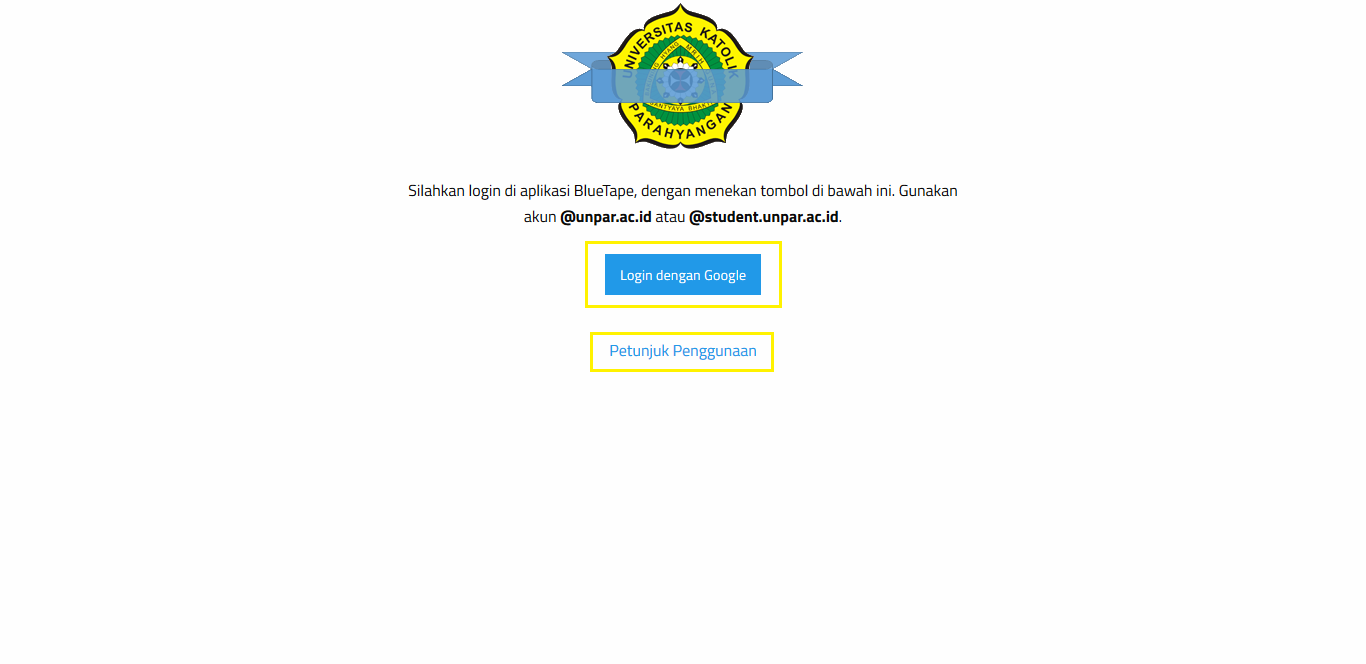
\includegraphics[scale=0.4, frame]{kriteria-sukses-1-4-3-contrast-minimum-1}  
        \caption[Pelanggaran Kriteria Sukses 1.4.3 pada Halaman \textit{Login}]{Pelanggaran Kriteria Sukses 1.4.3 pada Halaman \textit{Login}}
        \label{fig:1.4.3_contrast_minimum_1}  
    \end{figure} 
    
    \item Halaman cetak transkrip: 
    \begin{itemize}
        \item Teks "Kirim Permohonan" memiliki rasio kontras 3.09:1 terhadap warna latar belakangnya.
        \item Teks "Tercetak" di kolom status pada tabel memiliki rasio kontras 1.79:1 terhadap warna latar belakangnya.
        \item Teks "Ditolak" di kolom status pada tabel "Histori Permohonan" memiliki rasio kontras 3.44:1 terhadap warna latar belakangnya.
        \item Teks "Tunggu" di kolom status pada tabel "Histori Permohonan" memiliki rasio kontras 4.44:1 terhadap warna latar belakangnya.
    \end{itemize}   
    Tampilan pada halaman web dapat dilihat pada Gambar \ref{fig:1.4.3_contrast_minimum_2}. Tautan untuk halaman yang bermasalah dapat dilihat di \url{https://bluetape.azurewebsites.net/TranskripRequest}.
    \begin{figure}[H]
        \centering  
        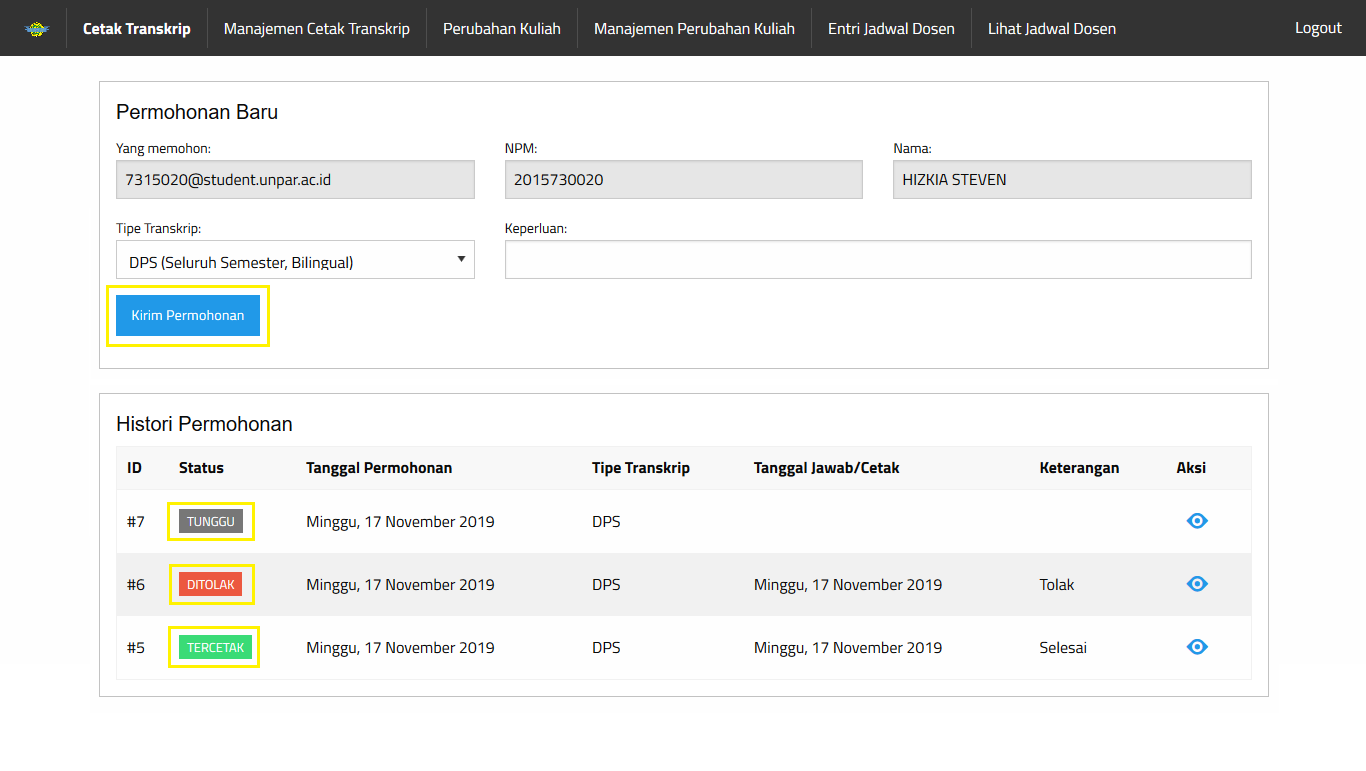
\includegraphics[scale=0.4, frame]{kriteria-sukses-1-4-3-contrast-minimum-2}  
        \caption[Pelanggaran Kriteria Sukses 1.4.3 pada Halaman Cetak Transkrip]{Pelanggaran Kriteria Sukses 1.4.3 pada Halaman Cetak Transkrip}
        \label{fig:1.4.3_contrast_minimum_2}  
    \end{figure} 
    
    \item Halaman manajemen cetak transkrip: 
    \begin{itemize}
        \item Teks "Cari" memiliki rasio kontras 3.09:1 terhadap warna latar belakangnya.
        \item Teks "Tercetak" di kolom status pada tabel memiliki rasio kontras 1.79:1 terhadap warna latar belakangnya.
        \item Teks "Menunggu" di kolom status pada tabel memiliki rasio kontras 1.84:1 terhadap warna latar belakangnya.
        \item Teks "Ditolak" di kolom status pada tabel memiliki rasio kontras 3.44:1 terhadap warna latar belakangnya.
        \item Teks "Hapus" pada bagian hapus permohonan memiliki rasio kontras 3.47:1 terhadap warna latar belakangnya.
    \end{itemize}
    Tampilan pada halaman web dapat dilihat pada Gambar \ref{fig:1.4.3_contrast_minimum_3_1} dan \ref{fig:1.4.3_contrast_minimum_3_2}. Tautan untuk halaman yang bermasalah dapat dilihat di \url{https://bluetape.azurewebsites.net/TranskripManage}.
    \begin{figure}[H]
        \centering  
        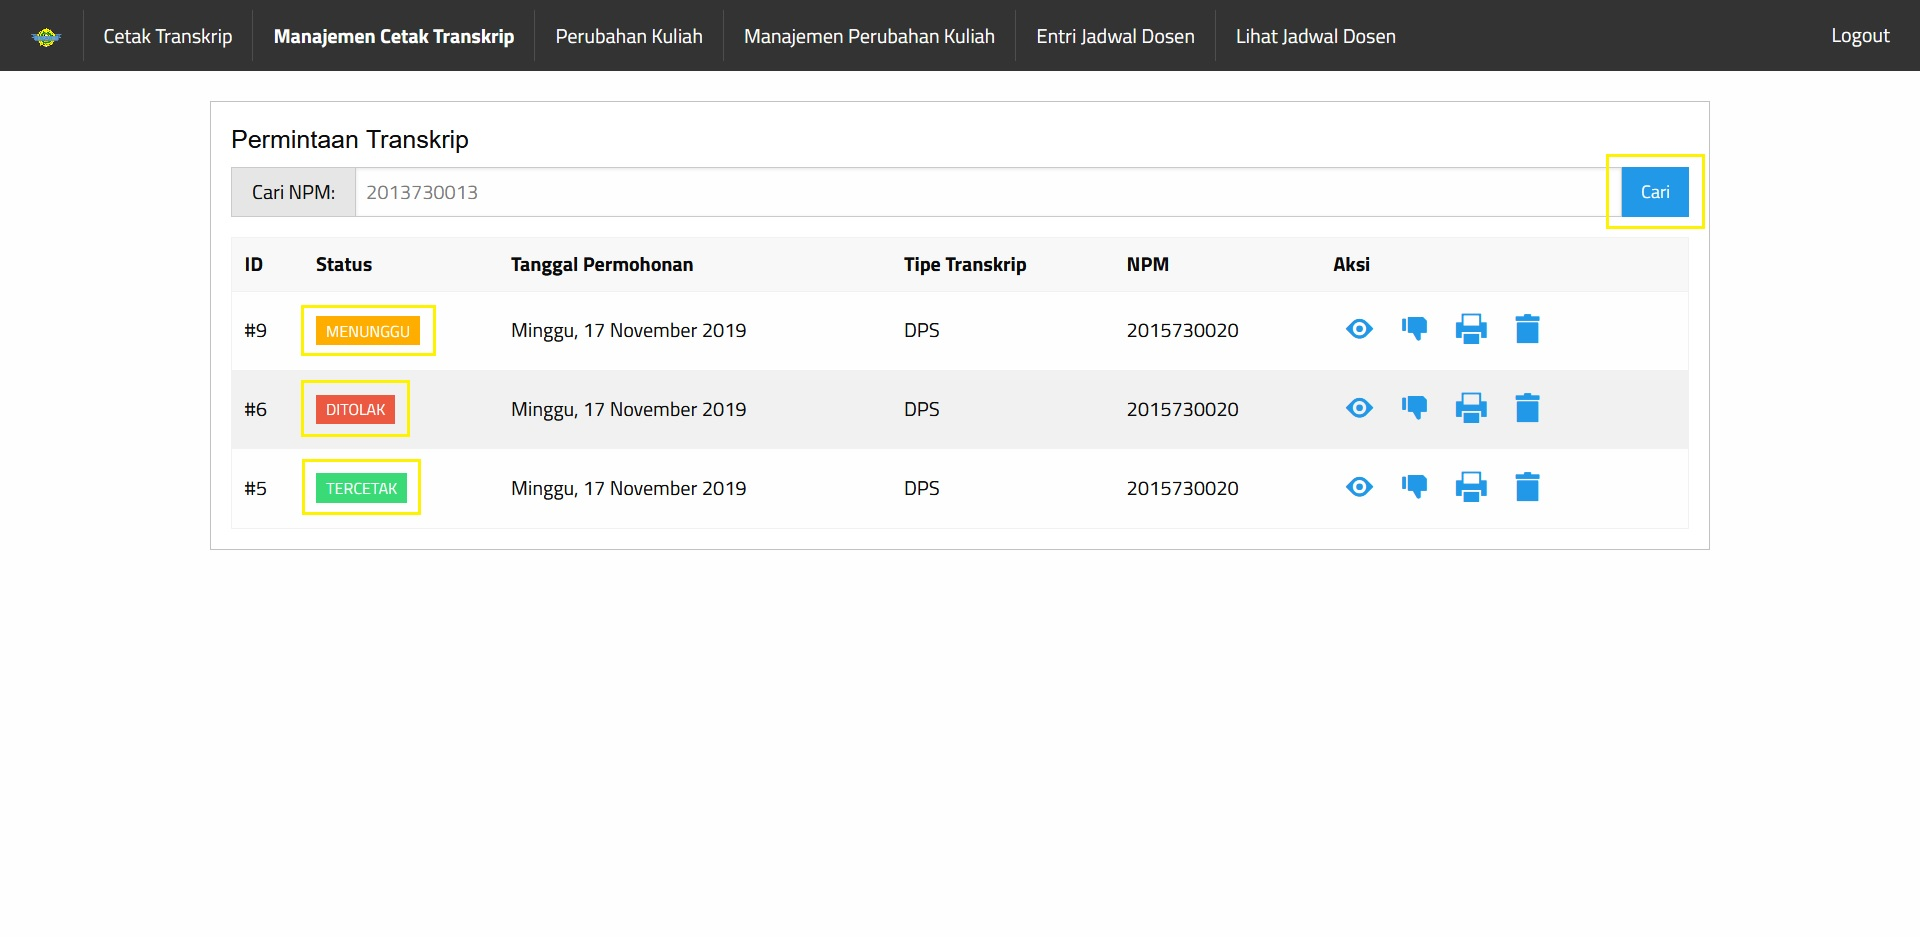
\includegraphics[scale=0.4, frame]{kriteria-sukses-1-4-3-contrast-minimum-3-1}  
        \caption[Pelanggaran Kriteria Sukses 1.4.3 pada Halaman Manajemen Cetak Transkrip]{Pelanggaran Kriteria Sukses 1.4.3 pada Halaman Manajemen Cetak Transkrip}
        \label{fig:1.4.3_contrast_minimum_3_1}
    \end{figure} 
    
    \begin{figure}[H]
        \centering  
        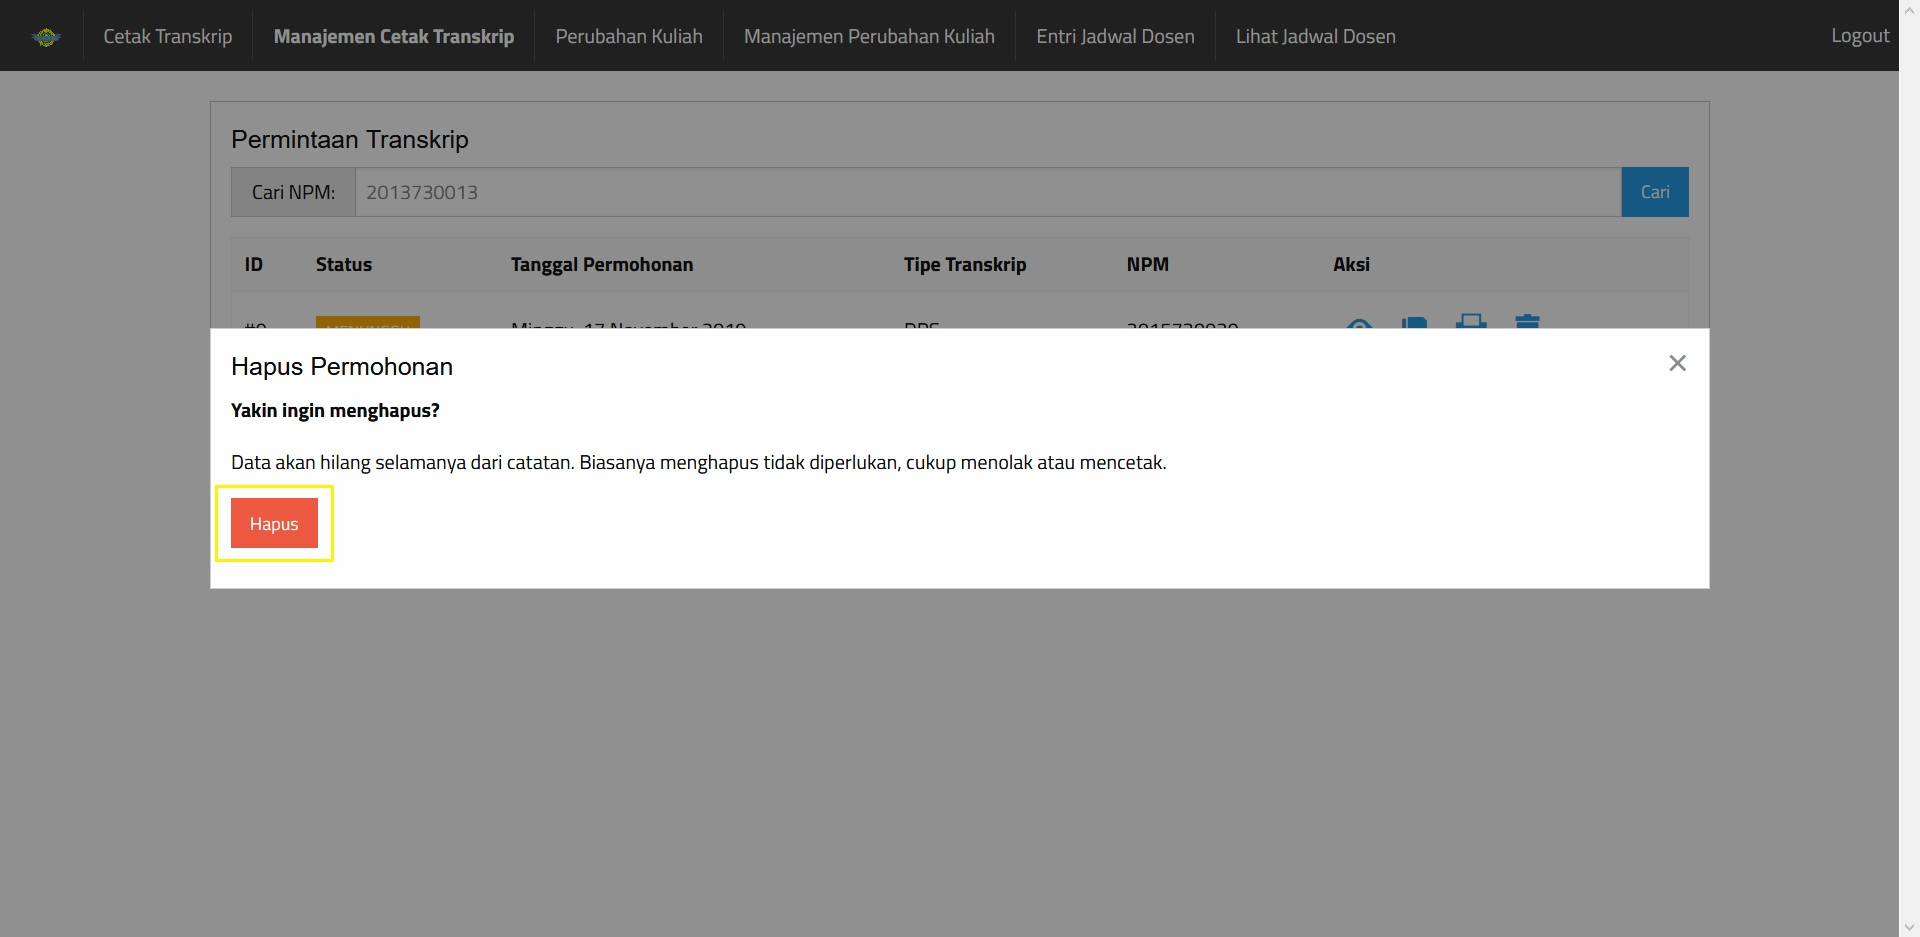
\includegraphics[scale=0.4, frame]{kriteria-sukses-1-4-3-contrast-minimum-3-2}  
        \caption[Pelanggaran Kriteria Sukses 1.4.3 pada Kotak Dialog di Halaman Manajemen Cetak Transkrip]{Pelanggaran Kriteria Sukses 1.4.3 pada Kotak Dialog di Halaman Manajemen Cetak Transkrip}
        \label{fig:1.4.3_contrast_minimum_3_2}
    \end{figure} 

    \item Halaman perubahan kuliah: 
    \begin{itemize}
        \item Teks "Kirim Permohonan" memiliki rasio kontras 3.09:1 terhadap warna latar belakangnya.
        \item Teks "Tambah Pertemuan Ekstra" memiliki rasio kontras 4.47:1 terhadap warna latar belakangnya.
        \item Teks "Hapus" memiliki rasio kontras 4.47:1 terhadap warna latar belakangnya.
        \item Teks "Tunggu" di kolom status pada tabel "Histori Permohonan" memiliki rasio kontras 4.44:1 terhadap warna latar belakangnya.
        \item Teks "Ditolak" di kolom status pada tabel "Histori Permohonan" memiliki rasio kontras 3.44:1 terhadap warna latar belakangnya.
        \item Teks "Terkonfirmasi" di kolom status pada tabel "Histori Permohonan" memiliki rasio kontras 1.79:1 terhadap warna latar belakangnya.
    \end{itemize}
    Tampilan pada halaman web dapat dilihat pada Gambar \ref{fig:1.4.3_contrast_minimum_4}. Tautan untuk halaman yang bermasalah dapat dilihat di \url{https://bluetape.azurewebsites.net/PerubahanKuliahRequest}.
    \begin{figure}[H]
        \centering  
        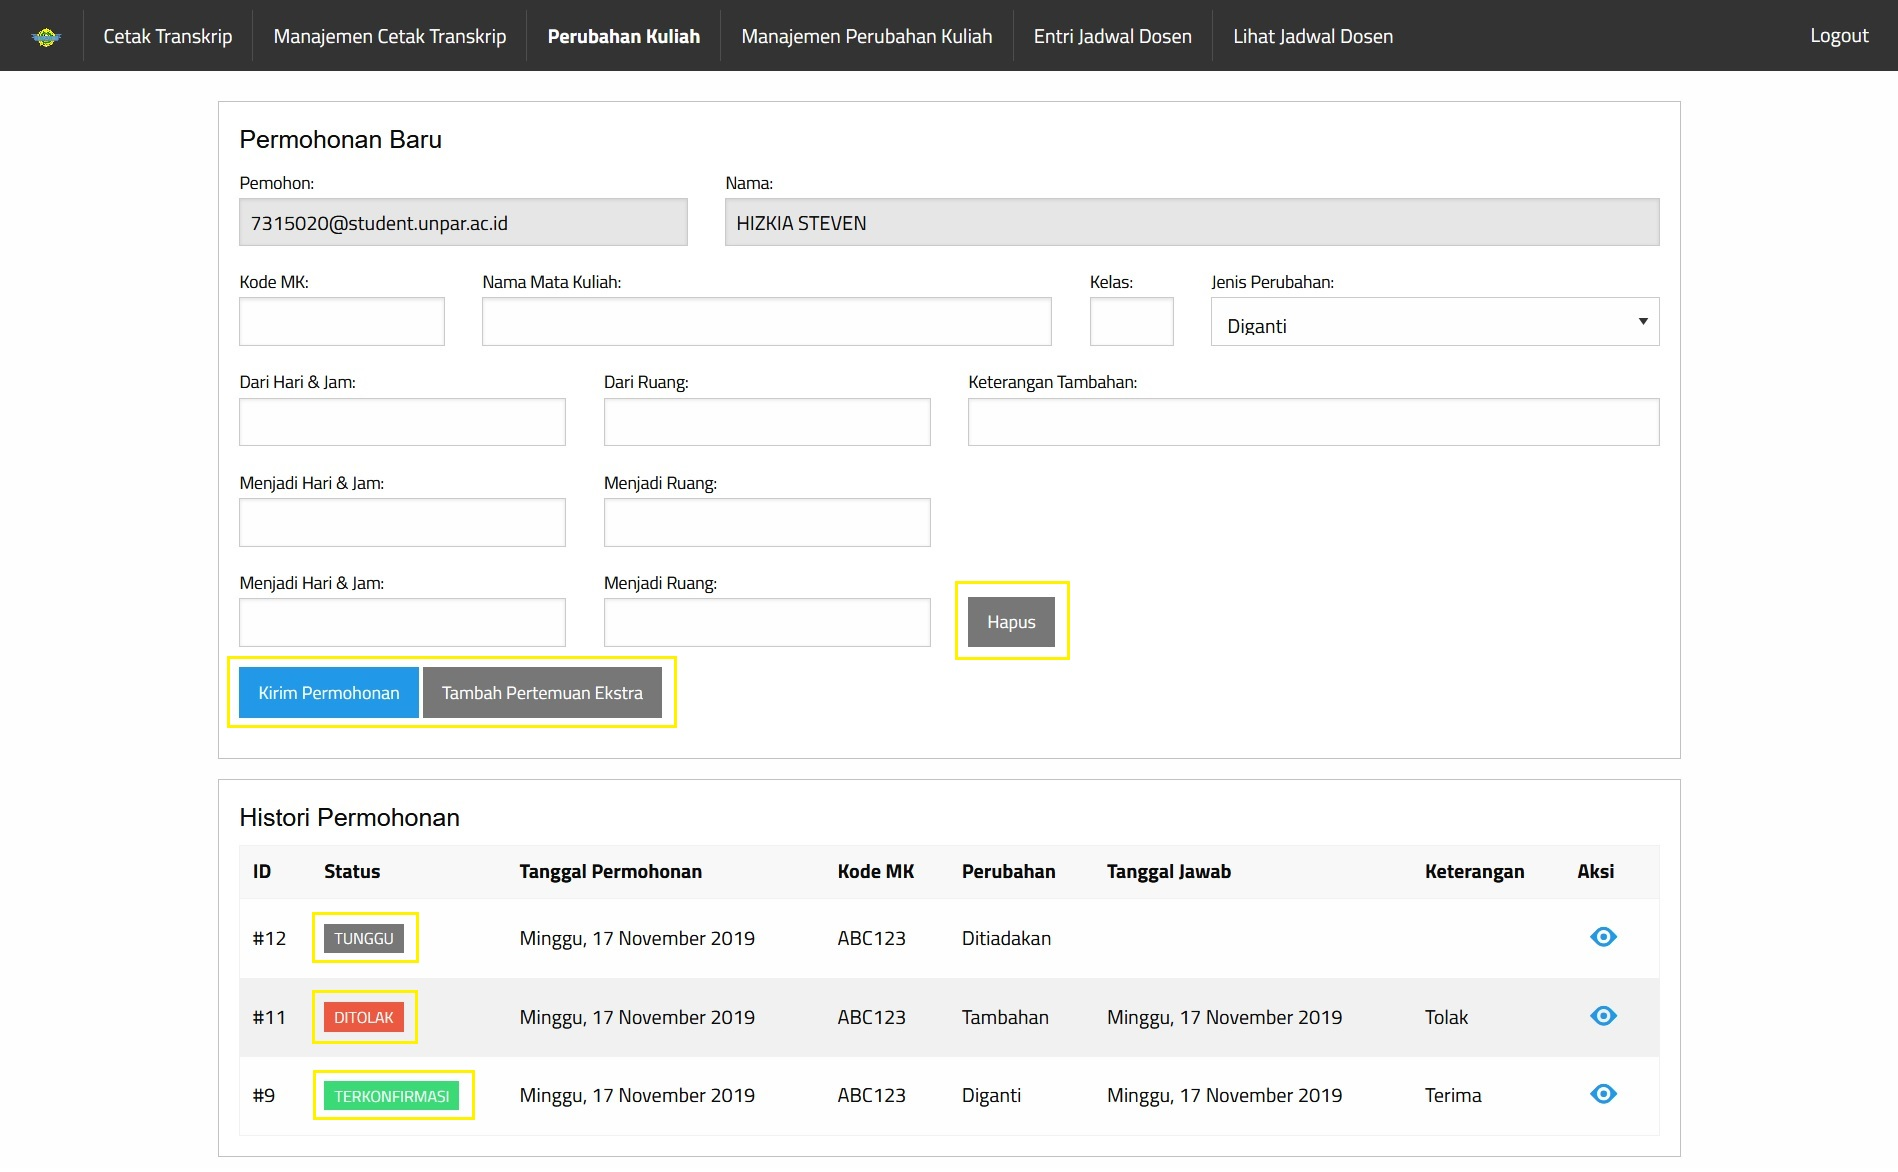
\includegraphics[scale=0.4, frame]{kriteria-sukses-1-4-3-contrast-minimum-4}  
        \caption[Pelanggaran Kriteria Sukses 1.4.3 pada Halaman Perubahan Kuliah]{Pelanggaran Kriteria Sukses 1.4.3 pada Halaman Perubahan Kuliah}
        \label{fig:1.4.3_contrast_minimum_4}  
    \end{figure} 
    
    \item Halaman manajemen perubahan kuliah: 
    \begin{itemize}
        \item Teks "Terkonfirmasi" di kolom status pada tabel memiliki rasio kontras 1.79:1 terhadap warna latar belakangnya.
        \item Teks "Menunggu" di kolom status pada tabel memiliki rasio kontras 1.84:1 terhadap warna latar belakangnya.
        \item Teks "Ditolak" di kolom status pada tabel memiliki rasio kontras 3.44:1 terhadap warna latar belakangnya.
        \item Teks "Hapus" pada bagian hapus permohonan memiliki rasio kontras 3.47:1 terhadap warna latar belakangnya.
    \end{itemize}
    Tampilan pada halaman web dapat dilihat pada Gambar \ref{fig:1.4.3_contrast_minimum_5_1} dan \ref{fig:1.4.3_contrast_minimum_5_2}. Tautan untuk halaman yang bermasalah dapat dilihat di \url{https://bluetape.azurewebsites.net/PerubahanKuliahManage}.
    \begin{figure}[H]
        \centering  
        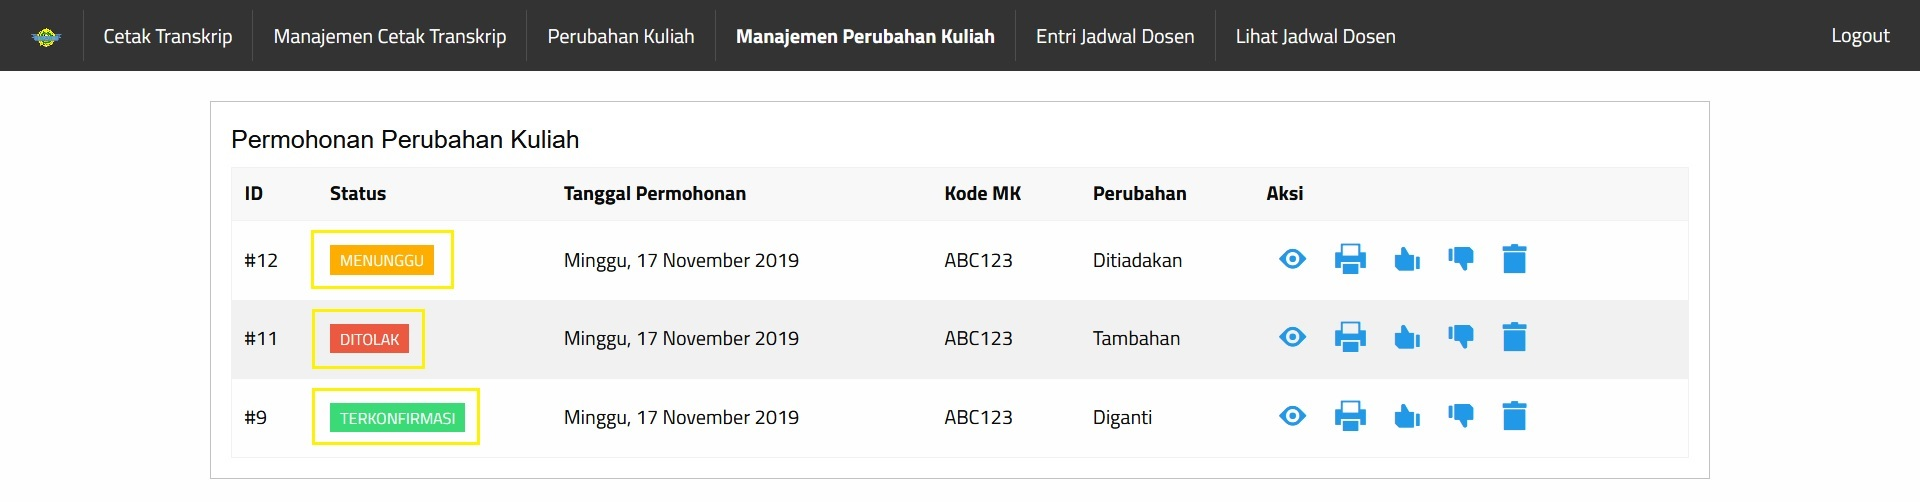
\includegraphics[scale=0.4, frame]{kriteria-sukses-1-4-3-contrast-minimum-5-1}  
        \caption[Pelanggaran Kriteria Sukses 1.4.3 pada Halaman Manajemen Perubahan Kuliah]{Pelanggaran Kriteria Sukses 1.4.3 pada Halaman Manajemen Perubahan Kuliah}
        \label{fig:1.4.3_contrast_minimum_5_1}
    \end{figure} 
    
    \begin{figure}[H]
        \centering  
        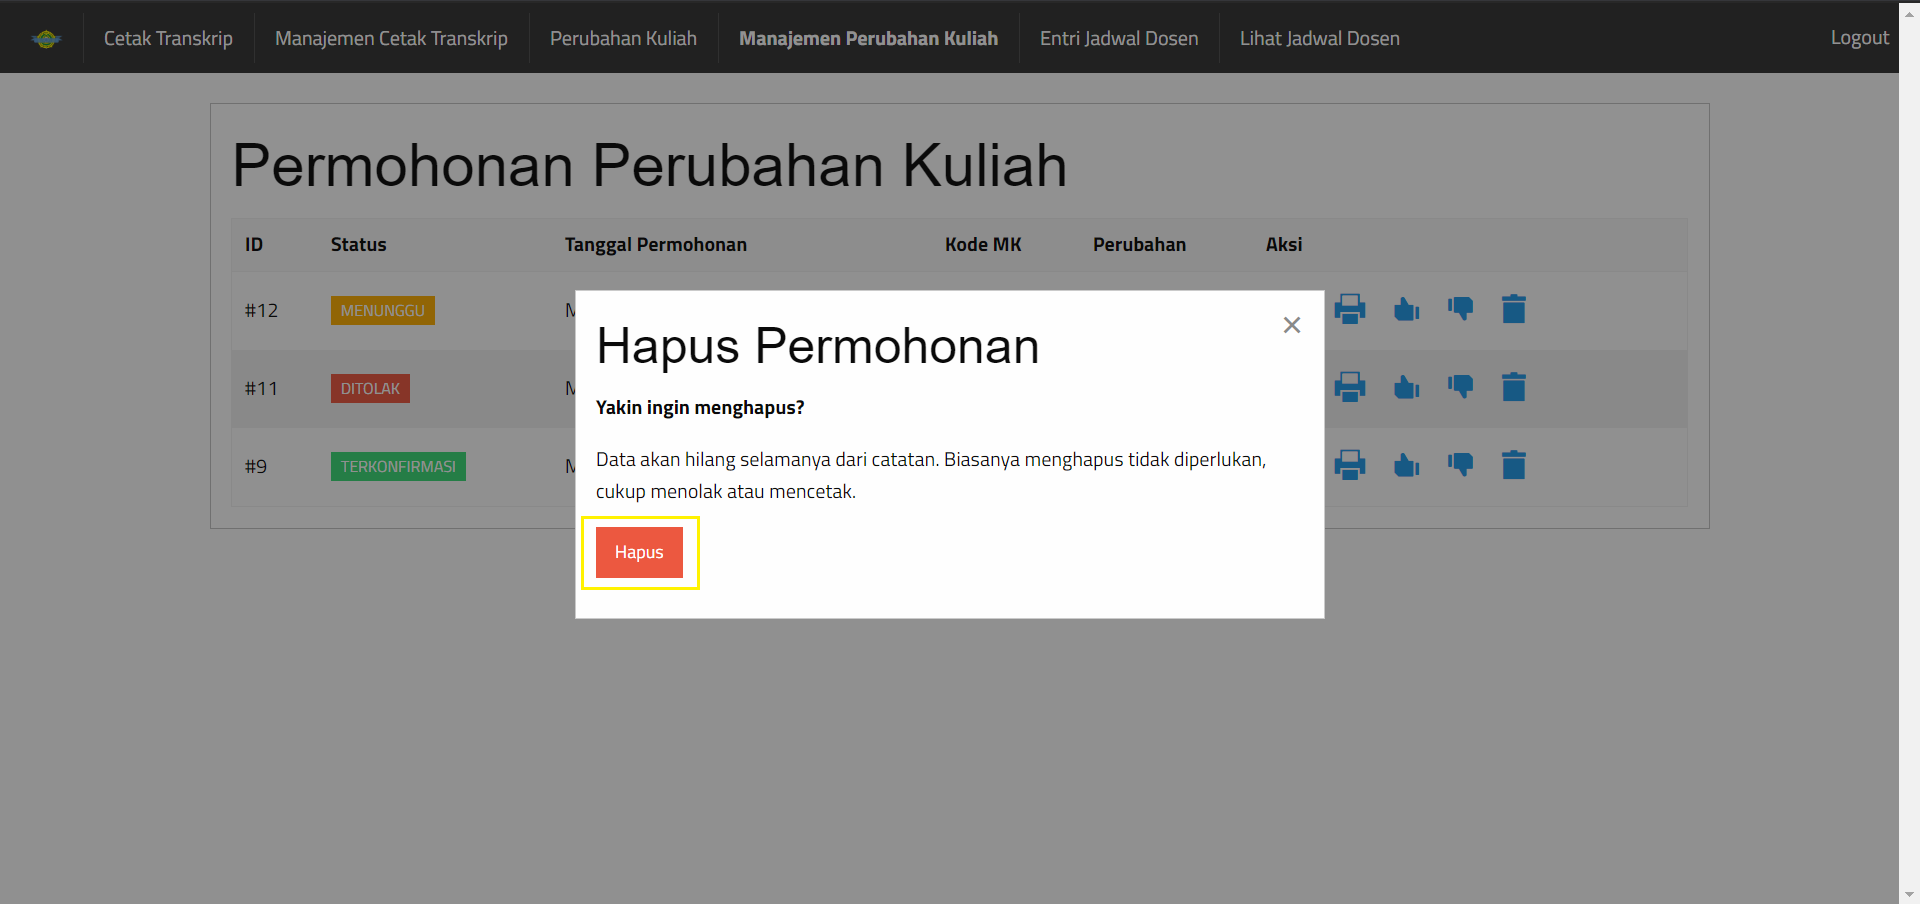
\includegraphics[scale=0.4, frame]{kriteria-sukses-1-4-3-contrast-minimum-5-2}  
        \caption[Pelanggaran Kriteria Sukses 1.4.3 pada Kotak Dialog di Halaman Manajemen Perubahan Kuliah]{Pelanggaran Kriteria Sukses 1.4.3 pada Kotak Dialog di Halaman Manajemen Perubahan Kuliah}
        \label{fig:1.4.3_contrast_minimum_5_2}
    \end{figure} 

    \item Halaman entri jadwal dosen: 
    \begin{itemize}
        \item Teks "Tambah" memiliki rasio kontras 3.09:1 terhadap warna latar belakangnya.
        \item Teks "Delete All" memiliki rasio kontras 3.47:1 terhadap warna latar belakangnya.
        \item Teks "Ekspor ke XLS" memiliki rasio kontras 3.09:1 terhadap warna latar belakangnya.
        \item Teks "Save" pada bagian "Edit Jadwal" memiliki rasio kontras 3.09:1 terhadap warna latar belakangnya.
        \item Teks "Delete" memiliki rasio kontras 3.47:1 terhadap warna latar belakangnya.
    \end{itemize}
    Tampilan pada halaman web dapat dilihat pada Gambar \ref{fig:1.4.3_contrast_minimum_6_1} dan \ref{fig:1.4.3_contrast_minimum_6_2}. Tautan untuk halaman yang bermasalah dapat dilihat di \url{https://bluetape.azurewebsites.net/EntriJadwalDosen}.	
    \begin{figure}[H]
        \centering  
        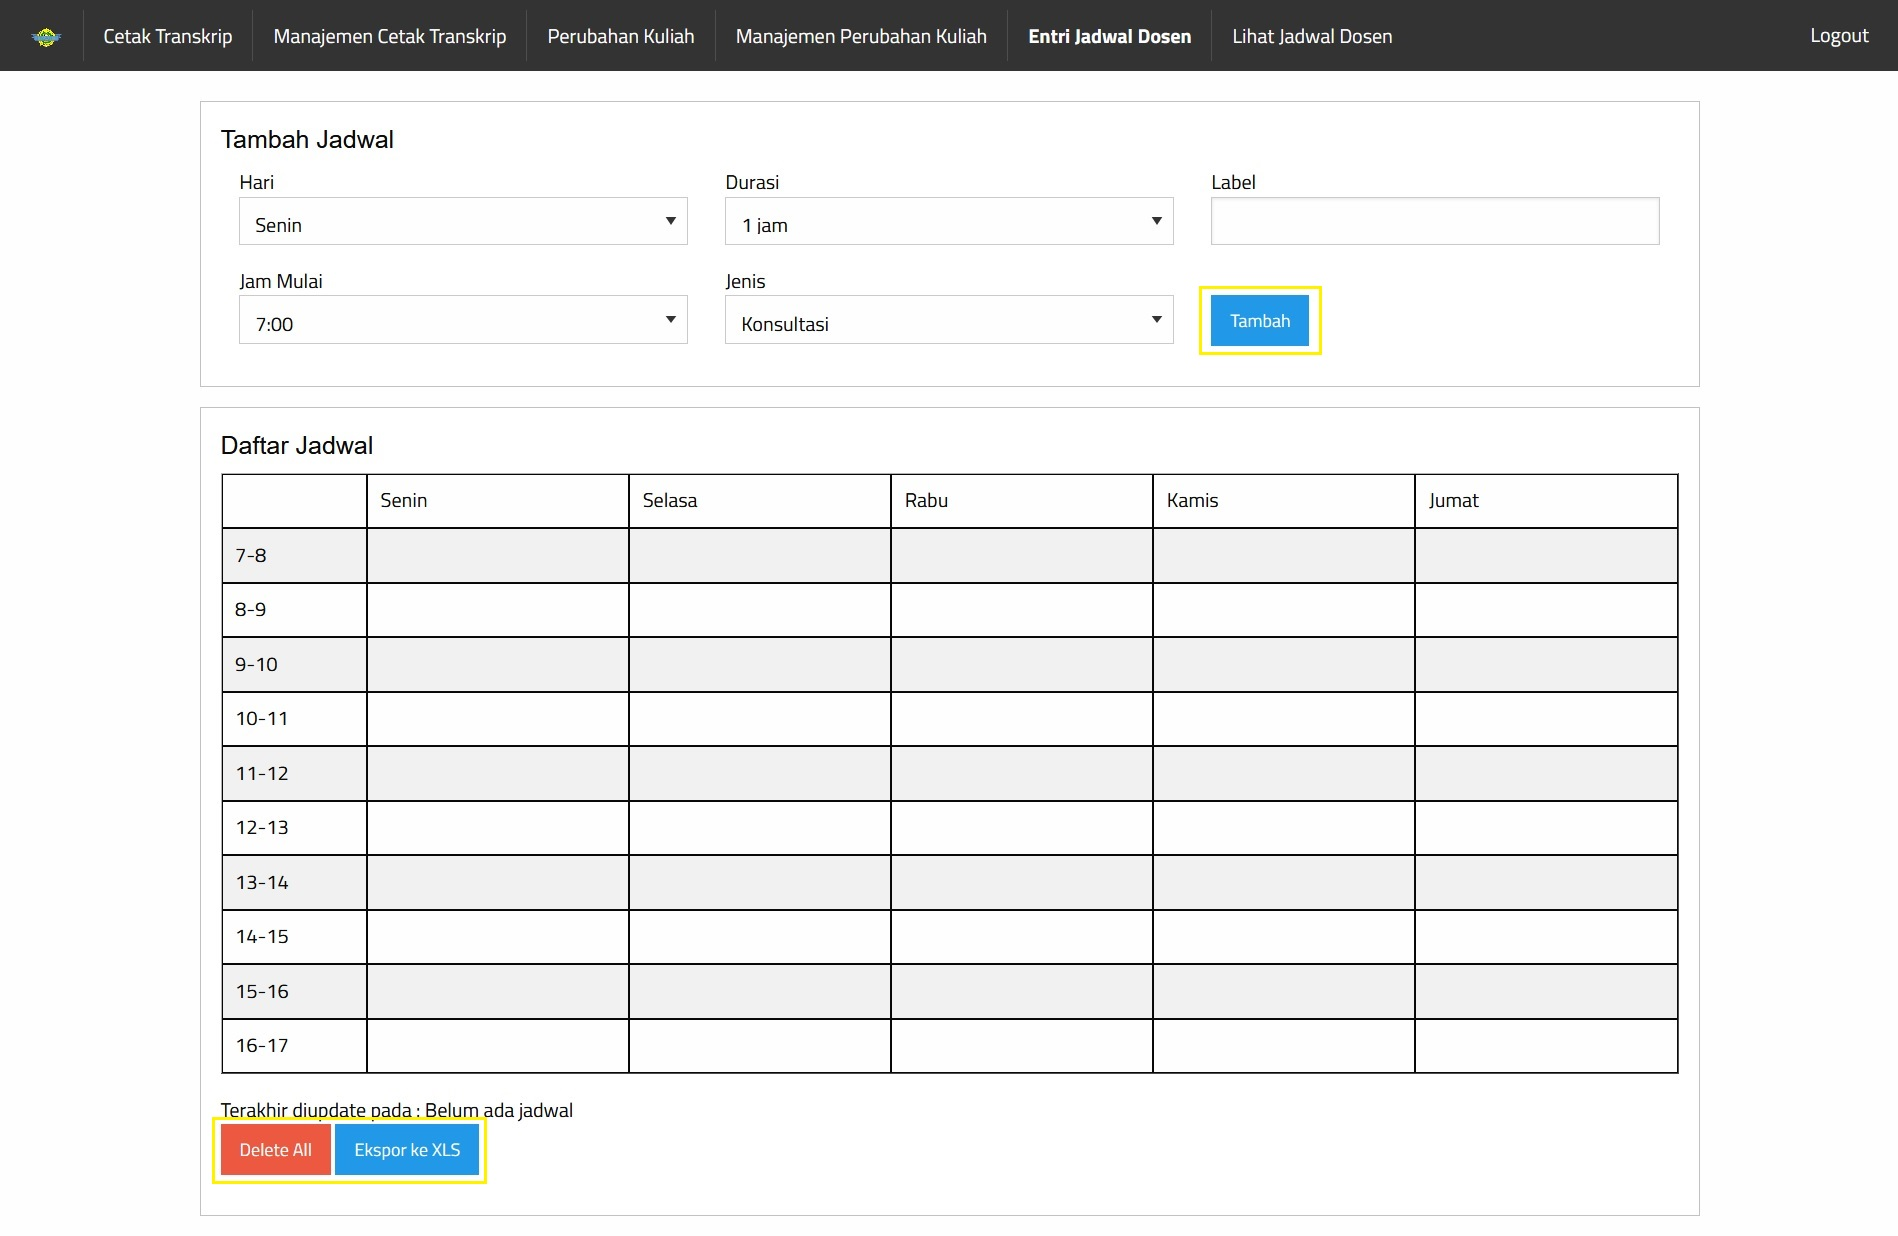
\includegraphics[scale=0.4, frame]{kriteria-sukses-1-4-3-contrast-minimum-6-1}  
        \caption[Pelanggaran Kriteria Sukses 1.4.3 pada Halaman Entri Jadwal Dosen]{Pelanggaran Kriteria Sukses 1.4.3 pada Halaman Entri Jadwal Dosen}
        \label{fig:1.4.3_contrast_minimum_6_1}  
    \end{figure} 
    
    \begin{figure}[H]
        \centering  
        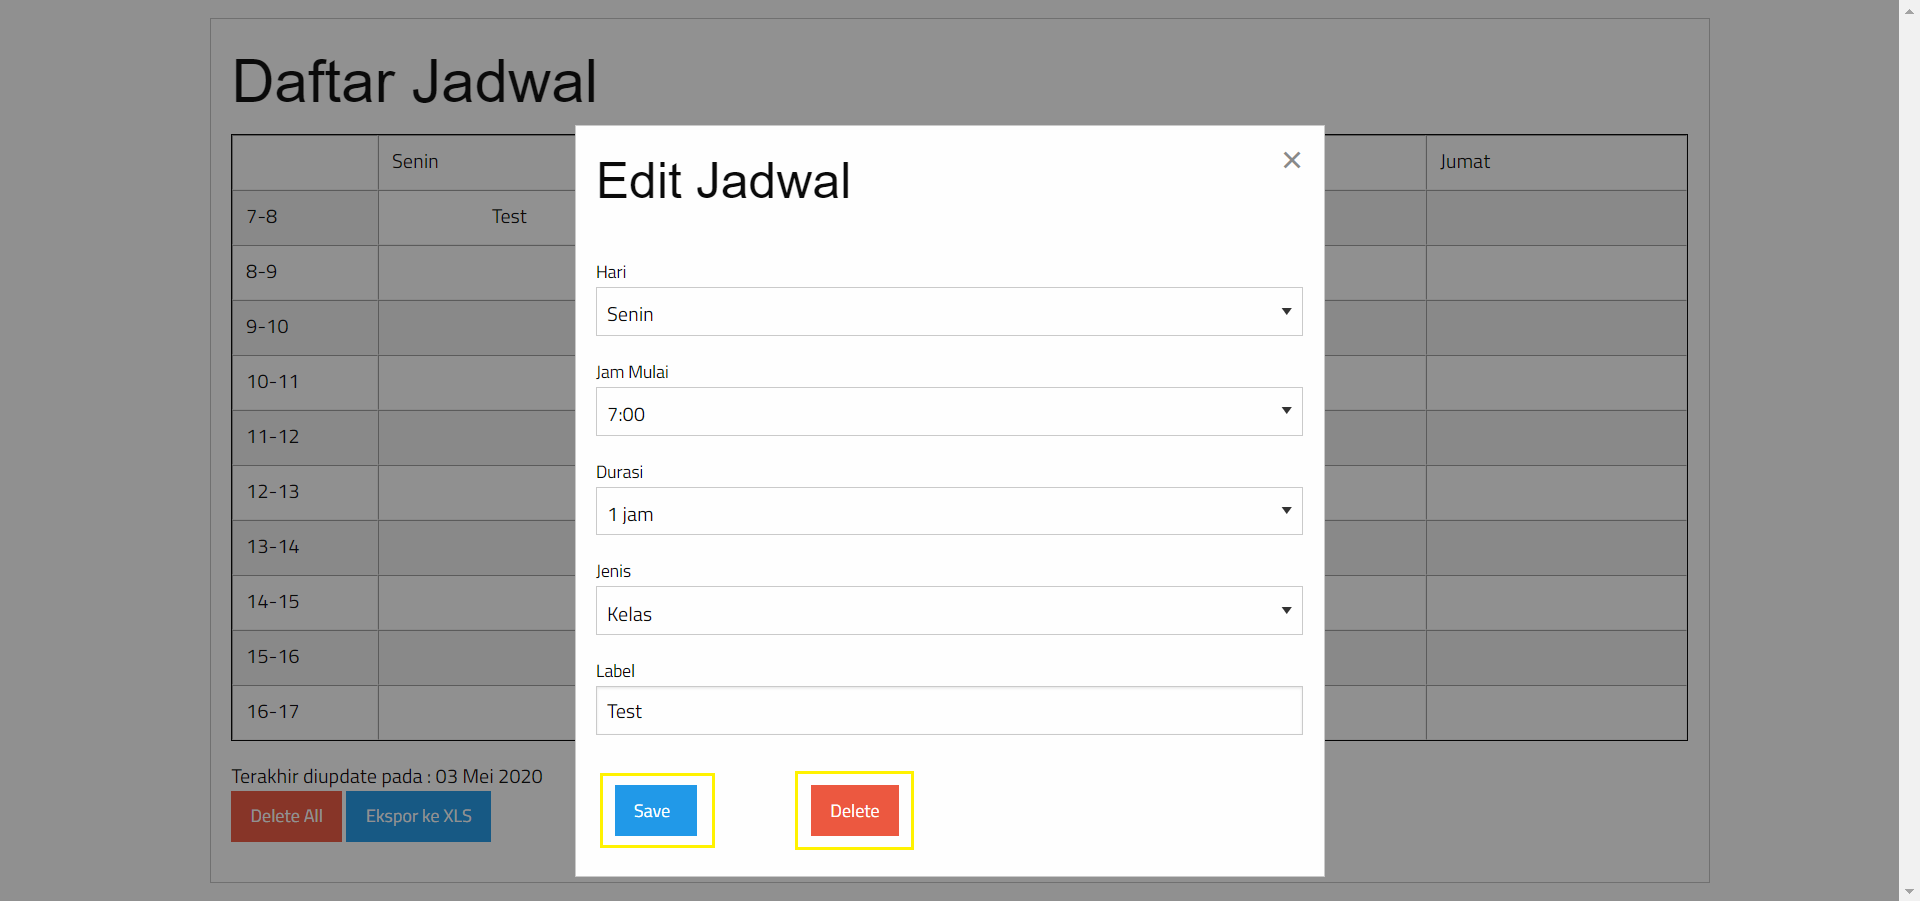
\includegraphics[scale=0.4, frame]{kriteria-sukses-1-4-3-contrast-minimum-6-2}  
        \caption[Pelanggaran Kriteria Sukses 1.4.3 pada Kotak Dialog di Halaman Entri Jadwal Dosen]{Pelanggaran Kriteria Sukses 1.4.3 pada Kotak Dialog di Halaman Entri Jadwal Dosen}
        \label{fig:1.4.3_contrast_minimum_6_2}  
    \end{figure} 

    \item Halaman lihat jadwal dosen: 
    \begin{itemize}
        \item Teks nama dosen di atas tabel yang sedang dipilih pengguna memiliki rasio kontras 2.47:1 terhadap warna latar belakangnya.
        \item Teks nama dosen di atas tabel yang sedang tidak dipilih pengguna memiliki rasio kontras 3.06:1 terhadap warna latar belakangnya.
        \item Teks "Ekspor ke XLS" memiliki rasio kontras 3.09:1 terhadap warna latar belakangnya.
    \end{itemize}
    Tampilan pada halaman web dapat dilihat pada Gambar \ref{fig:1.4.3_contrast_minimum_7}. Tautan untuk halaman yang bermasalah dapat dilihat di \url{https://bluetape.azurewebsites.net/LihatJadwalDosen}.
    \begin{figure}[H]
        \centering  
        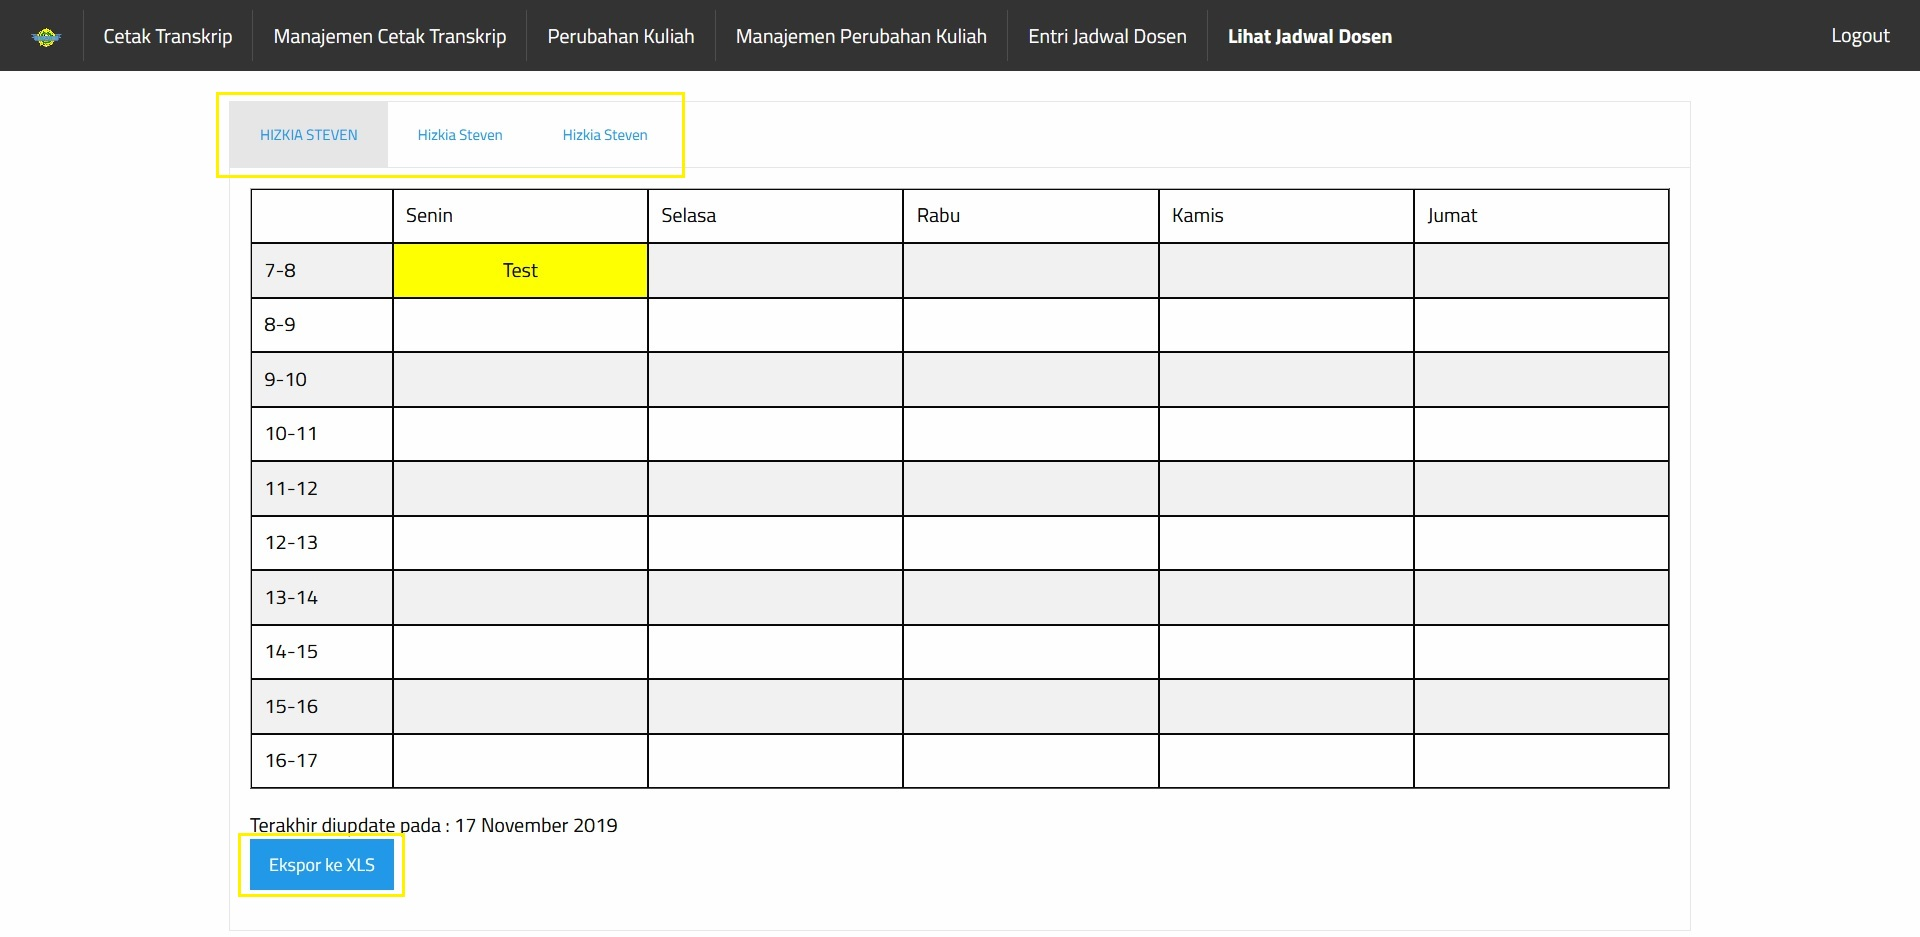
\includegraphics[scale=0.4, frame]{kriteria-sukses-1-4-3-contrast-minimum-7}  
        \caption[Pelanggaran Kriteria Sukses 1.4.3 pada Halaman Lihat Jadwal Dosen]{Pelanggaran Kriteria Sukses 1.4.3 pada Halaman Lihat Jadwal Dosen}
        \label{fig:1.4.3_contrast_minimum_7}  
    \end{figure} 
\end{itemize}

\paragraph{Kriteria Sukses 1.4.4 \textit{Resize text}}
\label{par:kepatuhan_bluetape_kriteria_sukses_1.4.4}
(Sukses)\\

Kriteria ini sukses dipatuhi karena setiap halaman web BlueTape dapat tetap terbaca dan tidak kehilangan fungsionalitasnya ketika halaman diperbesar hingga 200 persen. 

\paragraph{Kriteria Sukses 1.4.5 \textit{Images of Text}}
\label{par:kepatuhan_bluetape_kriteria_sukses_1.4.5}
(Sukses)\\

Kriteria ini sukses dipatuhi karena pada halaman web BlueTape tidak terdapat gambar teks selain logo.

\paragraph{Kriteria Sukses 1.4.6 \textit{Contrast (Enhanced)}}
\label{par:kepatuhan_bluetape_kriteria_sukses_1.4.6}
(Tidak Sukses)\\

Kriteria ini tidak sukses dipatuhi karena pada halaman web BlueTape terdapat beberapa teks dengan rasio kontras kurang dari 7:1 untuk teks yang berukuran kurang dari 24 piksel dan tidak \textit{bold}. Nilai rasio kontras didapatkan dengan menggunakan bantuan \textit{extension} axe pada \textit{browser} Google Chrome, penguji bernavigasi ke seluruh halaman web BlueTape lalu menggunakan alat tersebut untuk mendeteksi bagian yang bermasalah. Bagian-bagian yang tidak memenuhi syarat untuk kriteria ini, antara lain:

\begin{itemize}
    \item Halaman \textit{login}: 
    \begin{itemize}
        \item Teks "\textit{Login} dengan Google" memiliki rasio kontras 3.09:1 terhadap warna latar belakangnya.
        \item Teks "Petunjuk Penggunaan" memiliki rasio kontras 3.06:1 terhadap warna latar belakangnya.
    \end{itemize}
    Tampilan pada halaman web dapat dilihat pada Gambar \ref{fig:1.4.6_contrast_enchanced_1}. Tautan untuk halaman yang bermasalah dapat dilihat di \url{https://bluetape.azurewebsites.net}.
    \begin{figure}[H]
        \centering  
        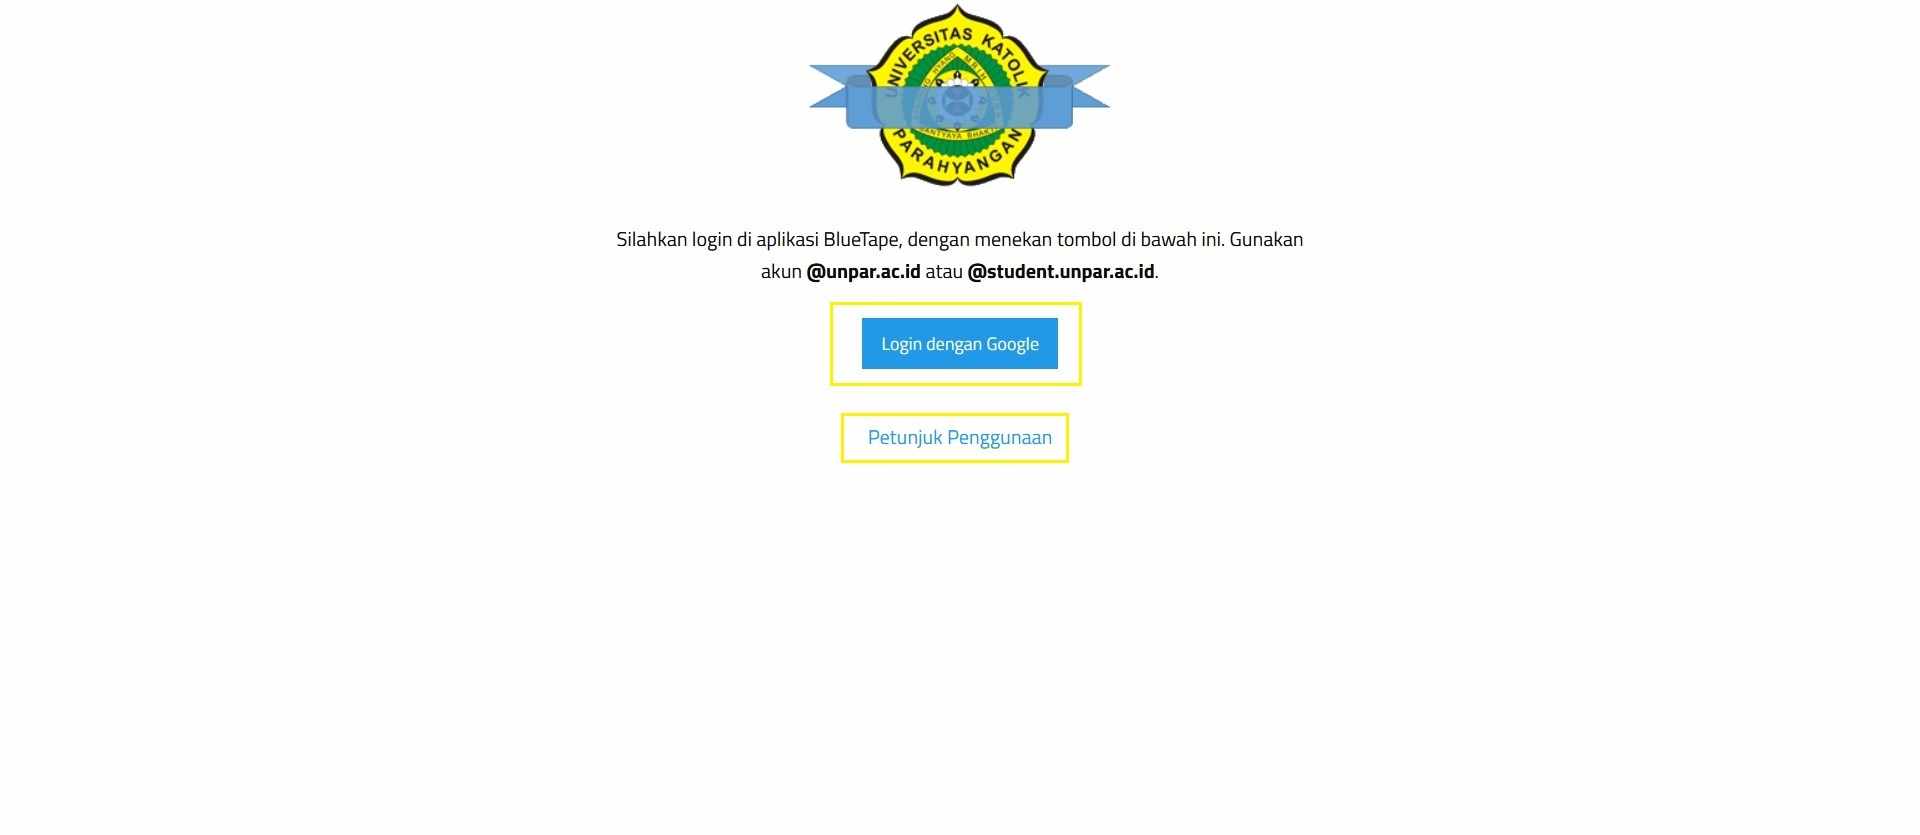
\includegraphics[scale=0.4, frame]{kriteria-sukses-1-4-6-contrast-enchanced-1}  
        \caption[Pelanggaran Kriteria Sukses 1.4.6 pada Halaman \textit{Login}]{Pelanggaran Kriteria Sukses 1.4.6 pada Halaman \textit{Login}}
        \label{fig:1.4.6_contrast_enchanced_1}  
    \end{figure} 

    \item Halaman cetak transkrip: 
    \begin{itemize}
        \item Teks "Kirim Permohonan" memiliki rasio kontras 3.09:1 terhadap warna latar belakangnya.
        \item Teks "Tercetak" di kolom status pada tabel memiliki rasio kontras 1.79:1 terhadap warna latar belakangnya.
        \item Teks "Ditolak" di kolom status pada tabel "Histori Permohonan" memiliki rasio kontras 3.44:1 terhadap warna latar belakangnya.
        \item Teks "Tunggu" di kolom status pada tabel "Histori Permohonan" memiliki rasio kontras 4.44:1 terhadap warna latar belakangnya.
    \end{itemize}
    Tampilan pada halaman web dapat dilihat pada Gambar \ref{fig:1.4.6_contrast_enchanced_2}. Tautan untuk halaman yang bermasalah dapat dilihat di \url{https://bluetape.azurewebsites.net/TranskripRequest}.
    \begin{figure}[H]
        \centering  
        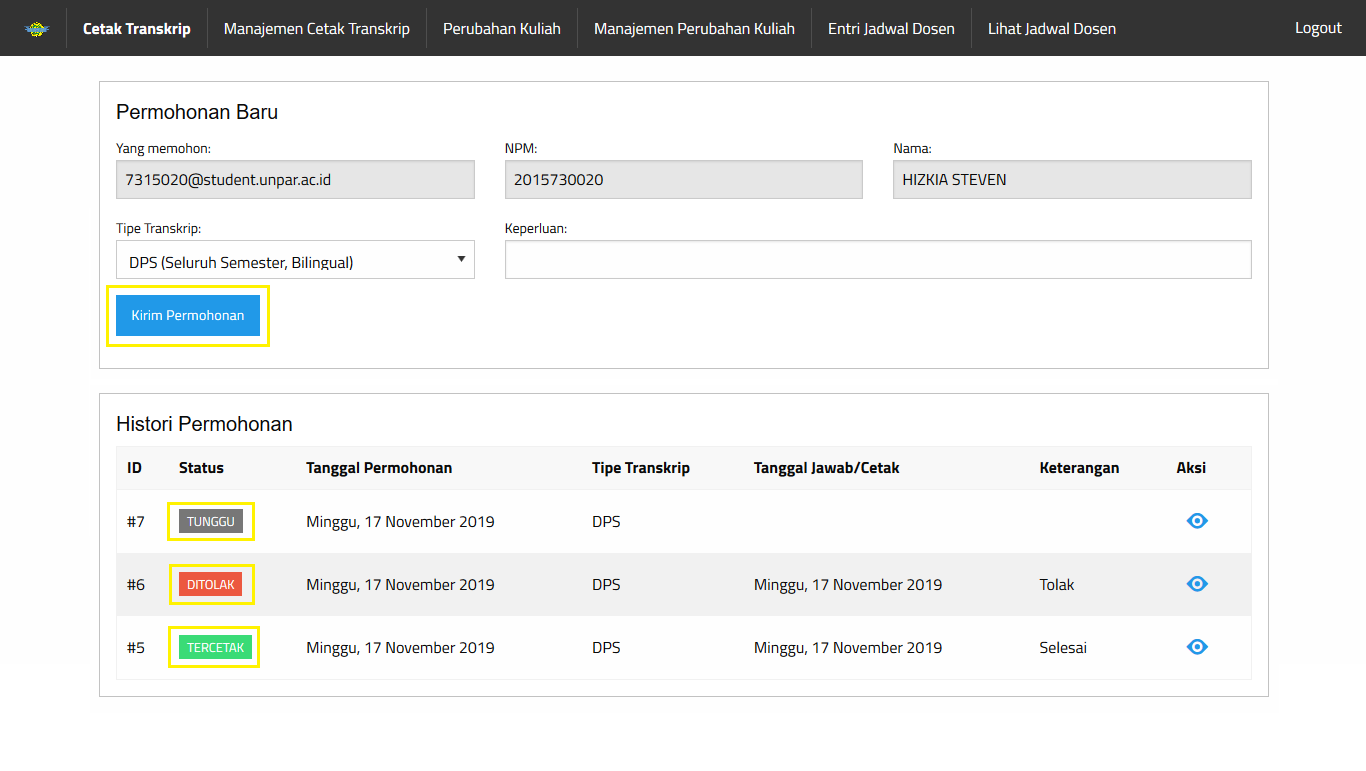
\includegraphics[scale=0.4, frame]{kriteria-sukses-1-4-6-contrast-enchanced-2}  
        \caption[Pelanggaran Kriteria Sukses 1.4.6 pada Halaman Cetak Transkrip]{Pelanggaran Kriteria Sukses 1.4.6 pada Halaman Cetak Transkrip}
        \label{fig:1.4.6_contrast_enchanced_2}  
    \end{figure} 
    
    \item Halaman manajemen cetak transkrip: 
    \begin{itemize}
        \item Teks "Cari" memiliki rasio kontras 3.09:1 terhadap warna latar belakangnya.
        \item Teks "Tercetak" di kolom status pada tabel memiliki rasio kontras 1.79:1 terhadap warna latar belakangnya.
        \item Teks "Menunggu" di kolom status pada tabel memiliki rasio kontras 1.84:1 terhadap warna latar belakangnya.
        \item Teks "Ditolak" di kolom status pada tabel memiliki rasio kontras 3.44:1 terhadap warna latar belakangnya.
        \item Teks "Hapus" pada bagian hapus permohonan memiliki rasio kontras 3.47:1 terhadap warna latar belakangnya.
    \end{itemize}
    Tampilan pada halaman web dapat dilihat pada Gambar \ref{fig:1.4.6_contrast_enchanced_3_1} dan \ref{fig:1.4.6_contrast_enchanced_3_2}. Tautan untuk halaman yang bermasalah dapat dilihat di \url{https://bluetape.azurewebsites.net/TranskripManage}.
    \begin{figure}[H]
        \centering  
        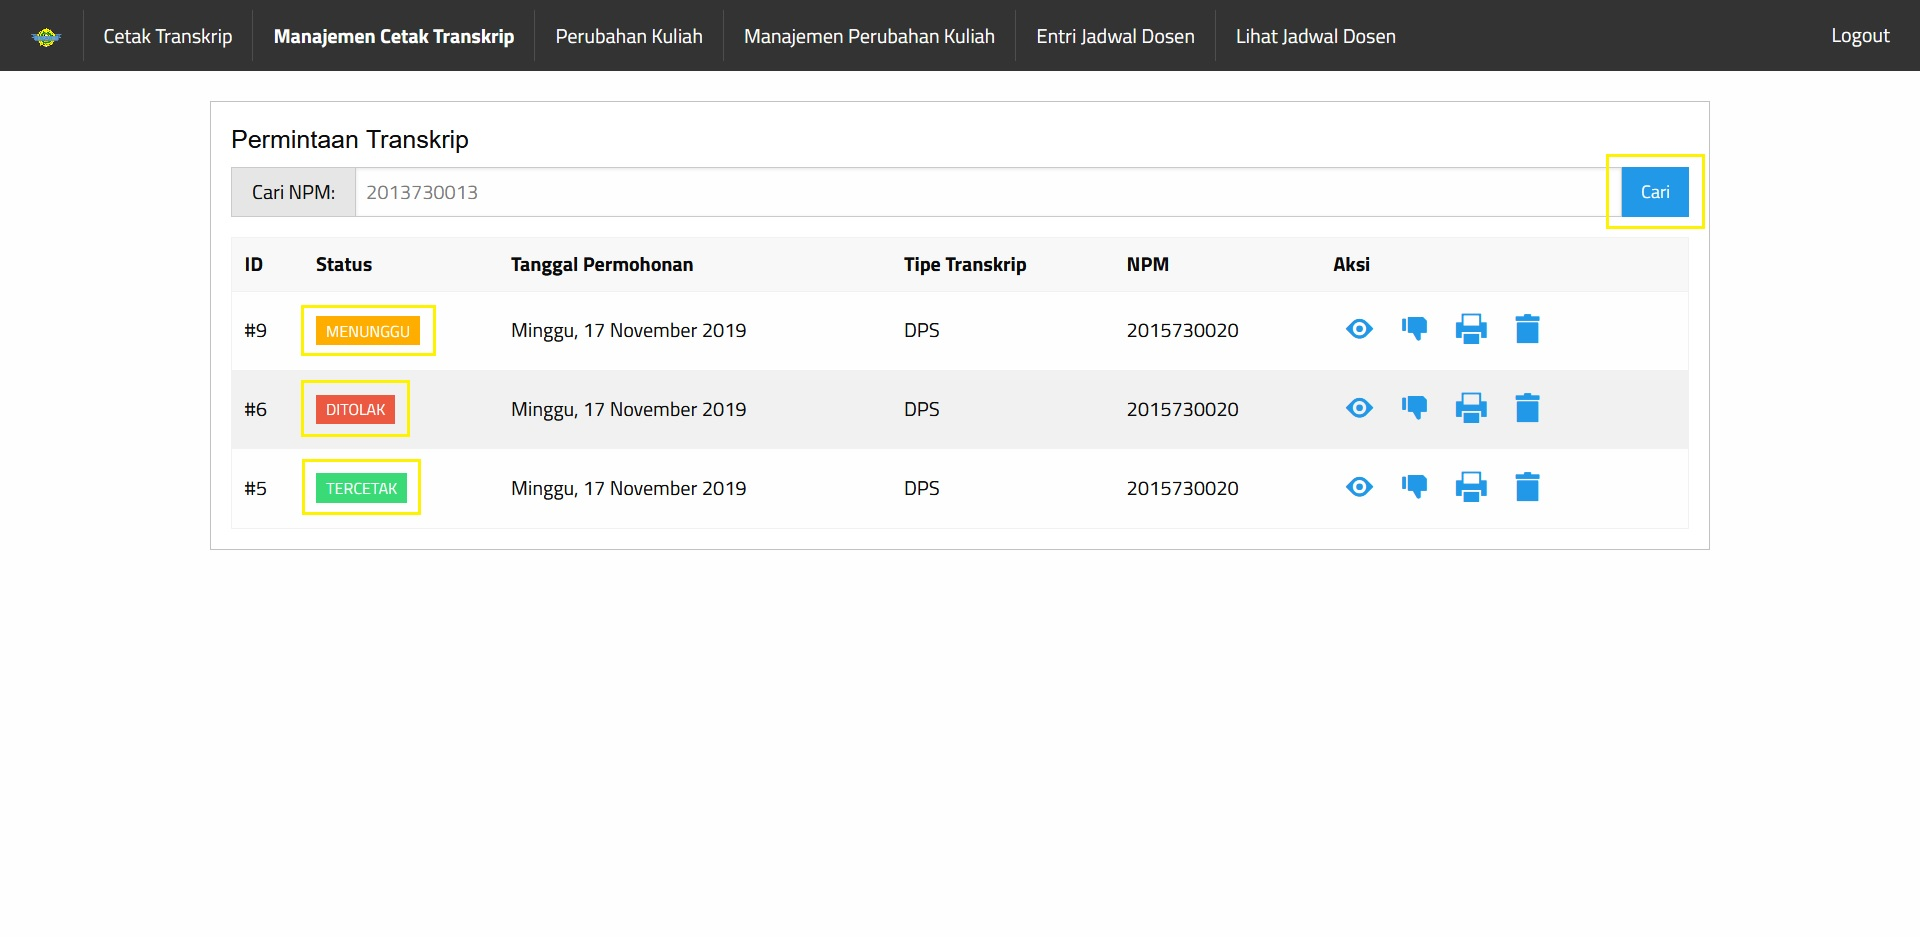
\includegraphics[scale=0.4, frame]{kriteria-sukses-1-4-6-contrast-enchanced-3-1}  
        \caption[Pelanggaran Kriteria Sukses 1.4.6 pada Halaman Manajemen Cetak Transkrip ]{Pelanggaran Kriteria Sukses 1.4.6 pada Halaman Manajemen Cetak Transkrip}
        \label{fig:1.4.6_contrast_enchanced_3_1}  
    \end{figure} 
    
    \begin{figure}[H]
        \centering  
        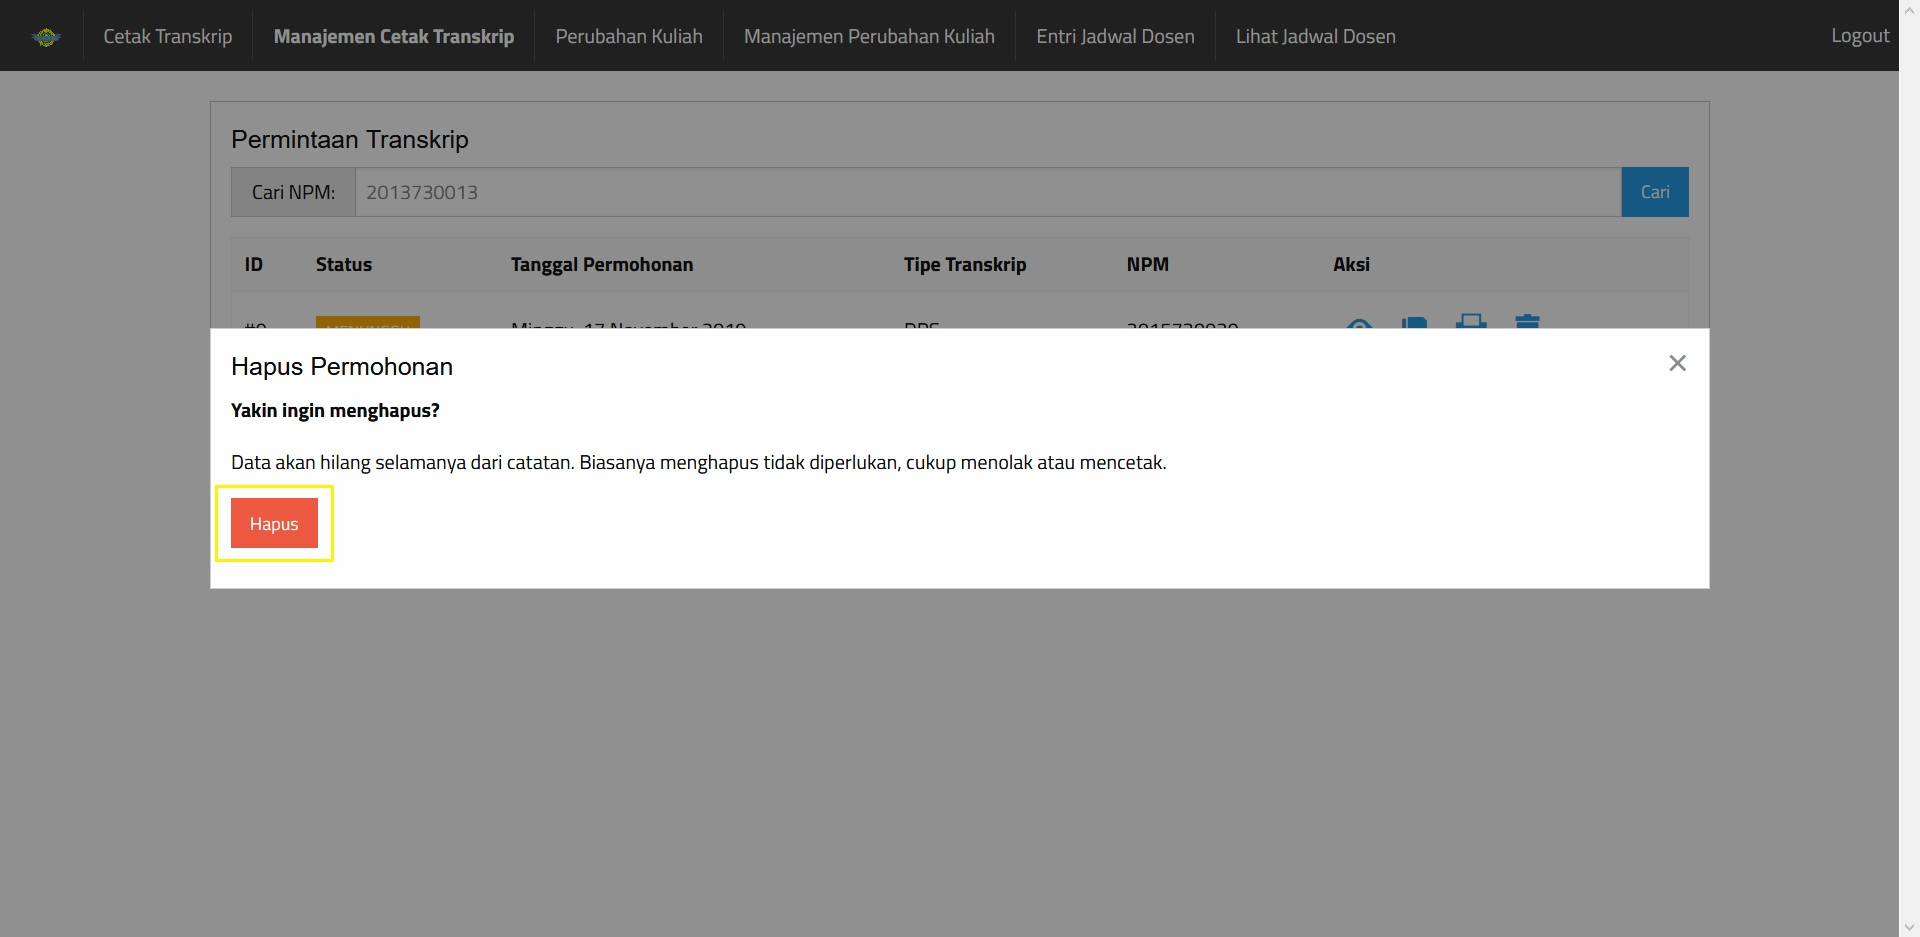
\includegraphics[scale=0.4, frame]{kriteria-sukses-1-4-6-contrast-enchanced-3-2}  
        \caption[Pelanggaran Kriteria Sukses 1.4.6 pada Kotak Dialog di Halaman Manajemen Cetak Transkrip]{Pelanggaran Kriteria Sukses 1.4.6 pada Kotak Dialog di Halaman Manajemen Cetak Transkrip}
        \label{fig:1.4.6_contrast_enchanced_3_2}  
    \end{figure} 

    \item Halaman perubahan kuliah: 
    \begin{itemize}
        \item Teks "Kirim Permohonan" memiliki rasio kontras 3.09:1 terhadap warna latar belakangnya.
        \item Teks "Tambah Pertemuan Ekstra" memiliki rasio kontras 4.47:1 terhadap warna latar belakangnya.
        \item Teks "Hapus" memiliki rasio kontras 4.47:1 terhadap warna latar belakangnya. 
        \item Teks "Tunggu" di kolom status pada tabel "Histori Permohonan" memiliki rasio kontras 4.44:1 terhadap warna latar belakangnya.
        \item Teks "Ditolak" di kolom status pada tabel "Histori Permohonan" memiliki rasio kontras 3.44:1 terhadap warna latar belakangnya.
        \item Teks "Terkonfirmasi" di kolom status pada tabel "Histori Permohonan" memiliki rasio kontras 1.79:1 terhadap warna latar belakangnya.
    \end{itemize}
    Tampilan pada halaman web dapat dilihat pada Gambar \ref{fig:1.4.6_contrast_enchanced_4}. Tautan untuk halaman yang bermasalah dapat dilihat di \url{https://bluetape.azurewebsites.net/PerubahanKuliahRequest}.
    \begin{figure}[H]
        \centering  
        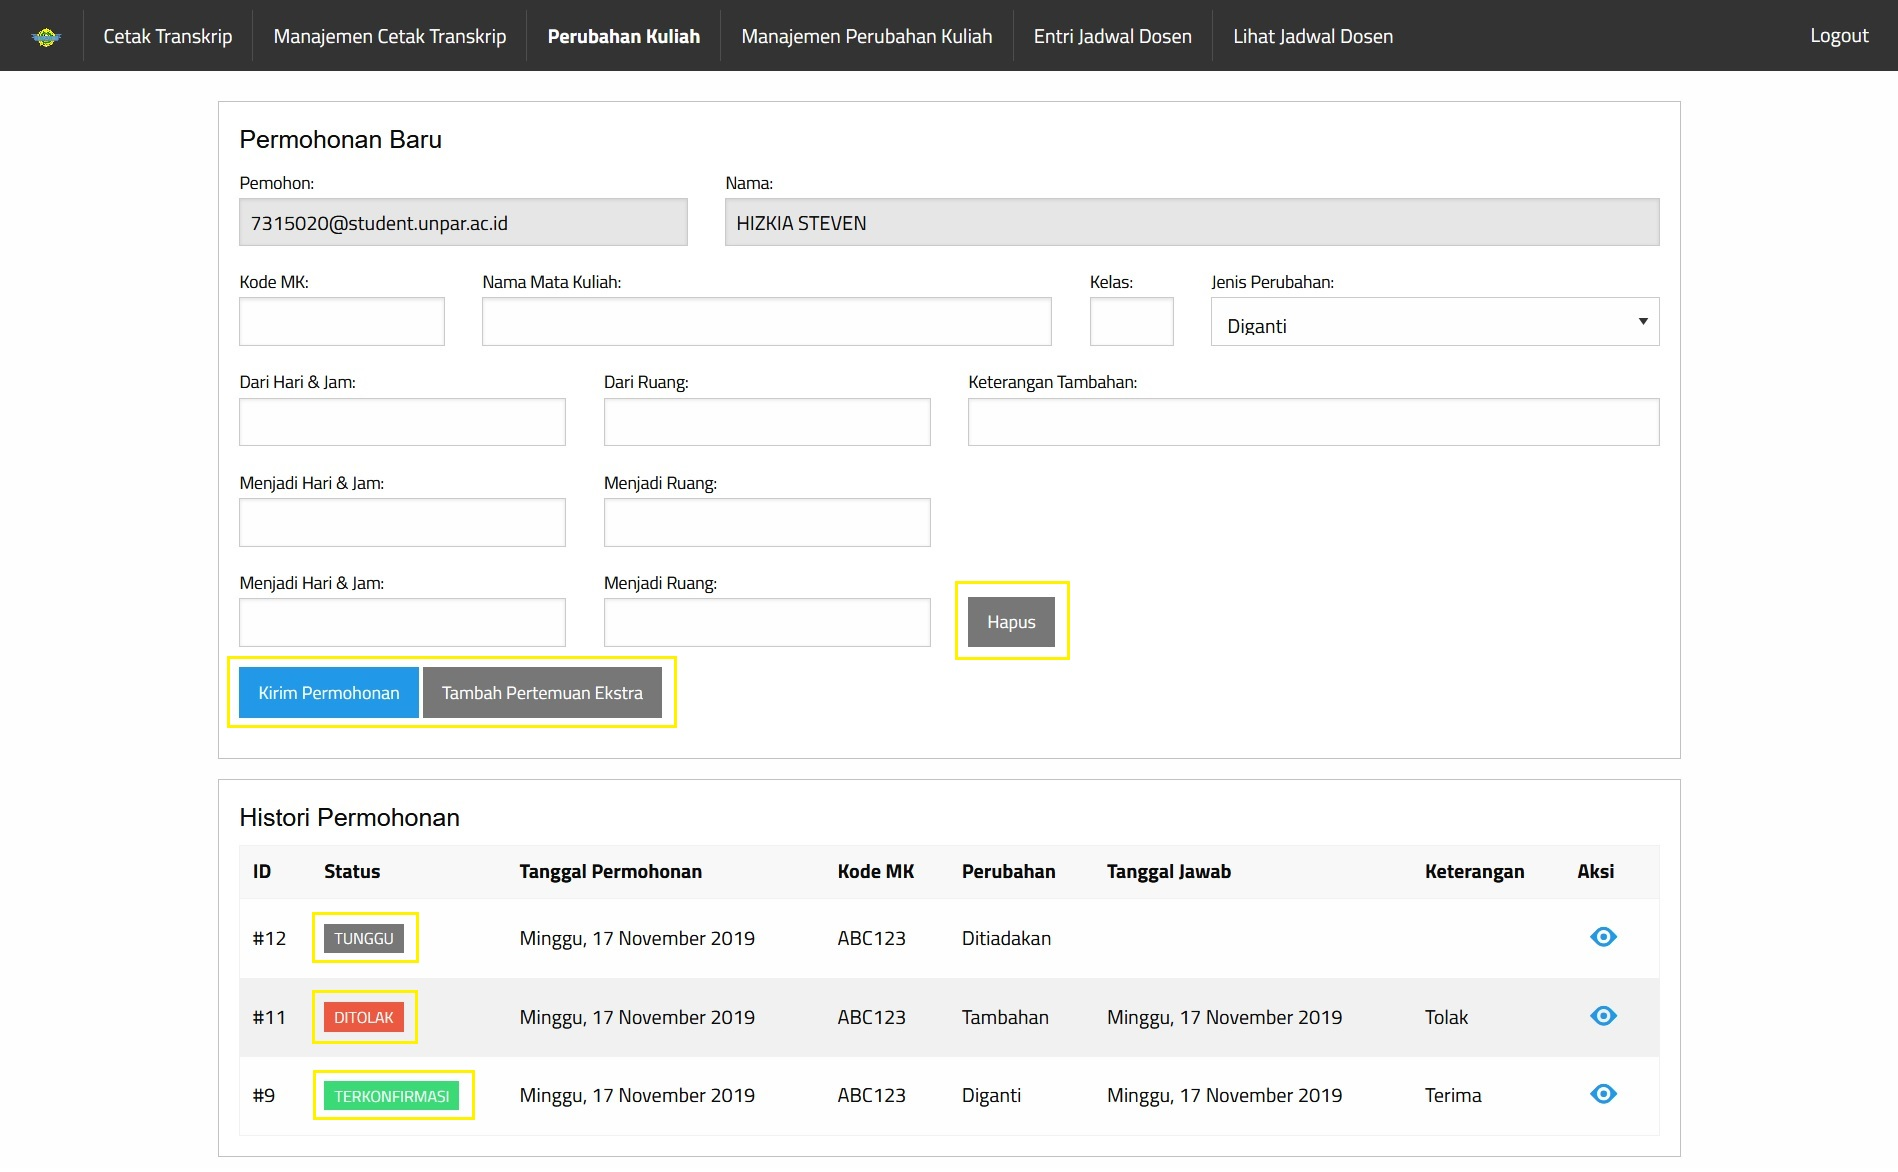
\includegraphics[scale=0.4, frame]{kriteria-sukses-1-4-6-contrast-enchanced-4}  
        \caption[Pelanggaran Kriteria Sukses 1.4.6 pada Halaman Perubahan Kuliah]{Pelanggaran Kriteria Sukses 1.4.6 pada Halaman Perubahan Kuliah}
        \label{fig:1.4.6_contrast_enchanced_4}  
    \end{figure} 
    
    \item Halaman manajemen perubahan kuliah: 
    \begin{itemize}
        \item Teks "Terkonfirmasi" di kolom status pada tabel memiliki rasio kontras 1.79:1 terhadap warna latar belakangnya.
        \item Teks "Menunggu" di kolom status pada tabel memiliki rasio kontras 1.84:1 terhadap warna latar belakangnya.
        \item Teks "Ditolak" di kolom status pada tabel memiliki rasio kontras 3.44:1 terhadap warna latar belakangnya.
        \item Teks "Hapus" pada bagian hapus permohonan memiliki rasio kontras 3.47:1 terhadap warna latar belakangnya.
    \end{itemize}
    Tampilan pada halaman web dapat dilihat pada Gambar \ref{fig:1.4.6_contrast_enchanced_5_1} dan \ref{fig:1.4.6_contrast_enchanced_5_2}. Tautan untuk halaman yang bermasalah dapat dilihat di \url{https://bluetape.azurewebsites.net/PerubahanKuliahManage}.
    \begin{figure}[H]
        \centering  
        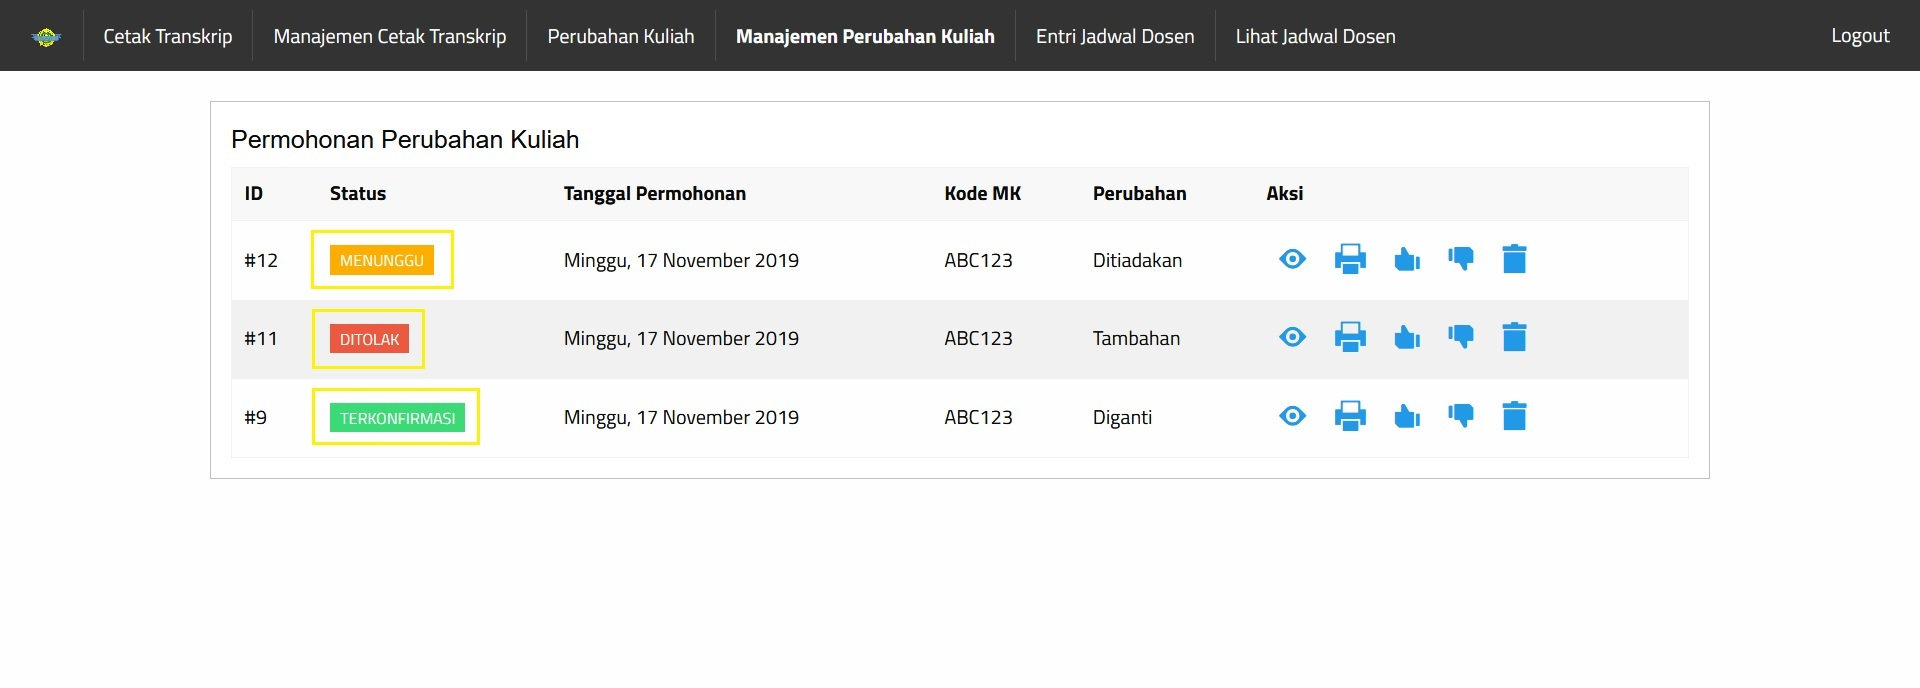
\includegraphics[scale=0.4, frame]{kriteria-sukses-1-4-6-contrast-enchanced-5-1}  
        \caption[Pelanggaran Kriteria Sukses 1.4.6 pada Halaman Manajemen Perubahan Kuliah]{Pelanggaran Kriteria Sukses 1.4.6 pada Halaman Manajemen Perubahan Kuliah}
        \label{fig:1.4.6_contrast_enchanced_5_1}  
    \end{figure} 
    
    \begin{figure}[H]
        \centering  
        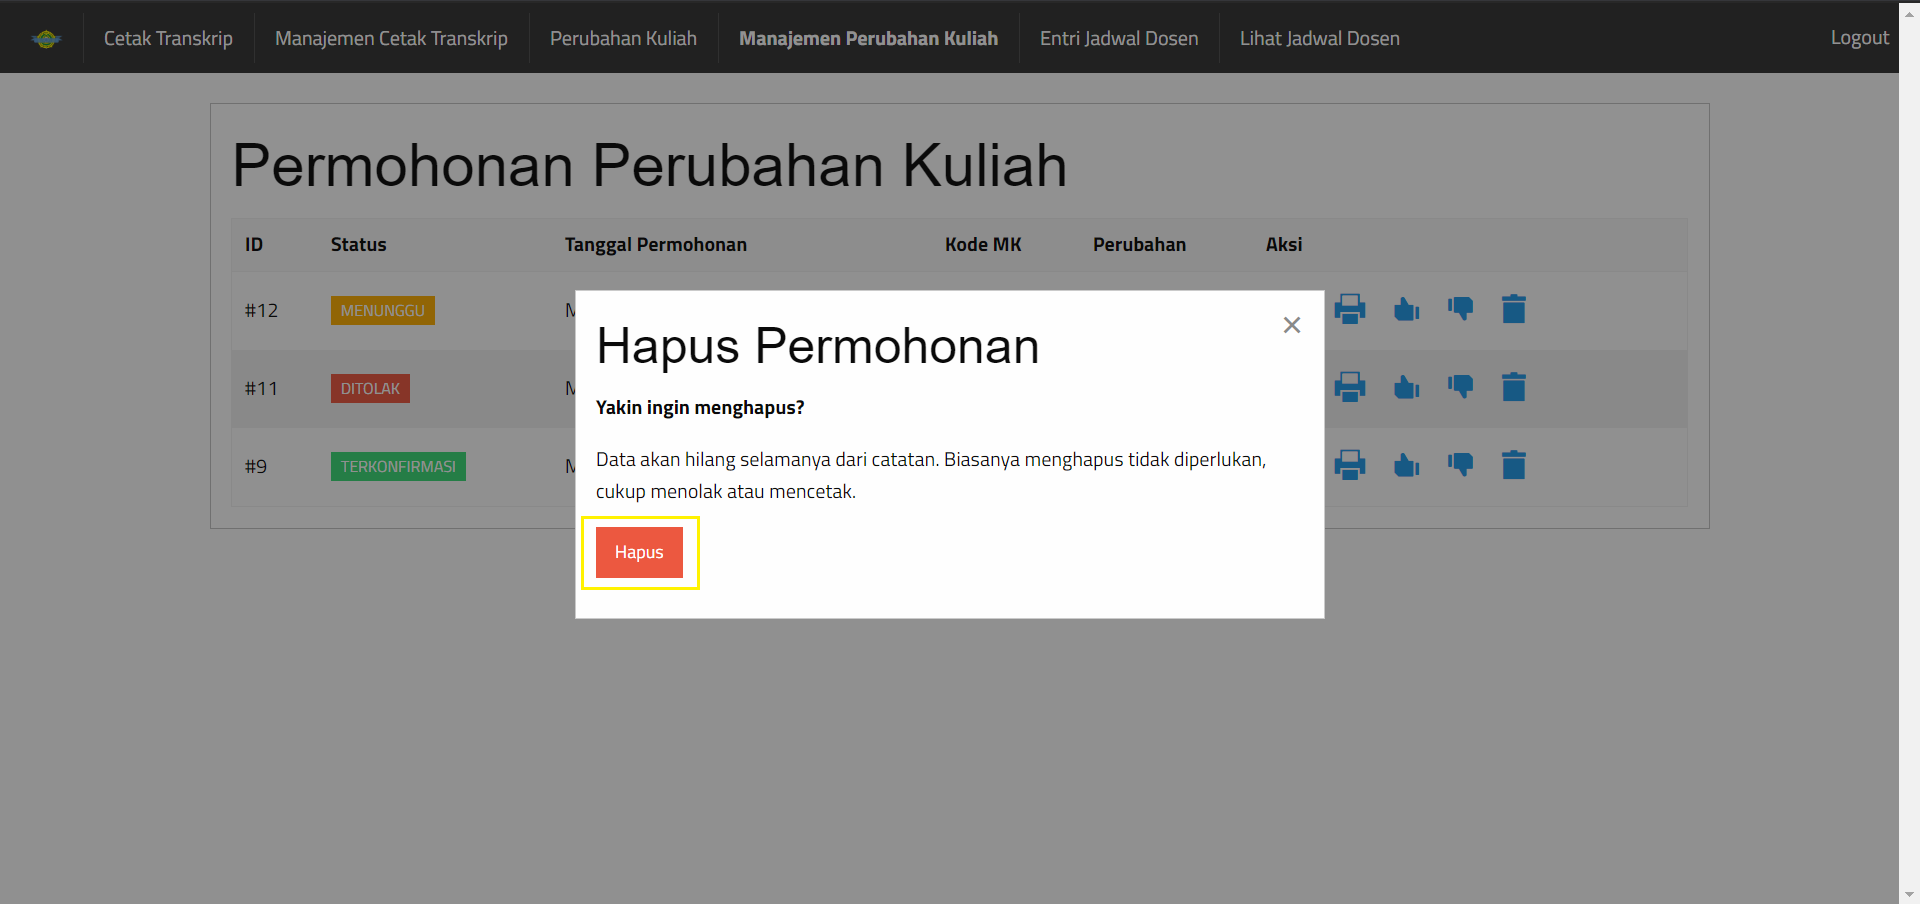
\includegraphics[scale=0.4, frame]{kriteria-sukses-1-4-6-contrast-enchanced-5-2}  
        \caption[Pelanggaran Kriteria Sukses 1.4.6 pada Kotak Dialog di Halaman Manajemen Perubahan Kuliah]{Pelanggaran Kriteria Sukses 1.4.6 pada Kotak Dialog di Halaman Manajemen Perubahan Kuliah}
        \label{fig:1.4.6_contrast_enchanced_5_2}  
    \end{figure}

    \item Halaman entri jadwal dosen: 
    \begin{itemize}
        \item Teks "Tambah" memiliki rasio kontras 3.09:1 terhadap warna latar belakangnya.
        \item Teks "Delete All" memiliki rasio kontras 3.47:1 terhadap warna latar belakangnya.
        \item Teks "Ekspor ke XLS" memiliki rasio kontras 3.09:1 terhadap warna latar belakangnya.
        \item Teks "Save" pada bagian "Edit Jadwal" memiliki rasio kontras 3.09:1 terhadap warna latar belakangnya.
        \item Teks "Delete" memiliki rasio kontras 3.47:1 terhadap warna latar belakangnya.
    \end{itemize}
    Tampilan pada halaman web dapat dilihat pada Gambar \ref{fig:1.4.6_contrast_enchanced_6_1} dan \ref{fig:1.4.6_contrast_enchanced_6_2}. Tautan untuk halaman yang bermasalah dapat dilihat di \url{https://bluetape.azurewebsites.net/EntriJadwalDosen}.
    \begin{figure}[H]
        \centering  
        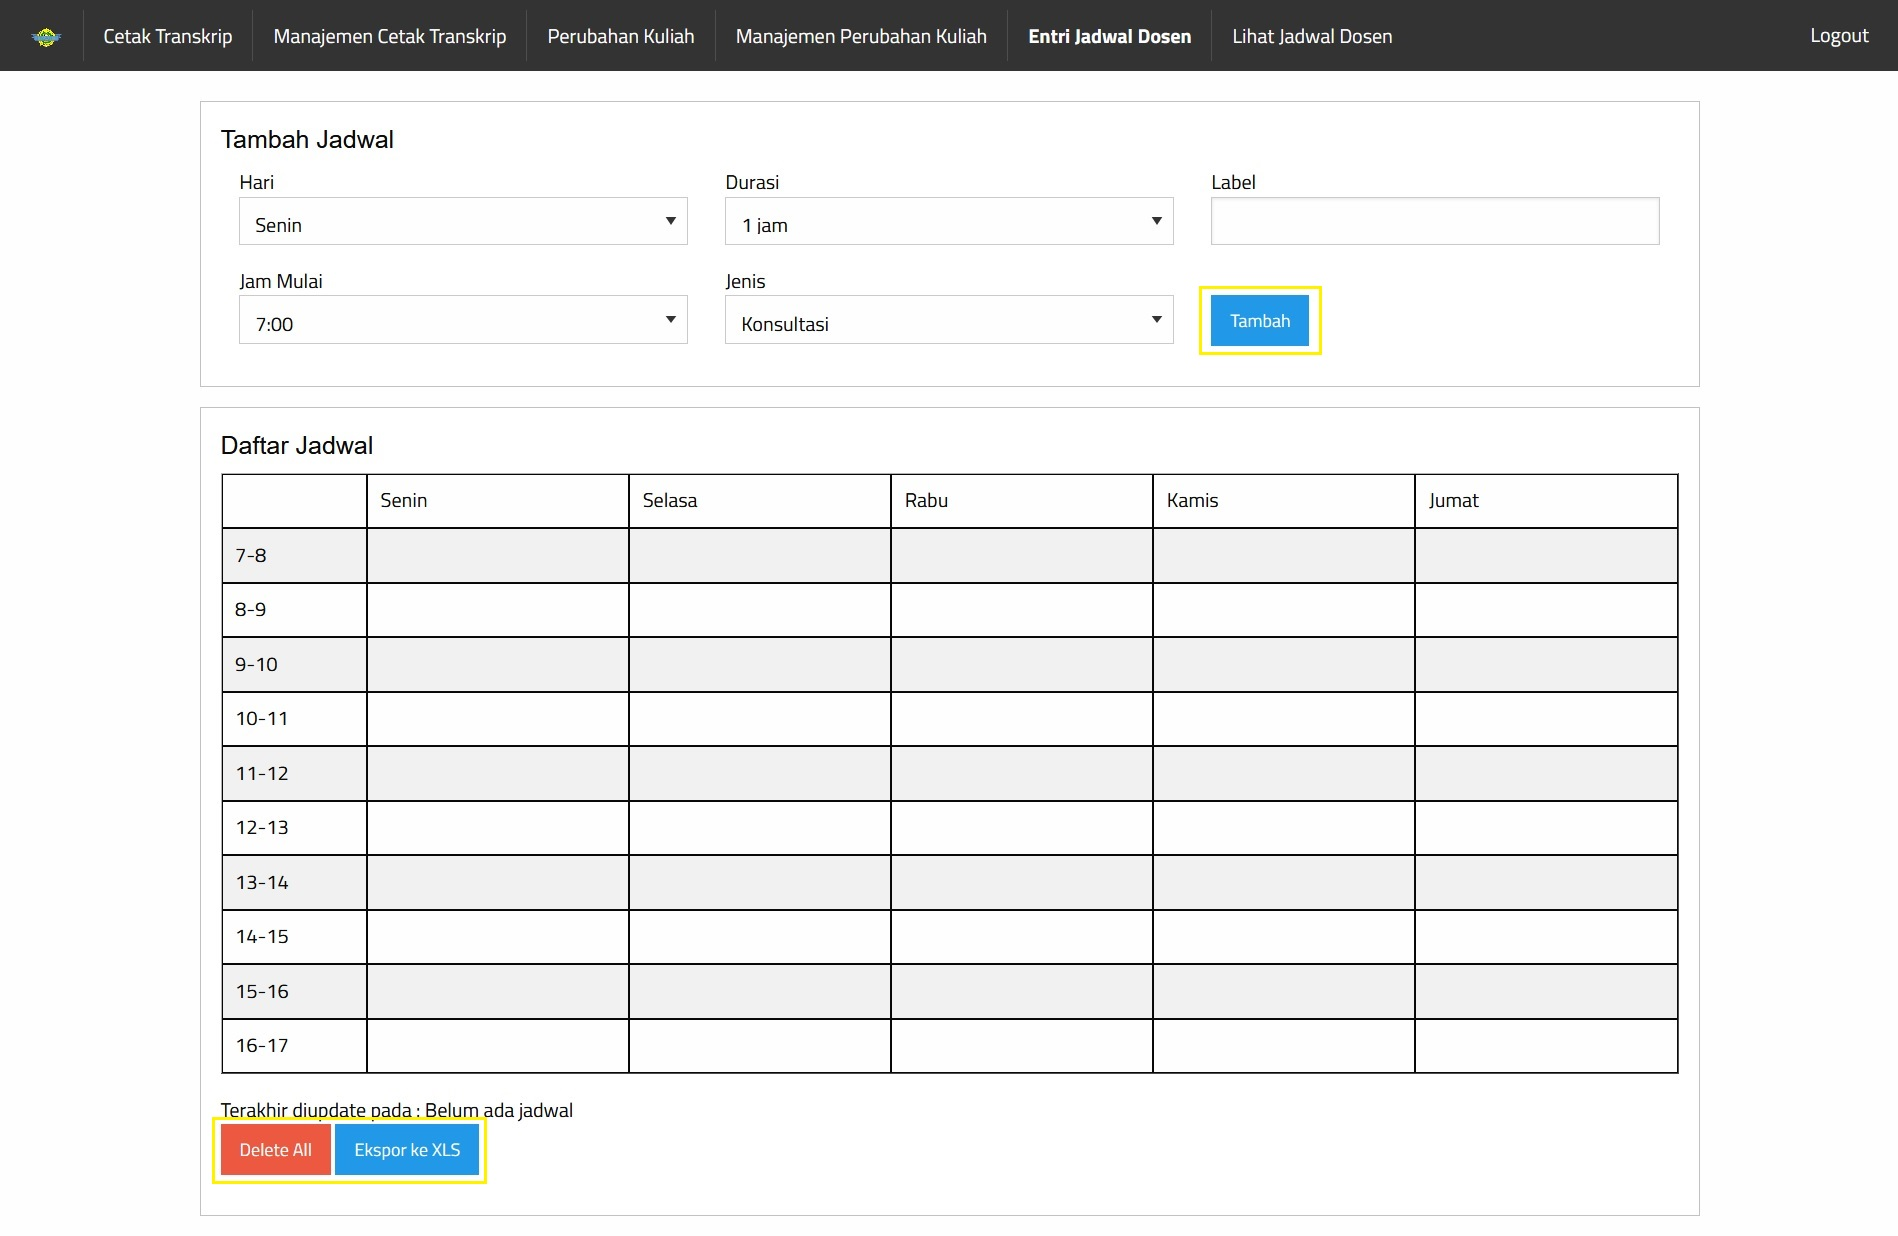
\includegraphics[scale=0.4, frame]{kriteria-sukses-1-4-6-contrast-enchanced-6-1}  
        \caption[Pelanggaran Kriteria Sukses 1.4.6 pada Halaman Entri Jadwal Dosen]{Pelanggaran Kriteria Sukses 1.4.6 pada Halaman Entri Jadwal Dosen}
        \label{fig:1.4.6_contrast_enchanced_6_1}  
    \end{figure} 
    
    \begin{figure}[H]
        \centering  
        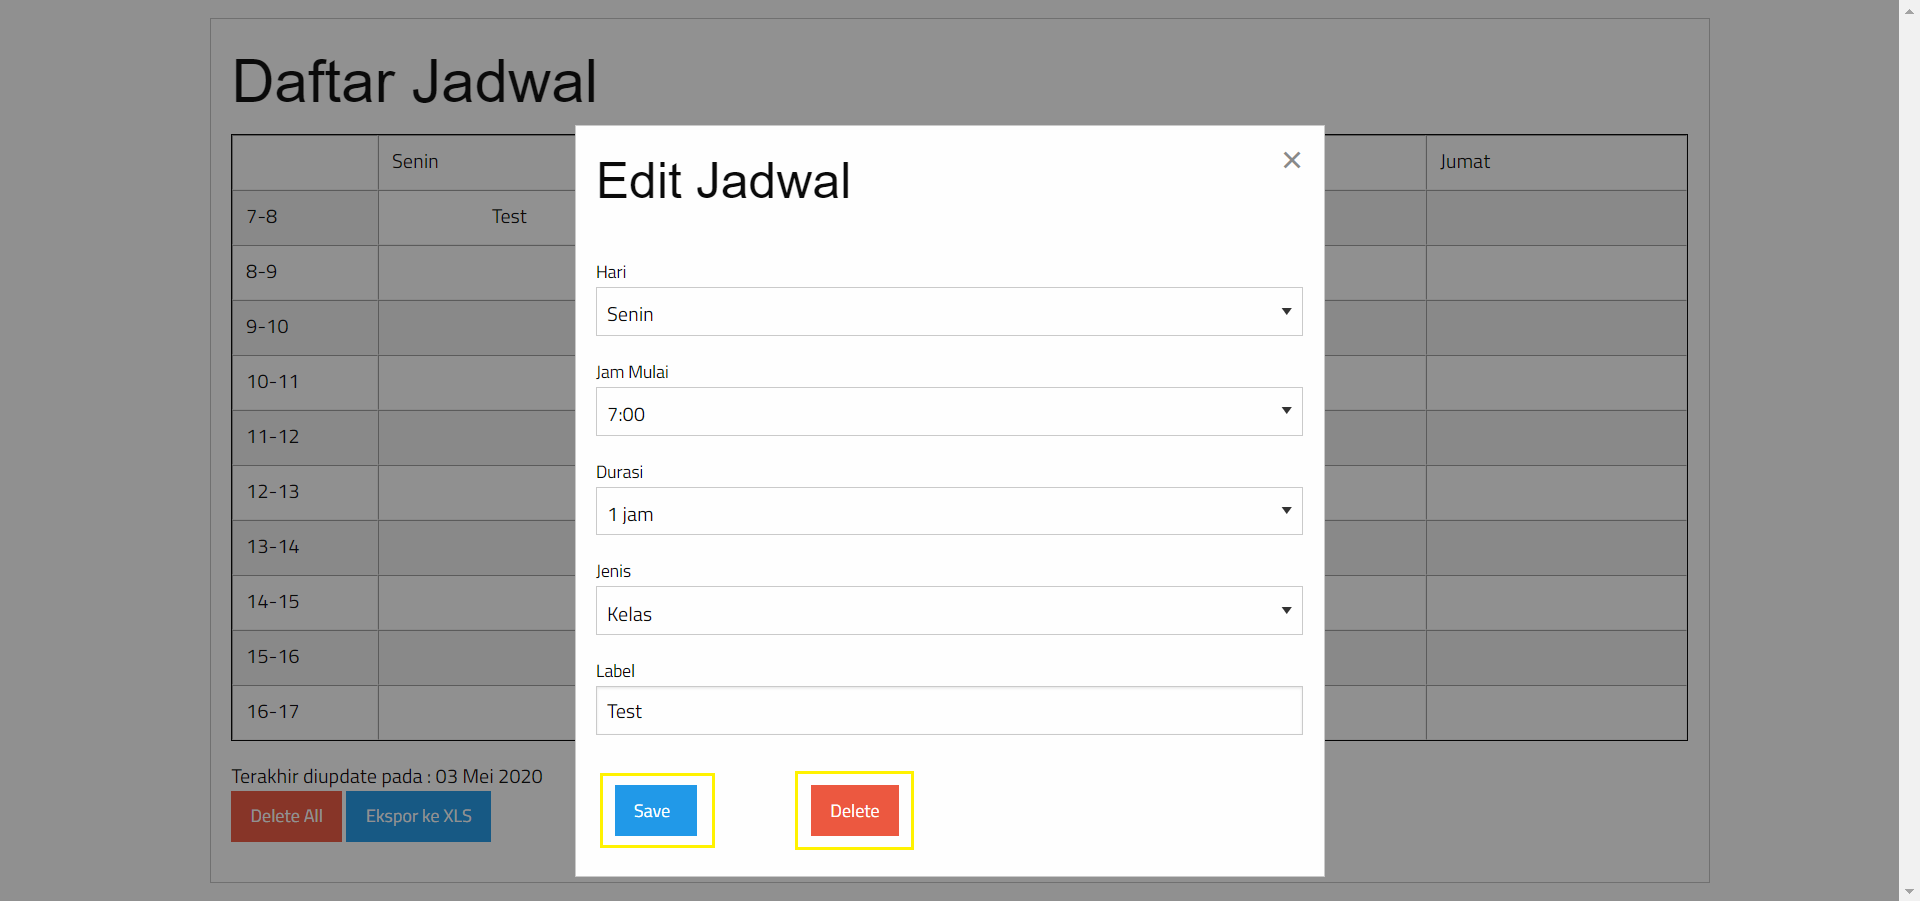
\includegraphics[scale=0.4, frame]{kriteria-sukses-1-4-6-contrast-enchanced-6-2}  
        \caption[Pelanggaran Kriteria Sukses 1.4.6 pada Kotak Dialog di Halaman Entri Jadwal Dosen]{Pelanggaran Kriteria Sukses 1.4.6 pada Kotak Dialog di Halaman Entri Jadwal Dosen}
        \label{fig:1.4.6_contrast_enchanced_6_2}  
    \end{figure} 

    \item Halaman lihat jadwal dosen: 
    \begin{itemize}
        \item Teks nama dosen di atas tabel yang sedang dipilih pengguna memiliki rasio kontras 2.47:1 terhadap warna latar belakangnya.
        \item Teks nama dosen di atas tabel yang sedang tidak dipilih pengguna memiliki rasio kontras 3.06:1 terhadap warna latar belakangnya.
        \item Teks "Ekspor ke XLS" memiliki rasio kontras 3.09:1 terhadap warna latar belakangnya.
    \end{itemize}
    Tampilan pada halaman web dapat dilihat pada Gambar \ref{fig:1.4.6_contrast_enchanced_7}. Tautan untuk halaman yang bermasalah dapat dilihat di \url{https://bluetape.azurewebsites.net/LihatJadwalDosen}.
    \begin{figure}[H]
        \centering  
        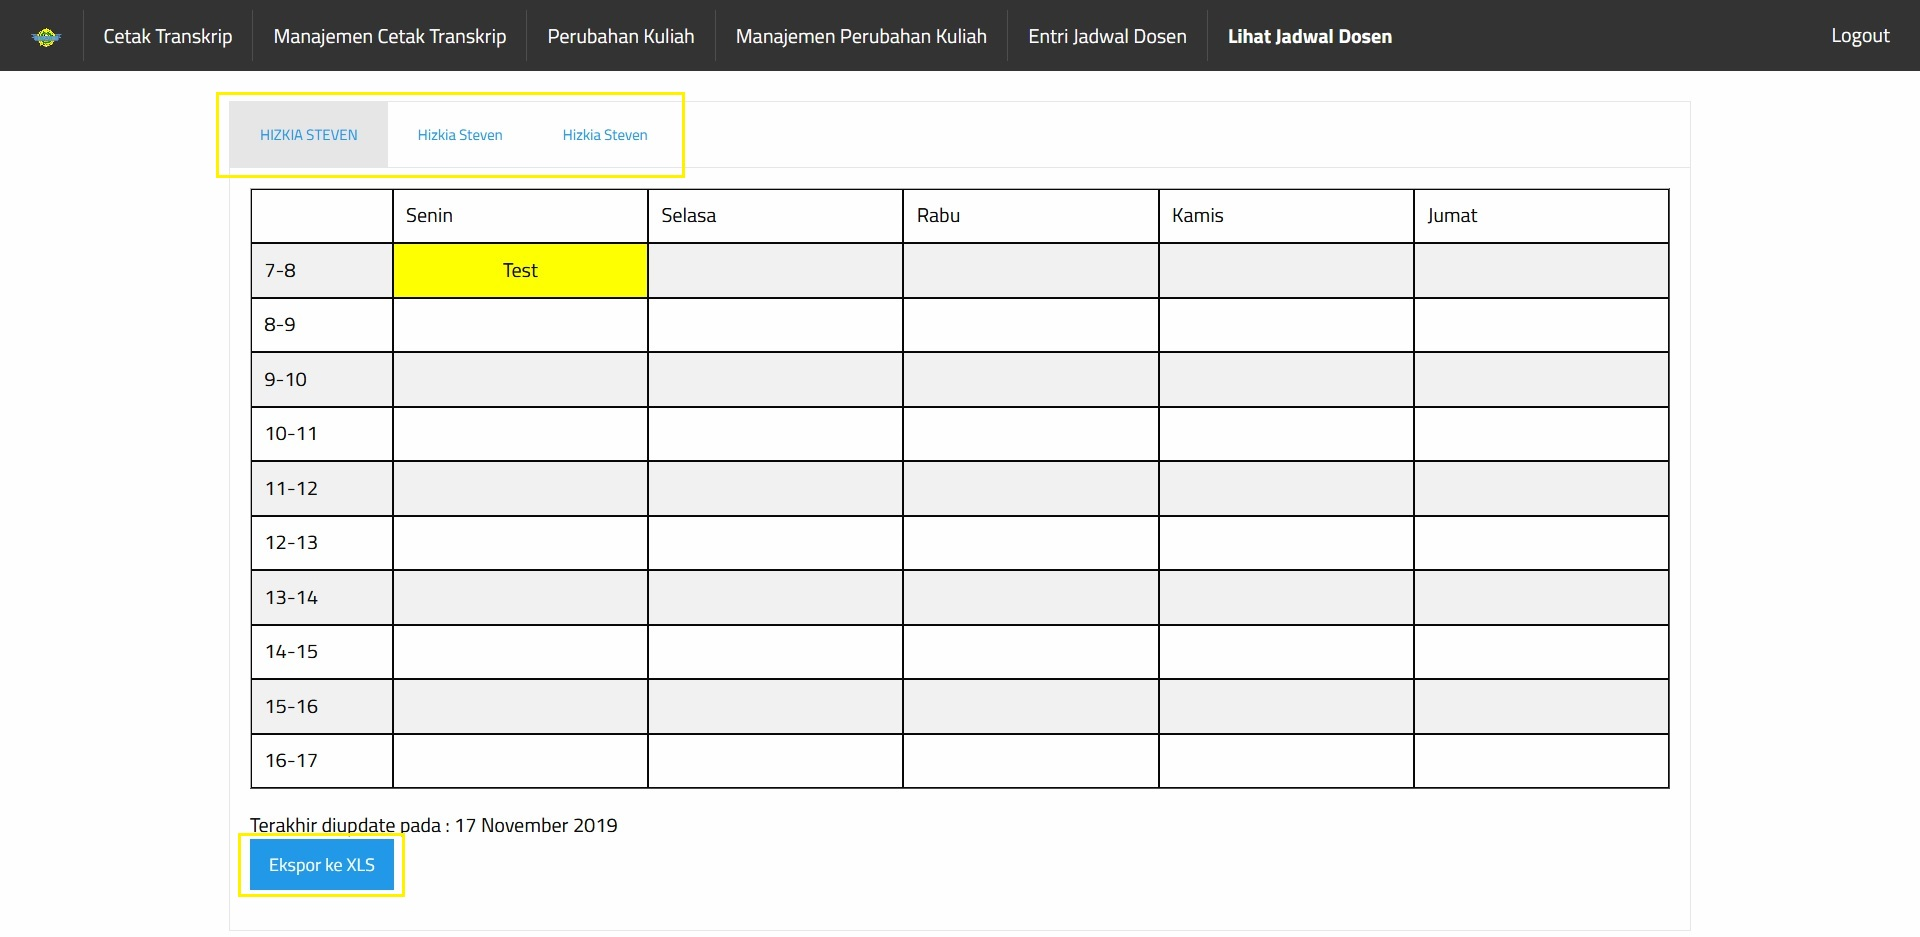
\includegraphics[scale=0.4, frame]{kriteria-sukses-1-4-6-contrast-enchanced-7}  
        \caption[Pelanggaran Kriteria Sukses 1.4.6 pada Halaman Lihat Jadwal Dosen]{Pelanggaran Kriteria Sukses 1.4.6 pada Halaman Lihat Jadwal Dosen}
        \label{fig:1.4.6_contrast_enchanced_7}  
    \end{figure} 
\end{itemize}

\paragraph{Kriteria Sukses 1.4.7 \textit{Low or No Background Audio}}
\label{par:kepatuhan_bluetape_kriteria_sukses_1.4.7}
(Sukses)\\

Kriteria ini sukses dipatuhi karena pada halaman web BlueTape tidak terdapat konten media berbasis waktu.

\paragraph{Kriteria Sukses 1.4.8 \textit{Visual Presentation}}
\label{par:kepatuhan_bluetape_kriteria_sukses_1.4.8}
(Tidak Sukses)\\

Kriteria ini tidak sukses dipatuhi karena pada halaman manajemen cetak transkrip bagian hapus permohonan, teks yang ditampilkan memiliki lebar lebih dari 80 karakter. Tampilan pada halaman web dapat dilihat pada Gambar \ref{fig:1.4.8_visual_presentation}. Tautan untuk halaman yang bermasalah dapat dilihat di \url{https://bluetape.azurewebsites.net/LihatJadwalDosen}.

\begin{figure}[H]
    \centering  
    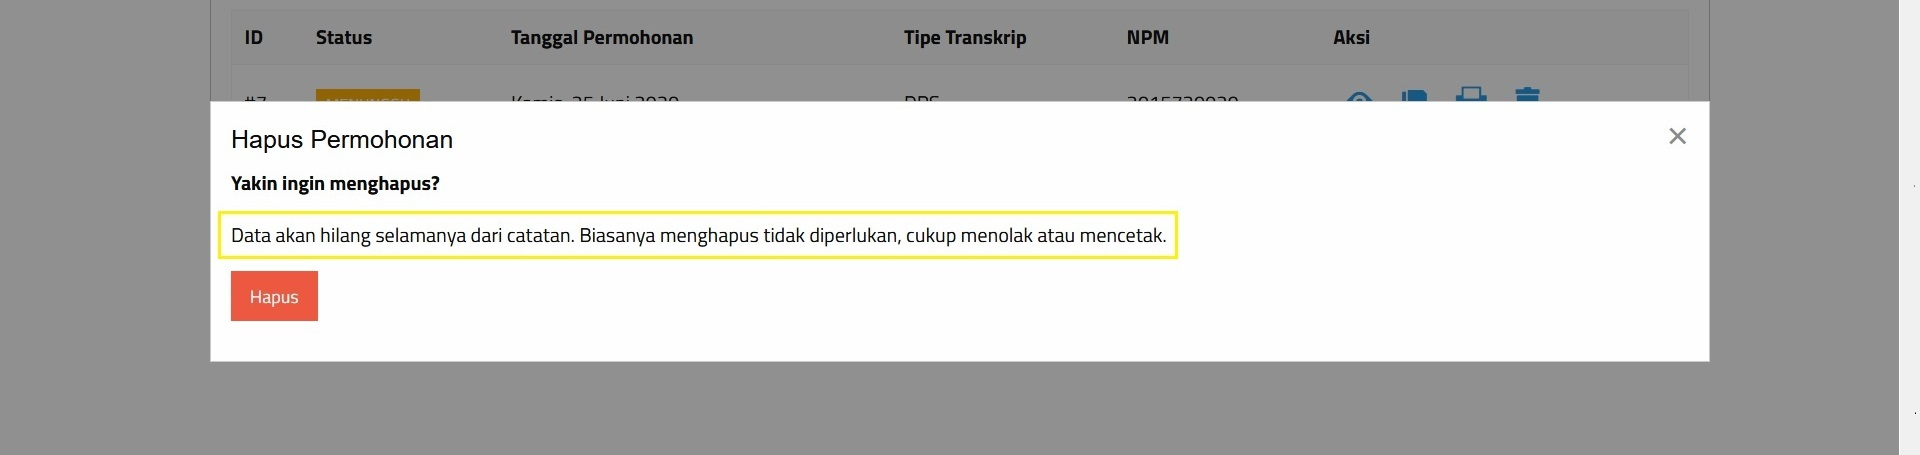
\includegraphics[scale=0.4, frame]{kriteria-sukses-1-4-8-visual-presentation}  
    \caption[Pelanggaran Kriteria Sukses 1.4.8 pada Halaman Manajemen Cetak Transkrip]{Pelanggaran Kriteria Sukses 1.4.8 pada Halaman Manajemen Cetak Transkrip}
    \label{fig:1.4.8_visual_presentation}  
\end{figure} 

\paragraph{Kriteria Sukses 1.4.9 \textit{Images of Text (No Exception)}}
\label{par:kepatuhan_bluetape_kriteria_sukses_1.4.9}
(Sukses)\\

Kriteria ini sukses dipatuhi karena pada halaman web BlueTape tidak terdapat gambar teks selain logo.

\paragraph{Kriteria Sukses 1.4.10 \textit{Reflow}}
\label{par:kepatuhan_bluetape_kriteria_sukses_1.4.10}
(Tidak Sukses)\\

Kriteria ini tidak sukses dipatuhi karena pada halaman web BlueTape, bagian menu navigasi memerlukan \textit{scroll} secara horizontal ketika ditampilkan pada resolusi layar dengan lebar 1280 piksel dan diperbesar hingga 400 persen. Tampilan pada halaman web dapat dilihat pada Gambar \ref{fig:1.4.8_visual_presentation}.

\begin{figure}[H]
    \centering  
    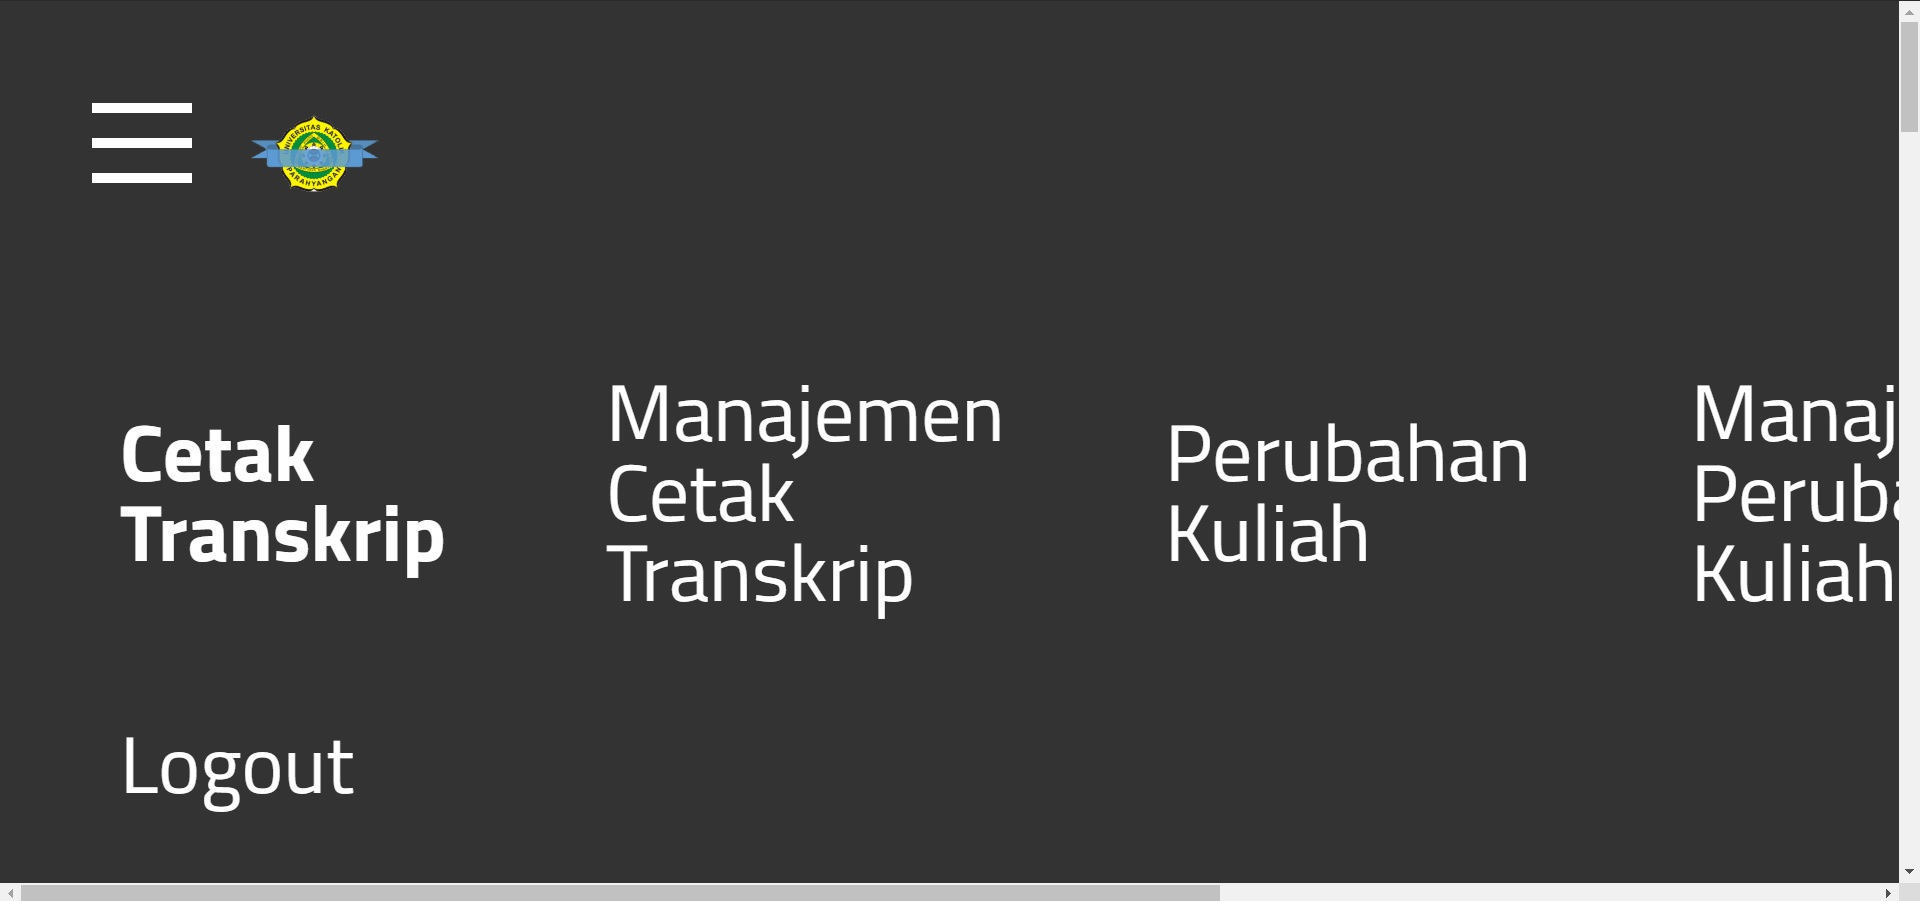
\includegraphics[scale=0.4, frame]{kriteria-sukses-1-4-10-reflow}  
    \caption[Pelanggaran Kriteria Sukses 1.4.10 pada Menu Navigasi]{Pelanggaran Kriteria Sukses 1.4.10 pada Menu Navigasi}
    \label{fig:1.4.10_reflow}  
\end{figure} 

\paragraph{Kriteria Sukses 1.4.11 \textit{Non-text Contrast}}
\label{par:kepatuhan_bluetape_kriteria_sukses_1.4.11}
(Sukses)\\

Kriteria ini sukses dipatuhi karena pada halaman web BlueTape setiap objek grafis yang berupa ikon sudah memiliki rasio kontras lebih dari 3:1 terhadap warna yang berdekatan.

\paragraph{Kriteria Sukses 1.4.12 \textit{Text Spacing}}
\label{par:kepatuhan_bluetape_kriteria_sukses_1.4.12}
(Sukses)\\

Kriteria ini sukses dipatuhi karena penulis sudah melakukan uji coba dengan mengubah beberapa bagian pada halaman perubahan kuliah sesuai kriteria ini dan tidak terjadi masalah. Oleh karena itu, penulis menduga tidak akan ada masalah ketika ukuran-ukuran tertentu diubah pada halaman lain. Tampilan pada halaman web dapat dilihat pada Gambar \ref{fig:1.4.12_text_spacing}.

\begin{figure}[H]
    \centering  
    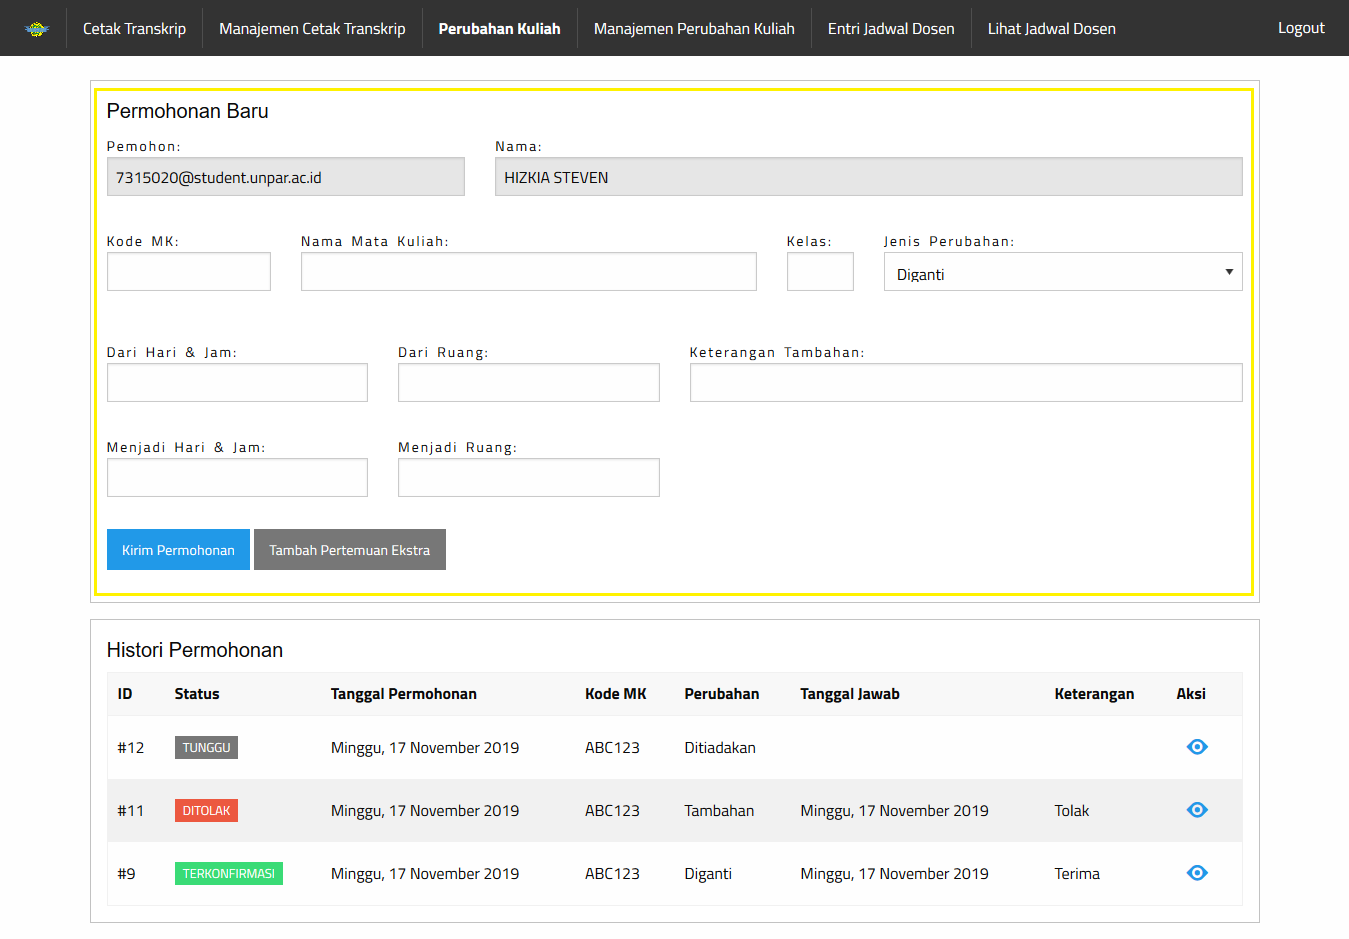
\includegraphics[scale=0.4, frame]{kriteria-sukses-1-4-12-text-spacing}  
    \caption[Kesuksesan Kriteria Sukses 1.4.12 pada Halaman Perubahan Kuliah]{Kesuksesan Kriteria Sukses 1.4.12 pada Halaman Perubahan Kuliah}
    \label{fig:1.4.12_text_spacing}  
\end{figure} 

\paragraph{Kriteria Sukses 1.4.13 \textit{Content on Hover or Focus}}
\label{par:kepatuhan_bluetape_kriteria_sukses_1.4.13}
(Sukses)\\

Kriteria ini sukses dipatuhi karena setiap konten tambahan yang muncul ketika suatu elemen menerima kursor atau fokus \textit{keyboard}, konten tambahan tersebut dapat disingkirkan, kursor dapat dipindahkan ke konten tambahan tanpa membuat konten tambahan tersebut menghilang, dan konten tambahan tetap tampak sampai penunjuk atau pemicu fokus dihapus.

\subsection{\textit{Operable}}
\label{subsec:kepatuhan_bluetape_operable}
Pada subbab ini dibahas kriteria-kriteria sukses yang termasuk ke dalam kategori \textit{operable}. Hasil sukses atau tidaknya aplikasi BlueTape terhadap poin-poin kriteria sukses dalam kategori ini ditampilkan pada Tabel \ref{tab:kepatuhan_bluetape_operable}.

\begin{table}[H]
    \centering 
    \caption{Kepatuhan BlueTape terhadap prinsip \textit{Operable}}
    \label{tab:kepatuhan_bluetape_operable}
    \begin{tabular}{|c|c|c|}
        \toprule
        Kriteria Sukses & Hasil (sukses/tidak) & Tingkat Kepatuhan\\

        \midrule
        \rowcolor{darkred} 2.1.1 & Tidak Sukses & A \\
        2.1.2 & Sukses & A \\
        \rowcolor{pink} 2.1.3 & Tidak Sukses & AAA \\
        2.1.4 & Sukses & A \\
        2.2.1 & Sukses & A \\
        2.2.2 & Sukses & A \\
        2.2.3 & Sukses & AAA \\
        2.2.4 & Sukses & AAA \\
        \rowcolor{pink} 2.2.5 & Tidak Sukses & AAA \\
        \rowcolor{pink} 2.2.6 & Tidak Sukses & AAA \\
        2.3.1 & Sukses & A \\
        2.3.2 & Sukses & AAA \\
        2.3.3 & Sukses & AAA \\
        \rowcolor{darkred} 2.4.1 & Tidak Sukses & A \\
        2.4.2 & Sukses & A \\
        2.4.3 & Sukses & A \\
        \rowcolor{darkred} 2.4.4 & Tidak Sukses & A \\
        \rowcolor{brightred} 2.4.5 & Tidak Sukses & AA \\
        \rowcolor{brightred} 2.4.6 & Tidak Sukses & AA \\
        \rowcolor{brightred} 2.4.7 & Tidak Sukses & AA \\
        2.4.8 & Sukses & AAA \\
        \rowcolor{pink} 2.4.9 & Tidak Sukses & AAA \\
        \rowcolor{pink} 2.4.10 & Tidak Sukses & AAA \\
        2.5.1 & Sukses & A \\
        2.5.2 & Sukses & A \\
        \rowcolor{darkred} 2.5.3 & Tidak Sukses & A \\
        2.5.4 & Sukses & A \\
        \rowcolor{pink} 2.5.5 & Tidak Sukses & AAA \\
        2.5.6 & Sukses & AAA \\

        \bottomrule
        \multicolumn{2}{|c|}{Tingkat kepatuhan tertinggi yang dicapai} & - \\
        \bottomrule

    \end{tabular}
\end{table}

\subsubsection{\textit{Keyboard Accessible}}
\label{subsubsec:kepatuhan_bluetape_keyboard_accessible}
Pada subbab ini dibahas alasan mengapa poin kriteria sukses pada kategori \textit{keyboard accessible} dinilai sukses atau tidak sukses.

\paragraph{Kriteria Sukses 2.1.1 \textit{Keyboard}}
\label{par:kepatuhan_bluetape_kriteria_sukses_2.1.1}
(Tidak Sukses)\\

Kriteria ini tidak sukses dipatuhi karena terdapat fungsionalitas konten yang tidak dapat dioperasikan melalui \textit{keyboard}, antara lain:

\begin{itemize}
    \item Pada bagian menu navigasi, pengguna tidak dapat memilih halaman yang diinginkan. Tampilan pada halaman web dapat dilihat pada Gambar \ref{fig:2.1.1_keyboard_1}.
    \begin{figure}[H]
        \centering  
        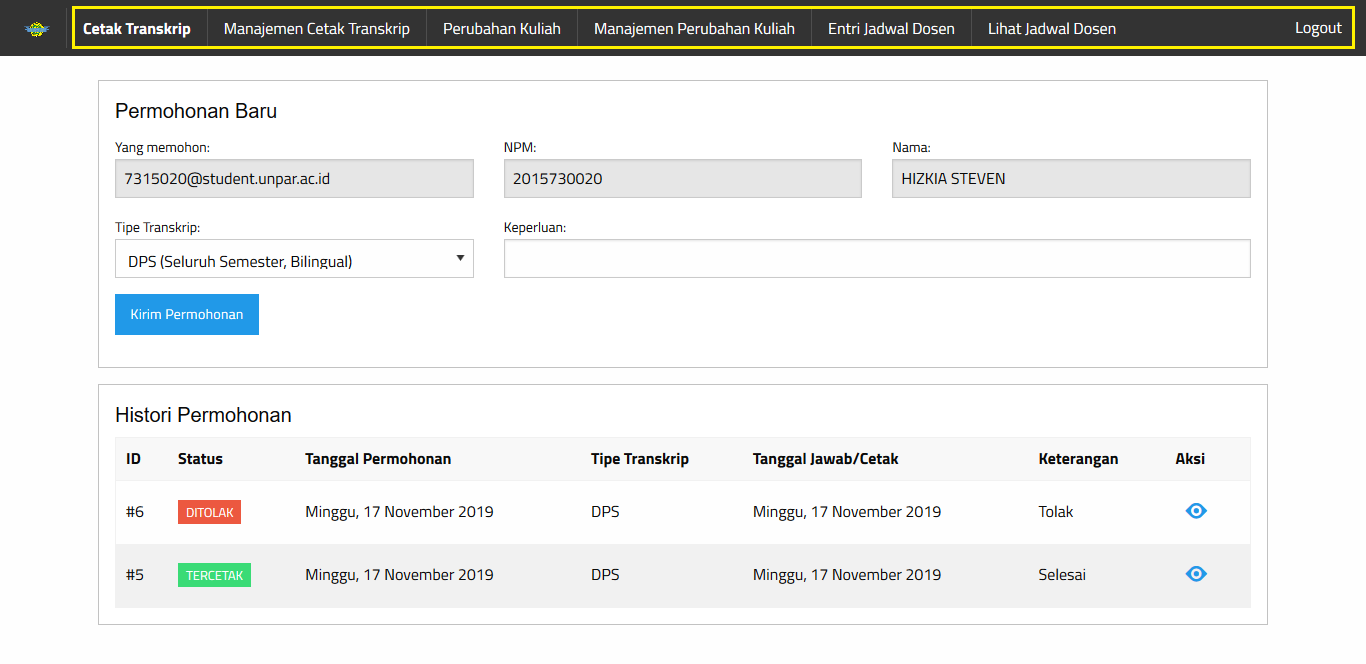
\includegraphics[scale=0.4, frame]{kriteria-sukses-2-1-1-keyboard-1}  
        \caption[Pelanggaran Kriteria Sukses 2.1.1 pada Menu Navigasi]{Pelanggaran Kriteria Sukses 2.1.1 pada Menu Navigasi}
        \label{fig:2.1.1_keyboard_1}  
    \end{figure} 

    \item Pada bagian tabel "Daftar Jadwal" di halaman entri jadwal dosen. Tampilan pada halaman web dapat dilihat pada Gambar \ref{fig:2.1.1_keyboard_2}. Tautan untuk halaman yang bermasalah dapat dilihat di \url{https://bluetape.azurewebsites.net/EntriJadwalDosen}.
    \begin{figure}[H]
        \centering  
        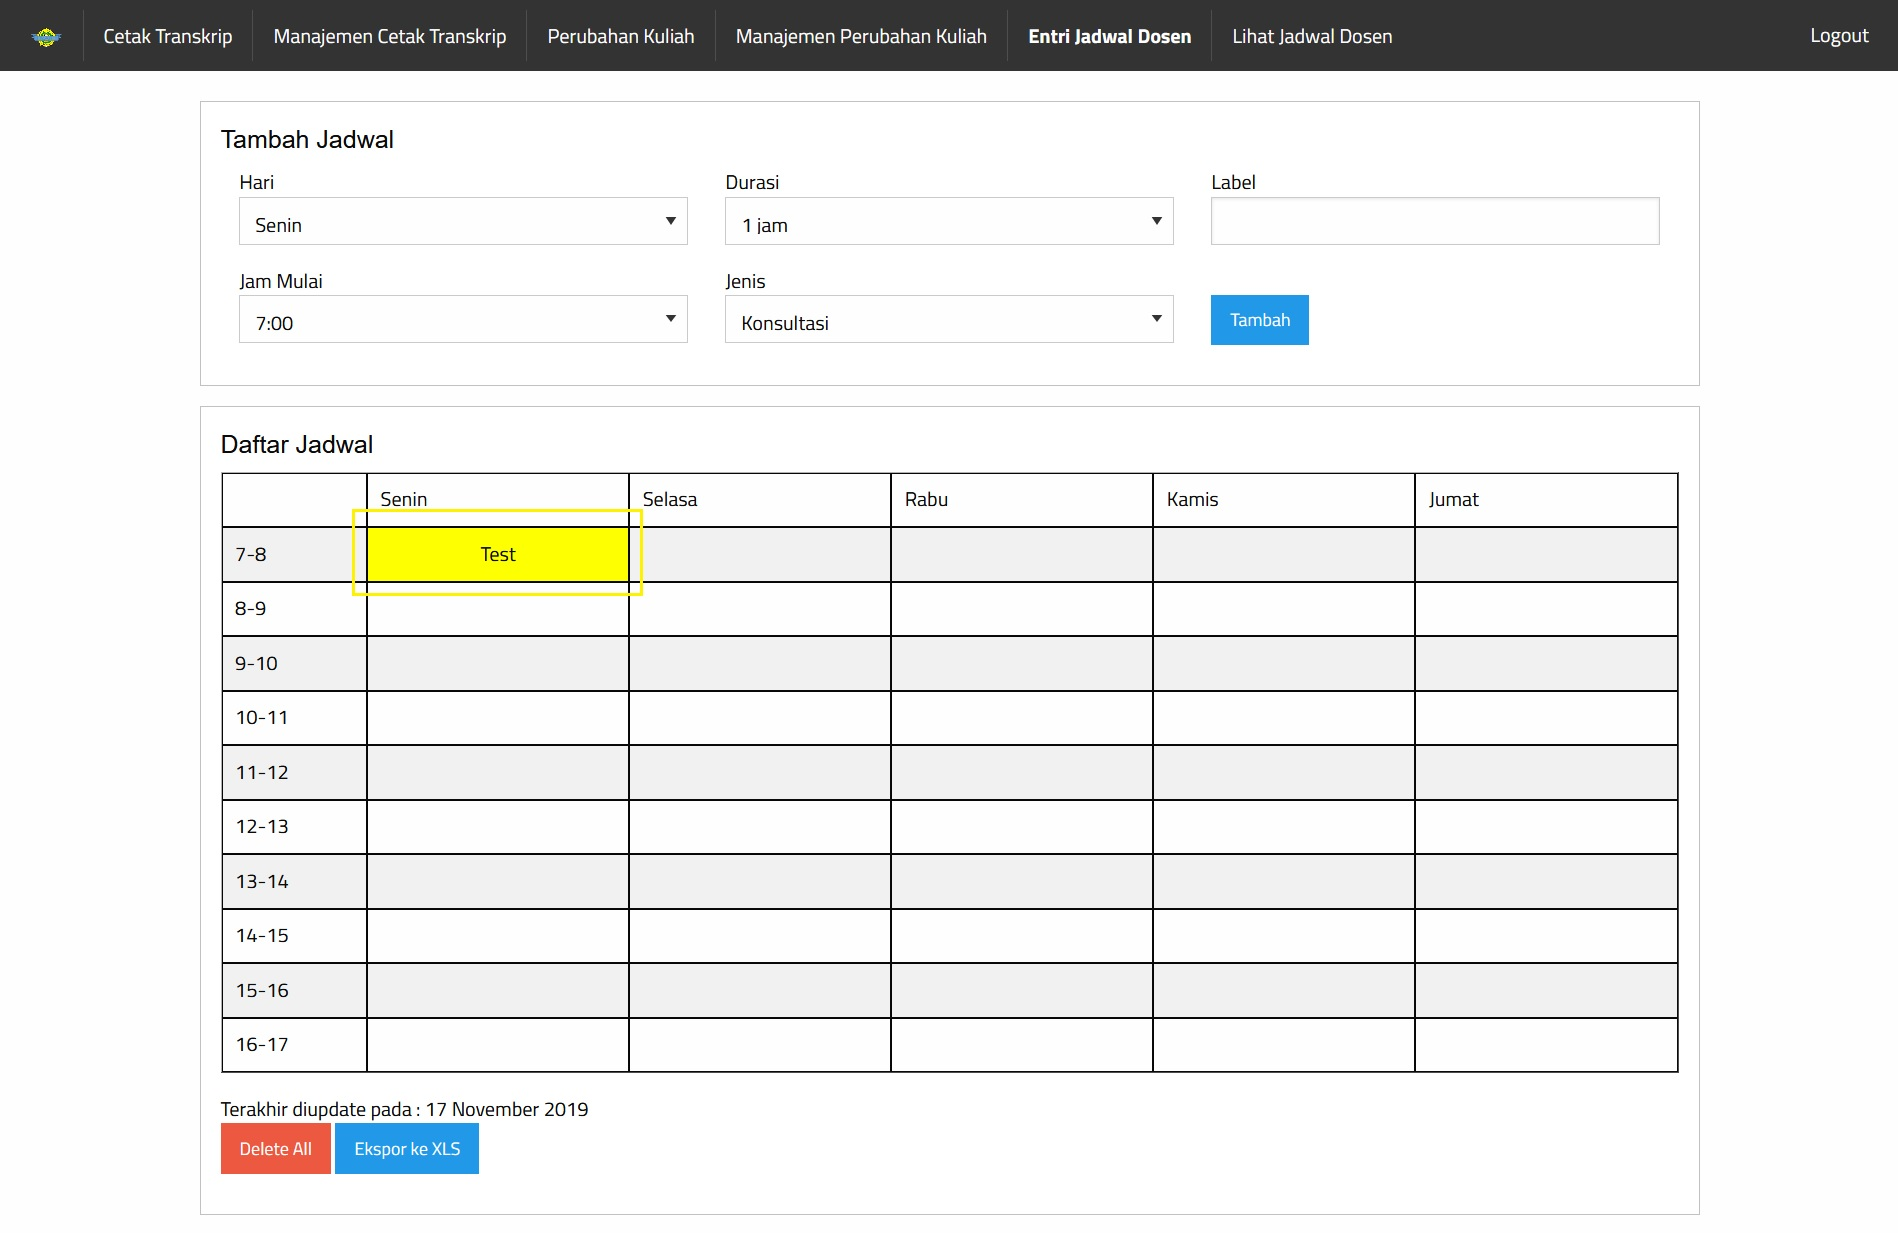
\includegraphics[scale=0.4, frame]{kriteria-sukses-2-1-1-keyboard-2}  
        \caption[Pelanggaran Kriteria Sukses 2.1.1 pada Halaman Entri Jadwal Dosen]{Pelanggaran Kriteria Sukses 2.1.1 pada Halaman Entri Jadwal Dosen}
        \label{fig:2.1.1_keyboard_2}  
    \end{figure} 
\end{itemize}

\paragraph{Kriteria Sukses 2.1.2 \textit{No Keyboard Trap}}
\label{par:kepatuhan_bluetape_kriteria_sukses_2.1.2}
(Sukses)\\

Kriteria ini sukses dipatuhi karena pengguna dapat bernavigasi dari satu komponen ke komponen lain pada setiap komponen yang dapat dinavigasikan pada halaman web BlueTape dengan menggunakan \textit{keyboard} tanpa terperangkap dalam suatu komponen tertentu.

\paragraph{Kriteria Sukses 2.1.3 \textit{Keyboard (No Exception)}}
\label{par:kepatuhan_bluetape_kriteria_sukses_2.1.3}
(Tidak Sukses)\\

Kriteria ini tidak sukses dipatuhi karena terdapat fungsionalitas konten yang tidak dapat dioperasikan melalui \textit{keyboard}, antara lain:

\begin{itemize}
    \item Pada bagian menu navigasi, pengguna tidak dapat memilih halaman yang diinginkan. Tampilan pada halaman web dapat dilihat pada Gambar \ref{fig:2.1.3_keyboard_no_exception_1}.
    \begin{figure}[H]
        \centering  
        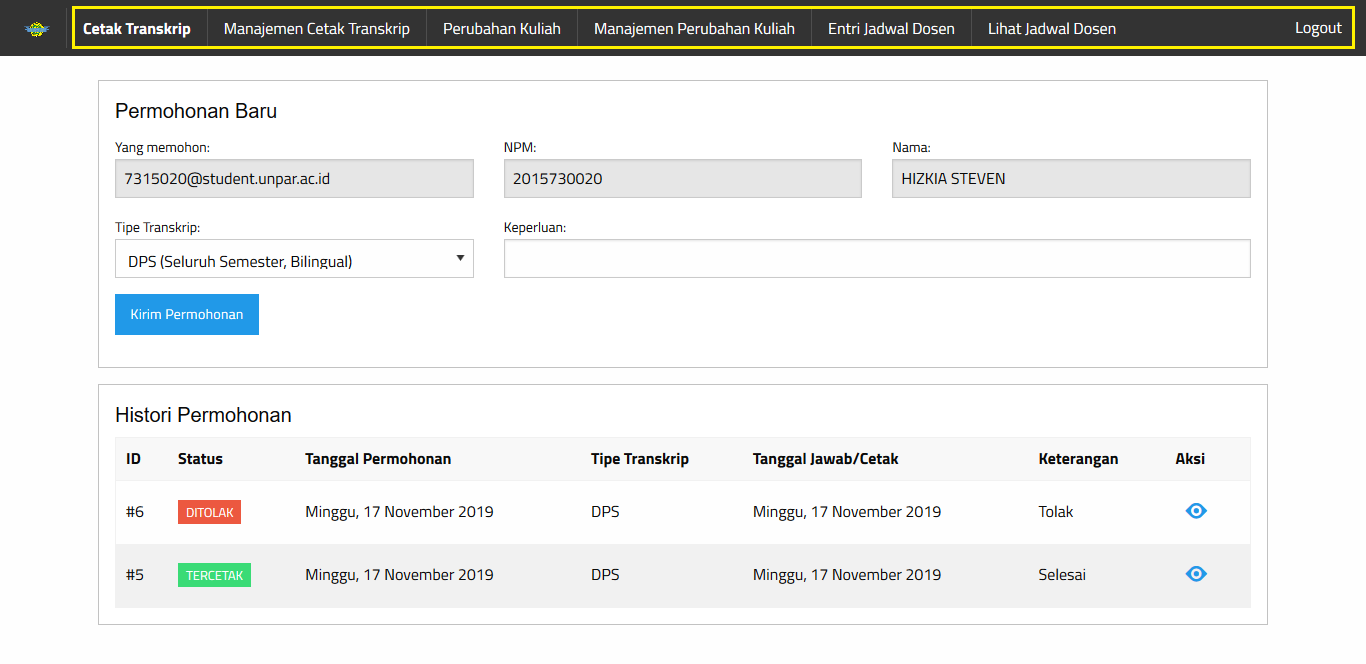
\includegraphics[scale=0.4, frame]{kriteria-sukses-2-1-3-keyboard-no-exception-1}  
        \caption[Pelanggaran Kriteria Sukses 2.1.3 pada Menu Navigasi]{Pelanggaran Kriteria Sukses 2.1.3 pada Menu Navigasi}
        \label{fig:2.1.3_keyboard_no_exception_1}  
    \end{figure} 

    \item Pada bagian tabel "Daftar Jadwal" di halaman entri jadwal dosen. Tampilan pada halaman web dapat dilihat pada Gambar \ref{fig:2.1.3_keyboard_no_exception_2}. Tautan untuk halaman yang bermasalah dapat dilihat di \url{https://bluetape.azurewebsites.net/EntriJadwalDosen}.
    \begin{figure}[H]
        \centering  
        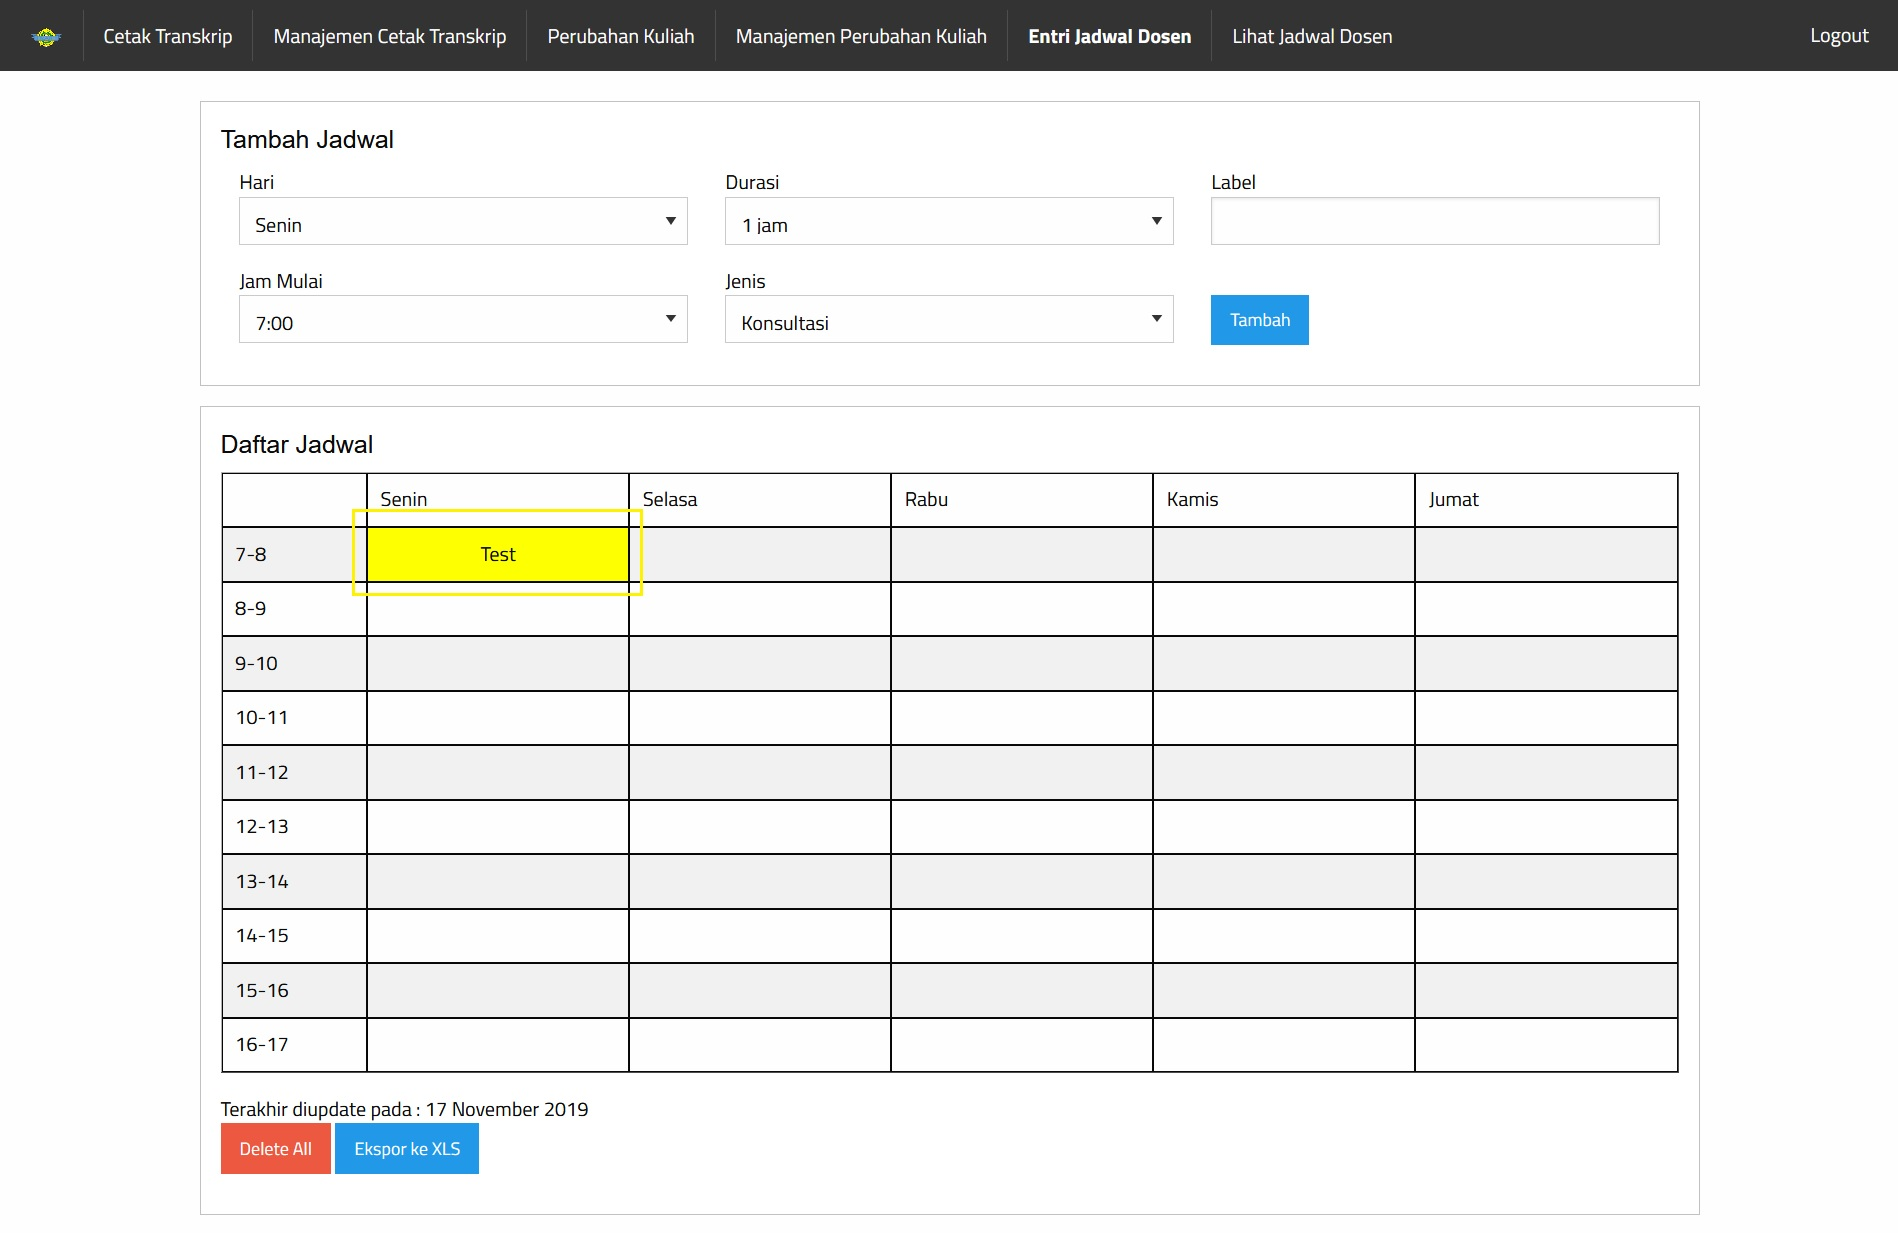
\includegraphics[scale=0.4, frame]{kriteria-sukses-2-1-3-keyboard-no-exception-2}  
        \caption[Pelanggaran Kriteria Sukses 2.1.3 pada Halaman Entri Jadwal Dosen]{Pelanggaran Kriteria Sukses 2.1.3 pada Halaman Entri Jadwal Dosen}
        \label{fig:2.1.3_keyboard_no_exception_2}  
    \end{figure} 
\end{itemize}

\paragraph{Kriteria Sukses 2.1.4 \textit{Character Key Shortcuts}}
\label{par:kepatuhan_bluetape_kriteria_sukses_2.1.4}
(Sukses)\\

Kriteria ini sukses dipatuhi karena pada halaman web BlueTape tidak terdapat pintasan \textit{keyboard} untuk konten yang disajikan.

\subsubsection{\textit{Enough Time}}
\label{subsubsec:kepatuhan_bluetape_enough_time}
Pada subbab ini dibahas alasan mengapa poin kriteria sukses pada kategori \textit{enough time} dinilai sukses atau tidak sukses.

\paragraph{Kriteria Sukses 2.2.1 \textit{Timing Adjustable}}
\label{par:kepatuhan_bluetape_kriteria_sukses_2.2.1}
(Sukses)\\

Kriteria ini sukses dipatuhi karena pada halaman web BlueTape tidak terdapat batas waktu bagi pengguna untuk membaca dan memanfaatkan konten.

\paragraph{Kriteria Sukses 2.2.2 \textit{Pause, Stop, Hide}}
\label{par:kepatuhan_bluetape_kriteria_sukses_2.2.2}
(Sukses)\\

Kriteria ini sukses dipatuhi karena pada halaman web BlueTape tidak terdapat konten yang bergerak, berkelip, bergulir, ataupun diperbarui otomatis.

\paragraph{Kriteria Sukses 2.2.3 \textit{No Timing}}
\label{par:kepatuhan_bluetape_kriteria_sukses_2.2.3}
(Sukses)\\

Kriteria ini sukses dipatuhi karena pada halaman web BlueTape tidak terdapat batas waktu bagi pengguna untuk membaca dan memanfaatkan konten.

\paragraph{Kriteria Sukses 2.2.4 \textit{Interruptions}}
\label{par:kepatuhan_bluetape_kriteria_sukses_2.2.4}
(Sukses)\\

Kriteria ini sukses dipatuhi karena setiap interupsi pada halaman web BlueTape dapat ditunda atau dihentikan oleh pengguna.

\paragraph{Kriteria Sukses 2.2.5 \textit{Re-authenticating}}
\label{par:kepatuhan_bluetape_kriteria_sukses_2.2.5}
(Tidak Sukses)\\

Kriteria ini tidak sukses dipatuhi karena ketika pengguna akan mengirim data dan sesi otentikasi berakhir, pengguna kehilangan data tersebut setelah melakukan otentikasi ulang.

\paragraph{Kriteria Sukses 2.2.6 \textit{Timeouts}}
\label{par:kepatuhan_bluetape_kriteria_sukses_2.2.6}
(Tidak Sukses)\\

Kriteria ini tidak sukses dipatuhi karena tidak terdapat peringatan untuk pengguna ketika sesi otentikasi akan berakhir yang dapat menyebabkan kehilangan data. Data pengguna tidak disimpan untuk bertahan lebih dari 20 jam ketika pengguna tidak melakukan tindakan apa pun. Pada \textit{Listing} \ref{lst:2.2.6_sesi_otentikasi} ditunjukkan bahwa sesi auntentikasi pengguna hanya bertahan selama 2 jam saja ketika pengguna tidak melakukan tindakan apa pun.

\begin{lstlisting}[frame=single, label={lst:2.2.6_sesi_otentikasi}, language=PHP, caption=Pelanggaran Kriteria Sukses 2.2.6 pada Bagian Sesi Otentikasi]
    $config['sess_cookie_name'] = 'ci_session';
    $config['sess_expiration'] = 7200;
    $config['sess_save_path'] = NULL;
\end{lstlisting}

\subsubsection{\textit{Seizures and Physical Reactions}}
\label{subsubsec:kepatuhan_bluetape_seizures_and_physical_reactions}
Pada subbab ini dibahas alasan mengapa poin kriteria sukses pada kategori \textit{seizures and physical reactions} dinilai sukses atau tidak sukses.

\paragraph{Kriteria Sukses 2.3.1 \textit{Three Flashes or Below Threshold}}
\label{par:kepatuhan_bluetape_kriteria_sukses_2.3.1}
(Sukses)\\

Kriteria ini sukses dipatuhi karena pada halaman web BlueTape tidak terdapat konten yang berkelip.

\paragraph{Kriteria Sukses 2.3.2 \textit{Three Flashes}}
\label{par:kepatuhan_bluetape_kriteria_sukses_2.3.2}
(Sukses)\\

Kriteria ini sukses dipatuhi karena pada halaman web BlueTape tidak terdapat konten yang berkelip.

\paragraph{Kriteria Sukses 2.3.3 \textit{Animation from Interactions}}
\label{par:kepatuhan_bluetape_kriteria_sukses_2.3.3}
(Sukses)\\

Kriteria ini sukses dipatuhi karena pada halaman web BlueTape tidak terdapat animasi gerak pada konten yang disajikan ketika pengguna melakukan interaksi dengan komponen-komponen yang ada.

\subsubsection{\textit{Navigable}}
\label{subsubsec:kepatuhan_bluetape_navigable}
Pada subbab ini dibahas alasan mengapa poin kriteria sukses pada kategori \textit{navigable} dinilai sukses atau tidak sukses.

\paragraph{Kriteria Sukses 2.4.1 \textit{Bypass Blocks}}
\label{par:kepatuhan_bluetape_kriteria_sukses_2.4.1}
(Tidak Sukses)\\

Kriteria ini tidak sukses dipatuhi karena pada halaman web BlueTape tidak tersedia mekanisme untuk melompati beberapa area konten yang berulang pada beberapa halaman web yaitu bagian menu navigasi.

\paragraph{Kriteria Sukses 2.4.2 \textit{Page Titled}}
\label{par:kepatuhan_bluetape_kriteria_sukses_2.4.2}
(Sukses)\\

Kriteria ini sukses dipatuhi karena setiap halaman web BlueTape memiliki judul yang dapat menjelaskan topik atau tujuan dari halaman yang bersangkutan.

\paragraph{Kriteria Sukses 2.4.3 \textit{Focus Order}}
\label{par:kepatuhan_bluetape_kriteria_sukses_2.4.3}
(Sukses)\\

Kriteria ini sukses dipatuhi karena setiap halaman web BlueTape memiliki elemen dengan urutan fokus yang benar. 

\paragraph{Kriteria Sukses 2.4.4 \textit{Link Purpose (In Context)}}
\label{par:kepatuhan_bluetape_kriteria_sukses_2.4.4}
(Tidak Sukses)\\

Kriteria ini tidak sukses dipatuhi karena pada halaman cetak transkrip, manajemen cetak transkrip, perubahan kuliah, dan manajemen perubahan kuliah terdapat tautan yang berisi konten bukan teks dan tidak terdapat teks yang dapat menjelaskan tujuan tautan tersebut. Kesalahan dapat dilihat pada \textit{Listing} \ref{lst:2.4.4_tautan_tanpa_keterangan}. Tampilan pada halaman web dapat dilihat pada Gambar \ref{fig:2.4.4_link_purpose_in_context}. Contoh tautan untuk halaman yang bermasalah dapat dilihat di \url{https://bluetape.azurewebsites.net/TranskripRequest}.

\begin{lstlisting}[frame=single, label={lst:2.4.4_tautan_tanpa_keterangan}, language=HTML, caption=Pelanggaran Kriteria Sukses 2.4.4 pada Halaman Cetak Transkrip]
        </div>
        <a data-open="detail6">
            <i class="fi-eye"></i>
        </a>
    </td>
\end{lstlisting}

\begin{figure}[H]
    \centering  
    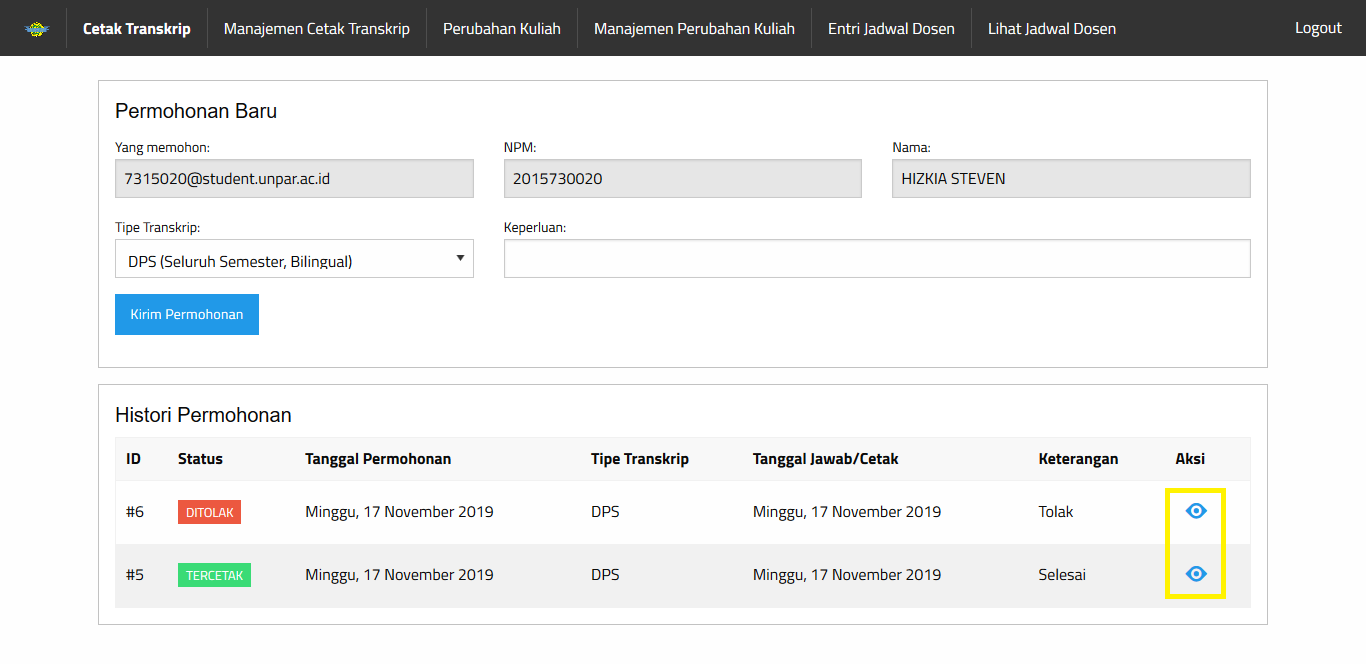
\includegraphics[scale=0.4, frame]{kriteria-sukses-2-4-4-link-purpose-in-context}  
    \caption[Pelanggaran Kriteria Sukses 2.4.4 pada Halaman Cetak Transkrip]{Pelanggaran Kriteria Sukses 2.4.4 pada Halaman Cetak Transkrip}
    \label{fig:2.4.4_link_purpose_in_context}  
\end{figure} 

\paragraph{Kriteria Sukses 2.4.5 \textit{Multiple Ways}}
\label{par:kepatuhan_bluetape_kriteria_sukses_2.4.5}
(Tidak Sukses)\\

Kriteria ini tidak sukses dipatuhi karena pada halaman web BlueTape hanya tersedia satu cara untuk menemukan suatu halaman web dalam sekumpulan halaman web yang tersedia, yaitu melalui menu navigasi. Tampilan pada halaman web dapat dilihat pada Gambar \ref{fig:2.4.5_multiple_ways}.

\begin{figure}[H]
    \centering  
    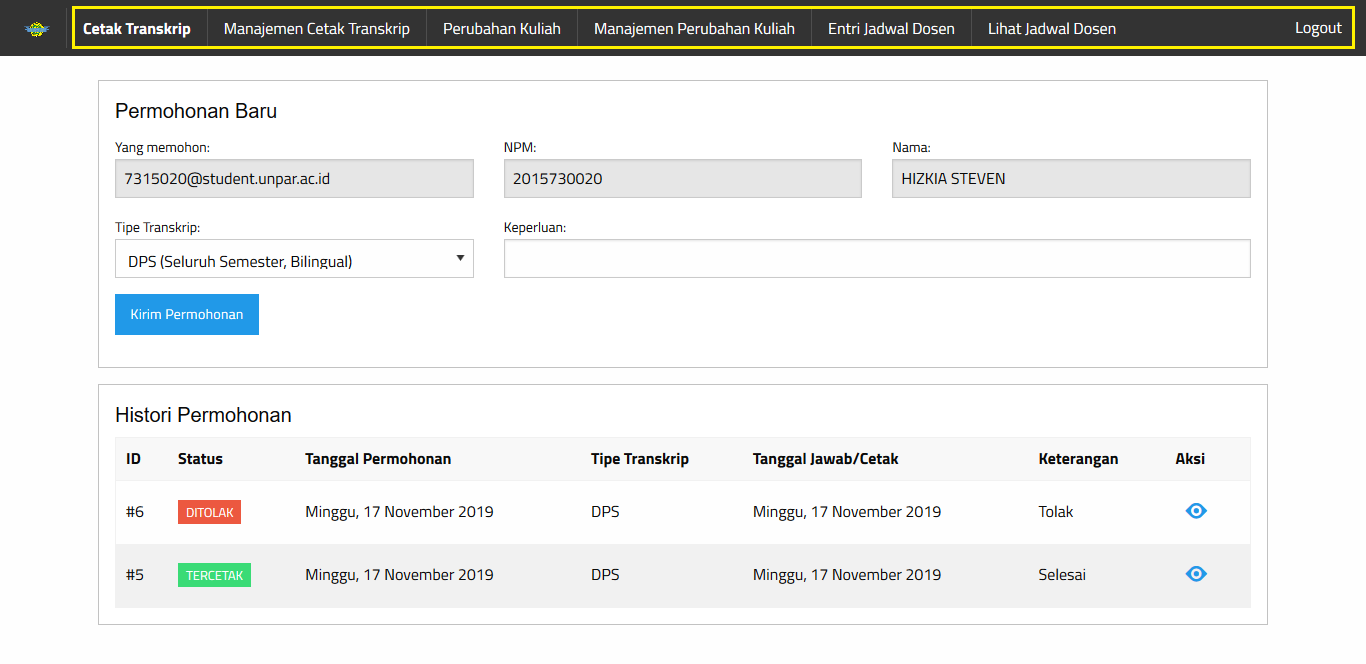
\includegraphics[scale=0.4, frame]{kriteria-sukses-2-4-5-multiple-ways}  
    \caption[Pelanggaran Kriteria Sukses 2.4.5 pada Halaman Cetak Transkrip]{Pelanggaran Kriteria Sukses 2.4.5 pada Halaman Cetak Transkrip}
    \label{fig:2.4.5_multiple_ways}  
\end{figure}

\paragraph{Kriteria Sukses 2.4.6 \textit{Headings and Labels}}
\label{par:kepatuhan_bluetape_kriteria_sukses_2.4.6}
(Tidak Sukses)\\

Kriteria ini tidak sukses dipatuhi karena pada halaman entri jadwal dosen, setiap elemen \textit{input} tidak memiliki label yang menjelaskan tujuan dari elemen tersebut. Contoh kesalahan dapat dilihat pada \textit{Listing} \ref{lst:2.4.6_label_masukan_entri_jadwal_dosen}. Tautan untuk halaman yang bermasalah dapat dilihat di \url{https://bluetape.azurewebsites.net/EntriJadwalDosen}.

\begin{lstlisting}[frame=single, label={lst:2.4.6_label_masukan_entri_jadwal_dosen}, language=HTML, caption=Pelanggaran Kriteria Sukses 2.4.6 pada Halaman Entri Jadwal Dosen]
    <input type="hidden" name="csrf_token" value="3c159eae7bc953dd591b679c080ed066"/>
    Hari
    <select name="hari">
\end{lstlisting}

\paragraph{Kriteria Sukses 2.4.7 \textit{Focus Visible}}
\label{par:kepatuhan_bluetape_kriteria_sukses_2.4.7}
(Tidak Sukses)\\

Kriteria ini tidak sukses dipatuhi karena setiap halaman web BlueTape memiliki komponen tombol dengan warna latar belakang yang sama dengan warna indikator fokus dari \textit{keyboard}. Tampilan pada halaman web dapat dilihat pada Gambar \ref{fig:2.4.7_focus_visible}. Contoh tautan untuk halaman yang bermasalah dapat dilihat di \url{https://bluetape.azurewebsites.net/TranskripRequest}. 

\begin{figure}[H]
    \centering  
    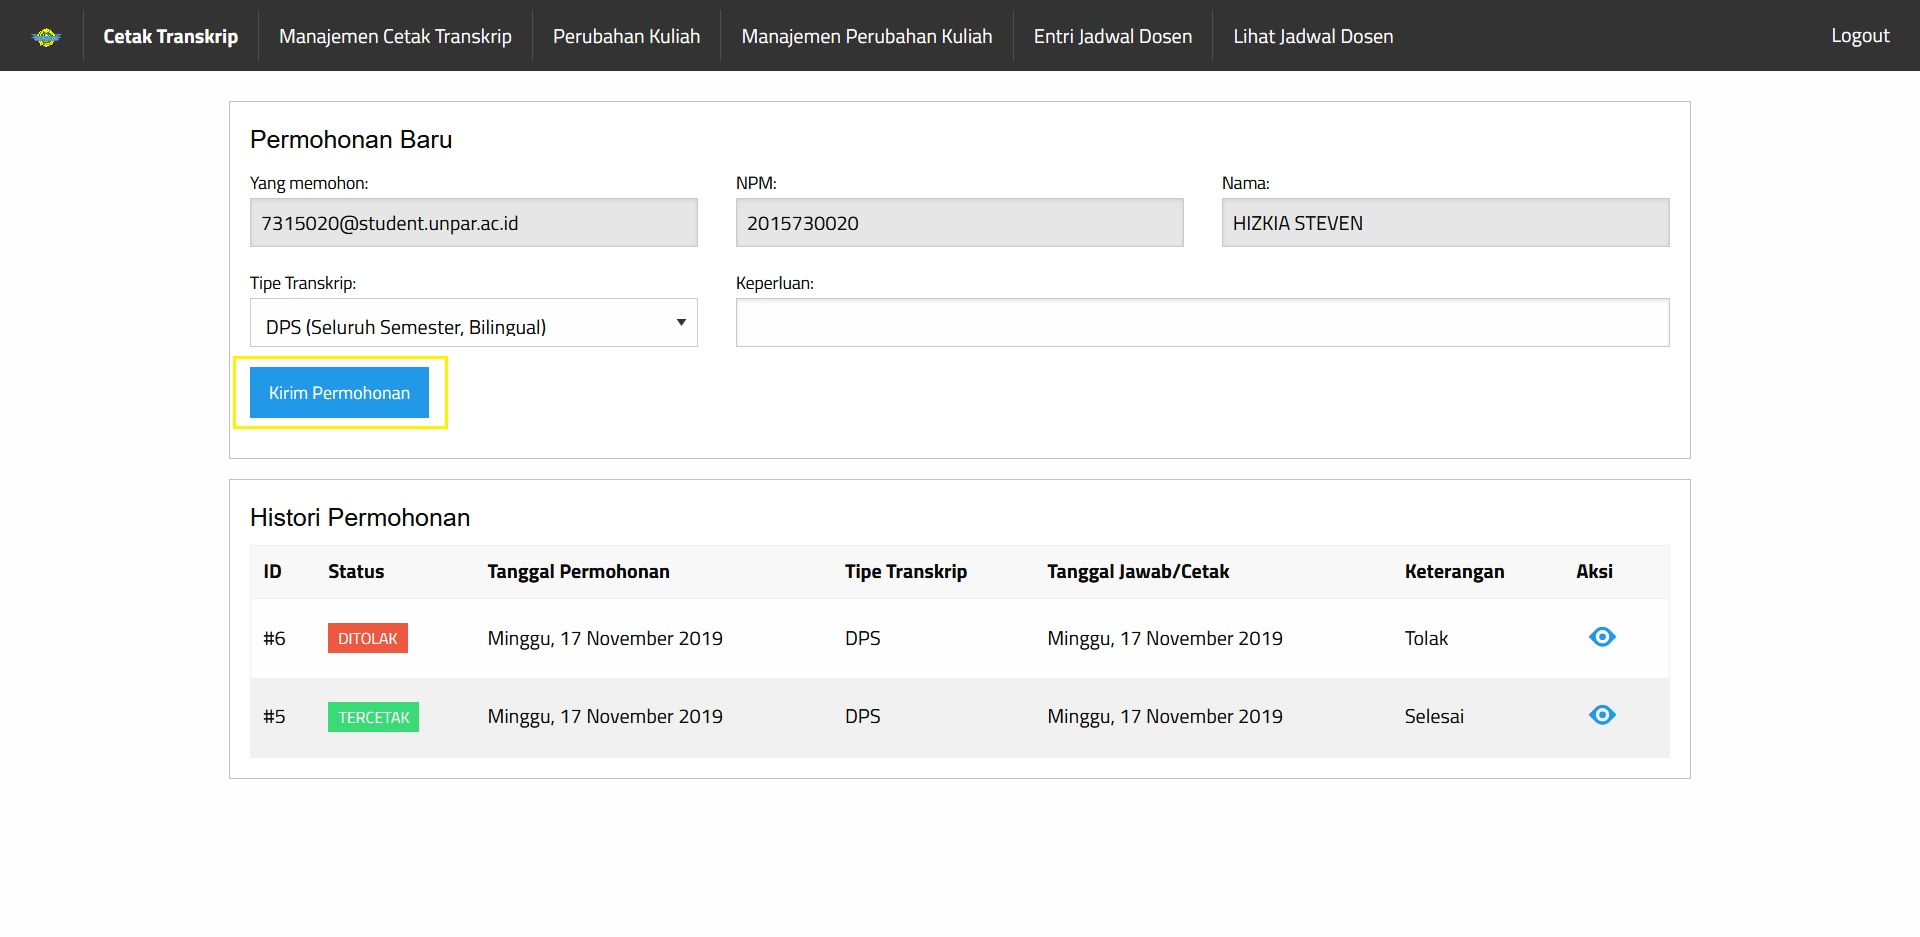
\includegraphics[scale=0.4, frame]{kriteria-sukses-2-4-7-focus-visible}  
    \caption[Pelanggaran Kriteria Sukses 2.4.7 pada Halaman Cetak Transkrip]{Pelanggaran Kriteria Sukses 2.4.7 pada Halaman Cetak Transkrip}
    \label{fig:2.4.7_focus_visible}  
\end{figure}

\paragraph{Kriteria Sukses 2.4.8 \textit{Location}}
\label{par:kepatuhan_bluetape_kriteria_sukses_2.4.8}
(Sukses)\\

Kriteria ini sukses dipatuhi karena pada menu navigasi terdapat indikator yang menunjukkan halaman yang sedang dipilih oleh pengguna, indikator ini berupa penebalan ukuran tulisan.

\paragraph{Kriteria Sukses 2.4.9 \textit{Link Purpose (Link Only)}}
\label{par:kepatuhan_bluetape_kriteria_sukses_2.4.9}
(Tidak Sukses)\\

Kriteria ini tidak sukses dipatuhi karena pada halaman cetak transkrip, manajemen cetak transkrip, perubahan kuliah, dan manajemen perubahan kuliah terdapat tautan yang berisi konten bukan teks dan tidak terdapat teks yang dapat menjelaskan tujuan tautan tersebut. Kesalahan dapat dilihat pada \textit{Listing} \ref{lst:2.4.9_tautan_tanpa_keterangan}. Tampilan pada halaman web dapat dilihat pada Gambar \ref{fig:2.4.9_link_purpose_link_only}. Contoh tautan untuk halaman yang bermasalah dapat dilihat di \url{https://bluetape.azurewebsites.net/TranskripRequest}.

\begin{lstlisting}[frame=single, label={lst:2.4.9_tautan_tanpa_keterangan}, language=HTML, caption=Pelanggaran Kriteria Sukses 2.4.9 pada Halaman Cetak Transkrip]
        </div>
        <a data-open="detail6">
            <i class="fi-eye"></i>
        </a>
    </td>
\end{lstlisting}

\begin{figure}[H]
    \centering  
    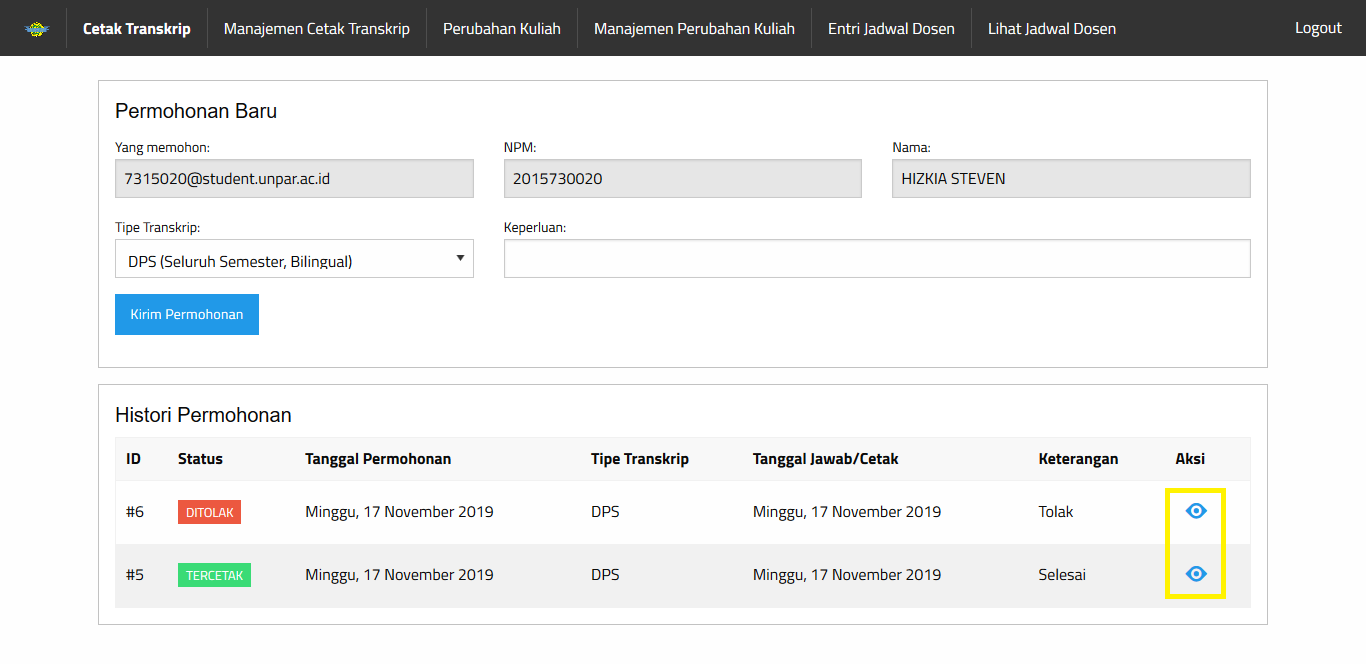
\includegraphics[scale=0.4, frame]{kriteria-sukses-2-4-9-link-purpose-link-only}  
    \caption[Pelanggaran Kriteria Sukses 2.4.9 pada Halaman Cetak Transkrip]{Pelanggaran Kriteria Sukses 2.4.9 pada Halaman Cetak Transkrip}
    \label{fig:2.4.9_link_purpose_link_only}  
\end{figure} 

\paragraph{Kriteria Sukses 2.4.10 \textit{Section Headings}}
\label{par:kepatuhan_bluetape_kriteria_sukses_2.4.10}
(Tidak Sukses)\\

Kriteria ini tidak sukses dipatuhi karena terdapat penggunaan \textit{tag heading} yang tidak tepat secara struktur pada halaman cetak transkrip, manajemen cetak transkrip, perubahan kuliah, manajemen perubahan kuliah, dan entri jadwal dosen. Contoh kesalahan dapat dilihat pada \textit{Listing} \ref{lst:1.3.1_heading_tidak_tepat} yang menampilkan kesalahan penggunaan \textit{tag heading} pada halaman cetak transkrip. Contoh tautan untuk halaman yang bermasalah dapat dilihat di \url{https://bluetape.azurewebsites.net/TranskripRequest}.

\begin{lstlisting}[frame=single, label={lst:2.4.10_heading_tidak_tepat}, language=HTML, caption=Pelanggaran Kriteria Sukses 2.4.10 pada Halaman Cetak Transkrip]
    <div class="callout">
        <h5>Permohonan Baru</h5>
        <form method="POST" action="/TranskripRequest/add">
\end{lstlisting}

\subsubsection{\textit{Input Modalities}}
\label{subsubsec:kepatuhan_bluetape_input_modalities}
Pada subbab ini dibahas alasan mengapa poin kriteria sukses pada kategori \textit{input modalities} dinilai sukses atau tidak sukses.

\paragraph{Kriteria Sukses 2.5.1 \textit{Pointer Gestures}}
\label{par:kepatuhan_bluetape_kriteria_sukses_2.5.1}
(Sukses)\\

Kriteria ini sukses dipatuhi karena pada halaman web BlueTape tidak terdapat fungsionalitas yang harus dijalankan dengan menggunakan \textit{multipoint} atau gestur berbasis \textit{path}.

\paragraph{Kriteria Sukses 2.5.2 \textit{Pointer Cancellation}}
\label{par:kepatuhan_bluetape_kriteria_sukses_2.5.2}
(Sukses)\\

Kriteria ini sukses dipatuhi karena setiap fungsionalitas yang dapat dioperasikan dengan kursor tunggal tidak memiliki \textit{down-event}.

\paragraph{Kriteria Sukses 2.5.3 \textit{Label in Name}}
\label{par:kepatuhan_bluetape_kriteria_sukses_2.5.3}
(Tidak Sukses)\\

Kriteria ini tidak sukses dipatuhi karena pada halaman manajemen cetak transkrip dan entri jadwal dosen, elemen \textit{input} yang memiliki label yang menyertakan teks tidak memiliki teks nama yang dapat diidentifikasi oleh teknologi alat bantu. Contoh kesalahan dapat dilihat pada \textit{Listing} \ref{lst:2.5.3_label_dan_nama_pada_komponen_masukan}. Contoh tautan untuk halaman yang bermasalah dapat dilihat di \url{https://bluetape.azurewebsites.net/TranskripManage}.

\begin{lstlisting}[frame=single, label={lst:2.5.3_label_dan_nama_pada_komponen_masukan}, language=HTML, caption=Pelanggaran Kriteria Sukses 2.5.3 pada Halaman Manajemen Cetak Transkrip]
    <div class="input-group">
        <span class="input-group-label">Cari NPM:</span>
        <input name="npm" class="input-group-field" type="text" placeholder="2013730013" maxlength="10" minlength="10"<?= $npmQuery === NULL ? '' : " value='$npmQuery'" ?>/>
        <div class="input-group-button">
            <input class="button" type="submit" value="Cari"/>
        </div>
    </div>
\end{lstlisting}

\paragraph{Kriteria Sukses 2.5.4 \textit{Motion Actuation}}
\label{par:kepatuhan_bluetape_kriteria_sukses_2.5.4}
(Sukses)\\

Kriteria ini sukses dipatuhi karena tidak terdapat fungsionalitas yang dapat dioperasikan oleh gerakan perangkat atau gerakan pengguna.

\paragraph{Kriteria Sukses 2.5.5 \textit{Target Size}}
\label{par:kepatuhan_bluetape_kriteria_sukses_2.5.5}
(Tidak Sukses)\\

Kriteria ini tidak sukses dipatuhi karena terdapat banyak elemen yang dapat menerima \textit{input} kursor dan ukurannya diatur oleh penulis namun memiliki ukuran kurang dari 44 $\times$ 44 piksel \textit{CSS}. Contoh tampilan pada halaman web dapat dilihat pada Gambar \ref{fig:2.5.5_target_size}. Contoh tautan untuk halaman yang bermasalah dapat dilihat di \url{https://bluetape.azurewebsites.net/TranskripRequest}.

\begin{figure}[H]
    \centering  
    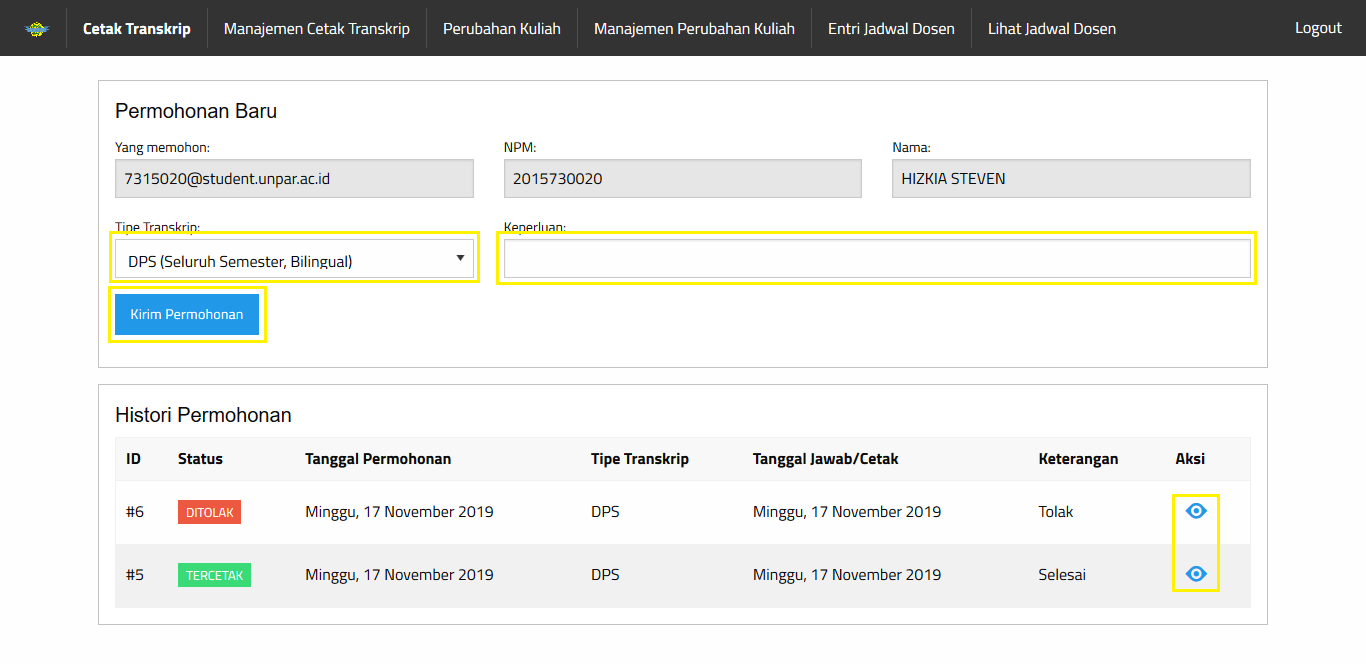
\includegraphics[scale=0.4, frame]{kriteria-sukses-2-5-5-target-size}  
    \caption[Pelanggaran Kriteria Sukses 2.5.5 pada Halaman Cetak Transkrip]{Pelanggaran Kriteria Sukses 2.5.5 pada Halaman Cetak Transkrip}
    \label{fig:2.5.5_target_size}  
\end{figure} 

\paragraph{Kriteria Sukses 2.5.6 \textit{Concurrent Input Mechanisms}}
\label{par:kepatuhan_bluetape_kriteria_sukses_2.5.6}
(Sukses)\\

Kriteria ini sukses dipatuhi karena konten web BlueTape tidak membatasi penggunaan mode \textit{input} yang tersedia pada platform.

\subsection{\textit{Understandable}}
\label{subsec:kepatuhan_bluetape_understandable}
Pada subbab ini dibahas kriteria-kriteria sukses yang termasuk ke dalam kategori \textit{understandable}. Hasil sukses atau tidaknya aplikasi BlueTape terhadap poin-poin kriteria sukses dalam kategori ini ditampilkan pada Tabel \ref{tab:kepatuhan_bluetape_understandable}.

\begin{table}[H]
    \centering 
    \caption{Kepatuhan BlueTape terhadap prinsip \textit{Understandable}}
    \label{tab:kepatuhan_bluetape_understandable}
    \begin{tabular}{|c|c|c|}
        \toprule
        Kriteria Sukses & Hasil (sukses/tidak) & Tingkat Kepatuhan \\

        \midrule
        \rowcolor{darkred} 3.1.1 & Tidak Sukses & A \\
        \rowcolor{brightred} 3.1.2 & Tidak Sukses & AA \\
        \rowcolor{pink} 3.1.3 & Tidak Sukses & AAA \\
        \rowcolor{pink} 3.1.4 & Tidak Sukses & AAA \\
        3.1.5 & Sukses & AAA \\
        3.1.6 & Sukses & AAA \\
        3.2.1 & Sukses & A \\
        3.2.2 & Sukses & A \\
        3.2.3 & Sukses & AA \\
        \rowcolor{brightred} 3.2.4 & Tidak Sukses & AA \\
        3.2.5 & Sukses & AAA \\
        3.3.1 & Sukses & A \\
        \rowcolor{darkred} 3.3.2 & Tidak Sukses & A \\
        3.3.3 & Sukses & AA \\
        3.3.4 & Sukses & AA \\
        \rowcolor{pink} 3.3.5 & Tidak Sukses & AAA \\
        3.3.6 & Sukses & AAA \\

        \bottomrule
        \multicolumn{2}{|c|}{Tingkat kepatuhan tertinggi yang dicapai} & - \\
        \bottomrule

    \end{tabular}
\end{table}

\subsubsection{\textit{Readable}}
\label{subsubsec:kepatuhan_bluetape_readable}
Pada subbab ini dibahas alasan mengapa poin kriteria sukses pada kategori \textit{readable} dinilai sukses atau tidak sukses.

\paragraph{Kriteria Sukses 3.1.1 \textit{Language of Page}}
\label{par:kepatuhan_bluetape_kriteria_sukses_3.1.1}
(Tidak Sukses)\\

Kriteria ini tidak sukses dipatuhi karena bahasa manusia \textit{default} yang digunakan pada halaman web BlueTape tidak sesuai dengan konten yang disajikan pada halaman tersebut. Bahasa manusia \textit{default} yang digunakan pada halaman web BlueTape adalah bahasa Inggris sementara konten disajikan dalam bahasa Indonesia. Contoh kesalahan dapat dilihat pada \textit{Listing} \ref{lst:3.1.1_bahasa_halaman}. Contoh tautan untuk halaman yang bermasalah dapat dilihat di \url{https://bluetape.azurewebsites.net/TranskripRequest}.

\begin{lstlisting}[frame=single, label={lst:3.1.1_bahasa_halaman}, language=HTML, caption=Pelanggaran Kriteria Sukses 3.1.1 pada Halaman Cetak Transkrip]
    // Setelan bahasa diatur menjadi bahasa Inggris
    <!DOCTYPE html>
        <html class="no-js" lang="en">
    <head>

    // Konten disajikan dalam bahasa Indonesia
    <div class="large-4 column">
        <label>Yang memohon:
            <input type="email" name="requestByEmail" value="7315020@student.unpar.ac.id" readonly="readonly"/>
        </label>
    </div>
    <div class="large-4 column">
        <label>NPM:
            <input type="text" value="2015730020" readonly="readonly"/>
        </label>
    </div>
    <div class="large-4 column">
        <label>Nama:
            <input type="text" name="requestByName" value="HIZKIA STEVEN" readonly="readonly"/>
        </label>
    </div>
\end{lstlisting}

\paragraph{Kriteria Sukses 3.1.2 \textit{Language of Parts}}
\label{par:kepatuhan_bluetape_kriteria_sukses_3.1.2}
(Tidak Sukses)\\

Kriteria ini tidak sukses dipatuhi karena pada halaman web BlueTape terdapat konten teks dalam bahasa Inggris namun konten tersebut tidak memiliki atribut \textit{lang}. Konten yang dimaksud adalah:

\begin{itemize}
    \item Pada bagian menu navigasi terdapat elemen dengan teks "Logout". Letak kesalahan dapat dilihat pada \textit{Listing} \ref{lst:3.1.2_bahasa_pada_navigasi}. Contoh tampilan pada halaman web dapat dilihat pada Gambar \ref{fig:3.1.2_language_of_parts_1}. 
    \begin{lstlisting}[frame=single, label={lst:3.1.2_bahasa_pada_navigasi}, language=HTML, caption=Pelanggaran Kriteria Sukses 3.1.2 pada Menu Navigasi]
        <ul class="menu">
            <li><a href="/auth/logout">Logout</a></li>
        </ul>
    \end{lstlisting}
    
    \begin{figure}[H]
        \centering  
        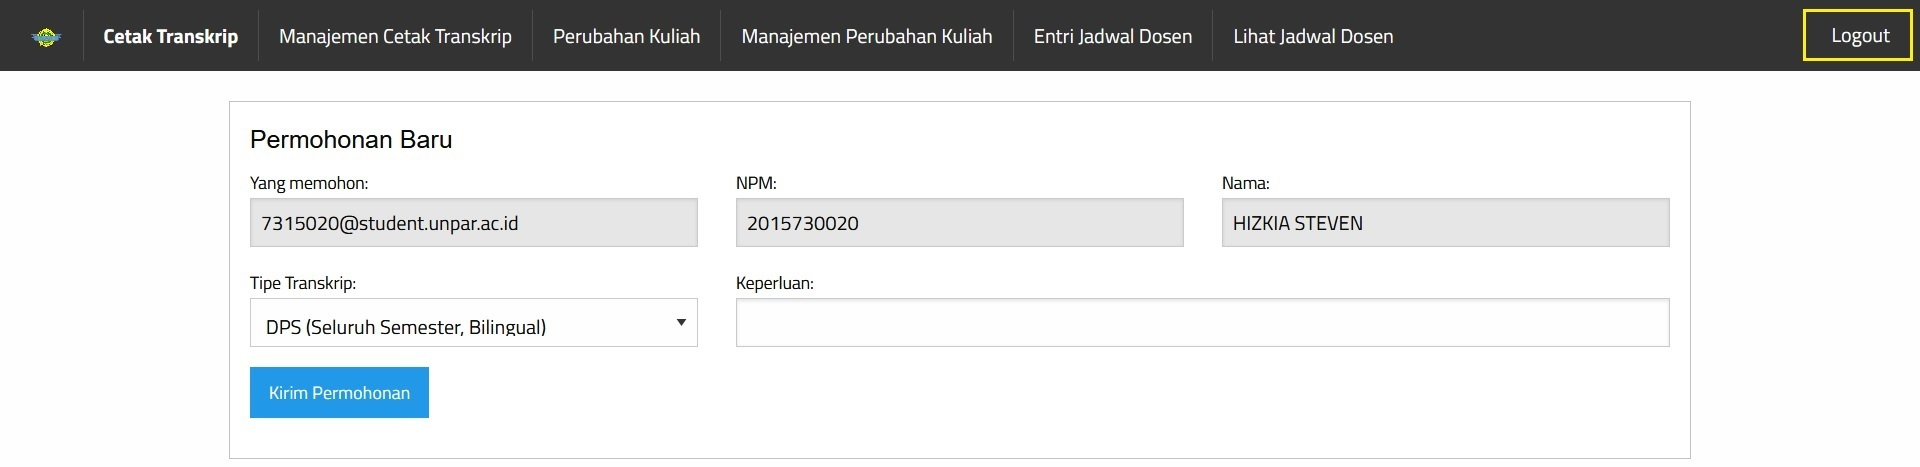
\includegraphics[scale=0.4, frame]{kriteria-sukses-3-1-2-language-of-parts-1}  
        \caption[Pelanggaran Kriteria Sukses 3.1.2 pada Menu Navigasi]{Pelanggaran Kriteria Sukses 3.1.2 pada Menu Navigasi}
        \label{fig:3.1.2_language_of_parts_1}  
    \end{figure}

    \item Pada halaman entri jadwal dosen terdapat tombol dengan teks "Delete All". Letak kesalahan dapat dilihat pada \textit{Listing} \ref{lst:3.1.2_bahasa_pada_halaman_entri_jadwal_dosen_1}. Contoh tampilan pada halaman web dapat dilihat pada Gambar \ref{fig:3.1.2_language_of_parts_2}. Tautan untuk halaman yang bermasalah dapat dilihat di \url{https://bluetape.azurewebsites.net/EntriJadwalDosen}.
    \begin{lstlisting}[frame=single, label={lst:3.1.2_bahasa_pada_halaman_entri_jadwal_dosen_1}, language=HTML, caption=Pelanggaran Kriteria Sukses 3.1.2 pada Halaman Entri Jadwal Dosen]
        <a href="/EntriJadwalDosen/deleteAll/export/" class="alert button" onClick="return konfirmasi();">
            Delete All
        </a>
    \end{lstlisting}
    
    \begin{figure}[H]
        \centering  
        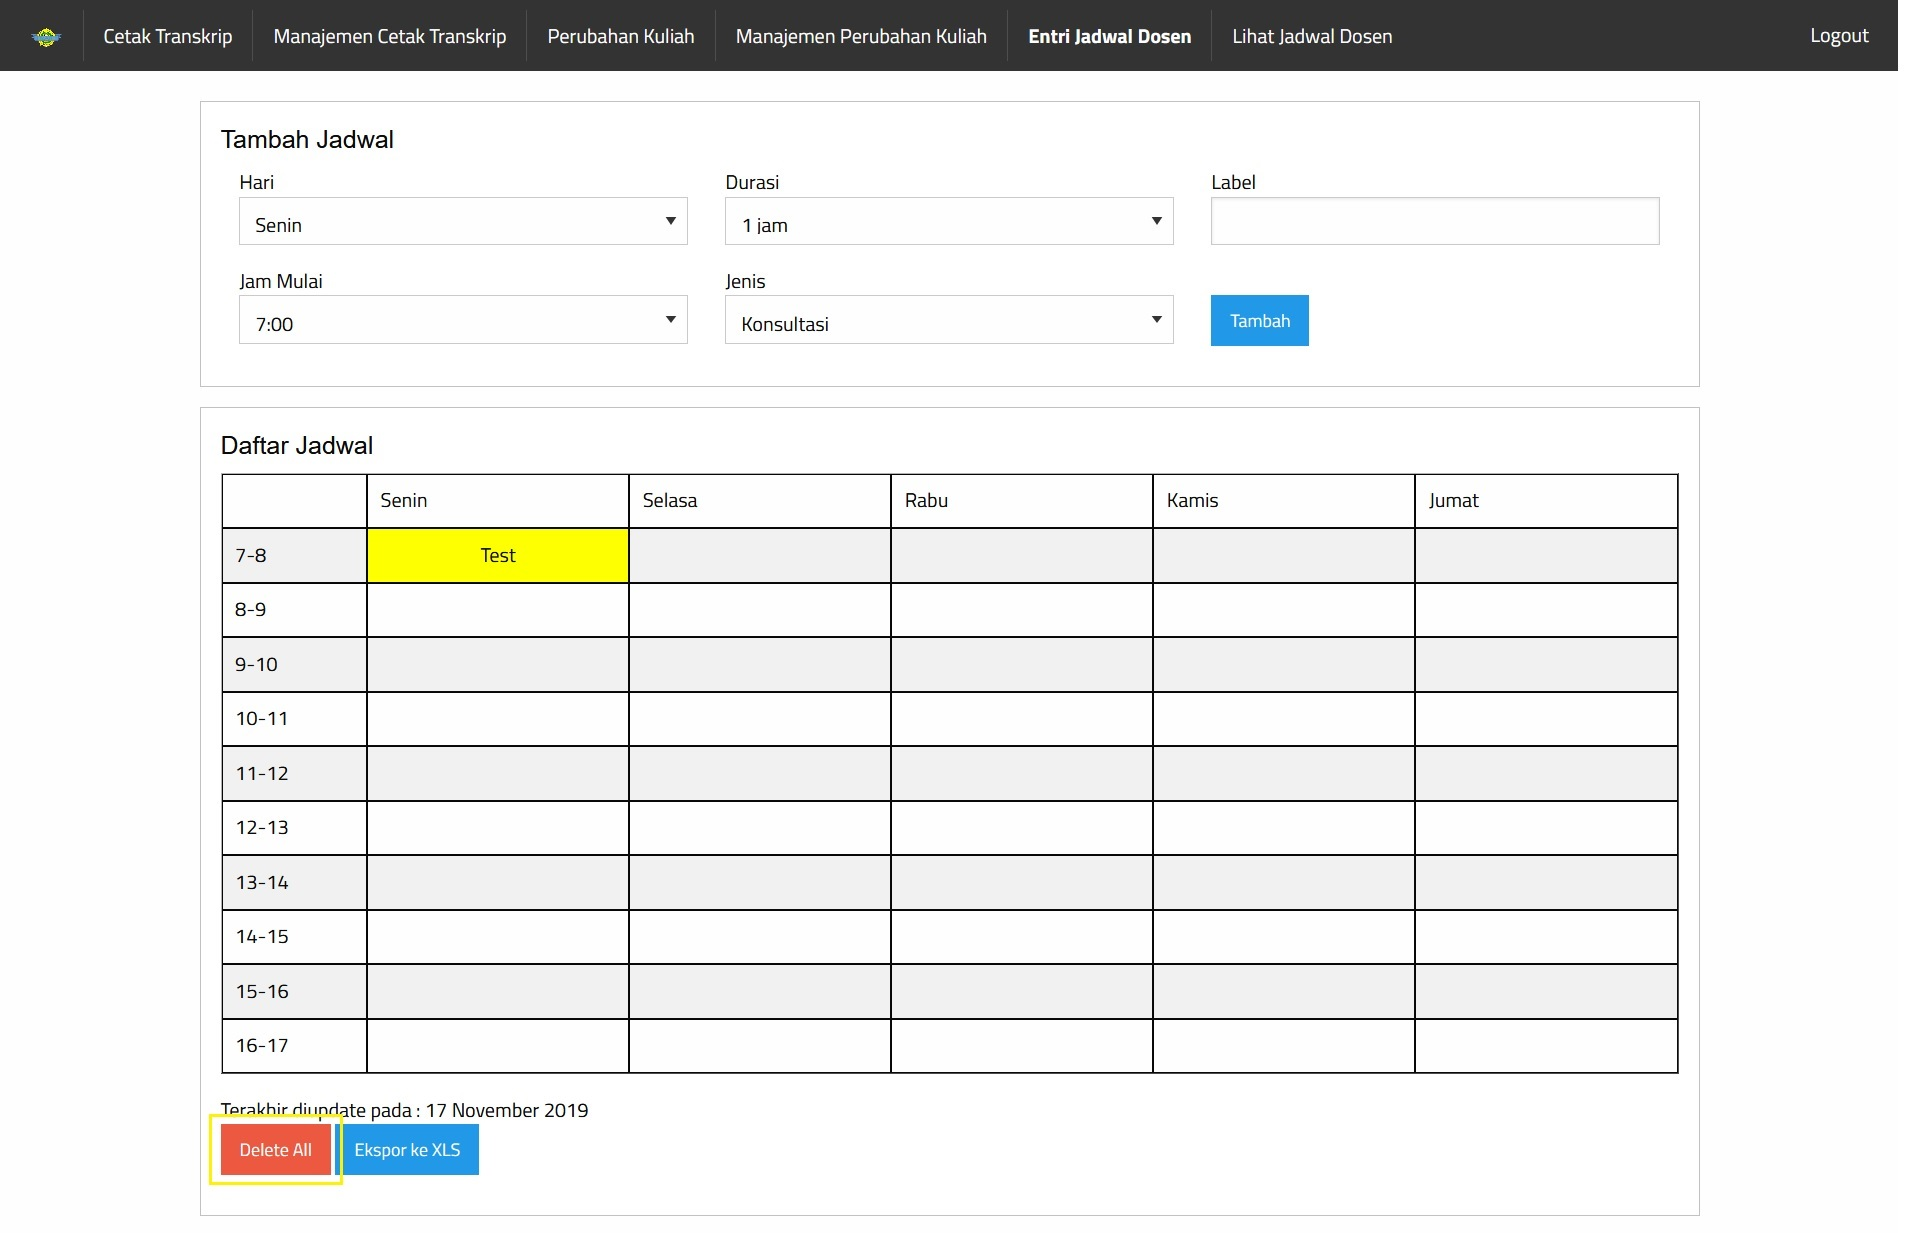
\includegraphics[scale=0.4, frame]{kriteria-sukses-3-1-2-language-of-parts-2}  
        \caption[Pelanggaran Kriteria Sukses 3.1.2 pada Halaman Entri Jadwal Dosen]{Pelanggaran Kriteria Sukses 3.1.2 pada Halaman Entri Jadwal Dosen}
        \label{fig:3.1.2_language_of_parts_2}  
    \end{figure}
    
    \item Pada halaman entri jadwal dosen bagian "Edit Jadwal" terdapat tombol dengan teks "Save" dan tombol dengan teks "Delete". Letak kesalahan dapat dilihat pada \textit{Listing} \ref{lst:3.1.2_bahasa_pada_halaman_entri_jadwal_dosen_2}. Contoh tampilan pada halaman web dapat dilihat pada Gambar \ref{fig:3.1.2_language_of_parts_3}. Tautan untuk halaman yang bermasalah dapat dilihat di \url{https://bluetape.azurewebsites.net/EntriJadwalDosen}.
    \begin{lstlisting}[frame=single, label={lst:3.1.2_bahasa_pada_halaman_entri_jadwal_dosen_2}, language=HTML, caption=Pelanggaran Kriteria Sukses 3.1.2 pada Kotak Dialog di Halaman Entri Jadwal Dosen]
        // Tombol "Save"
        <div class="large-2 column">
            <input type="submit" name="submitId8" class="button" value="Save">
            </form>
        </div>

        // Tombol "Delete"
        <form name="formDelete8" method="POST" action="/EntriJadwalDosen/delete/8">    
            <input type="hidden" name="csrf_token" value="3c159eae7bc953dd591b679c080ed066"/>
            <input id="deletebtn8" name="8" type="submit" class="alert button" value="Delete">
        </form><div>
    \end{lstlisting}
    
    \begin{figure}[H]
        \centering  
        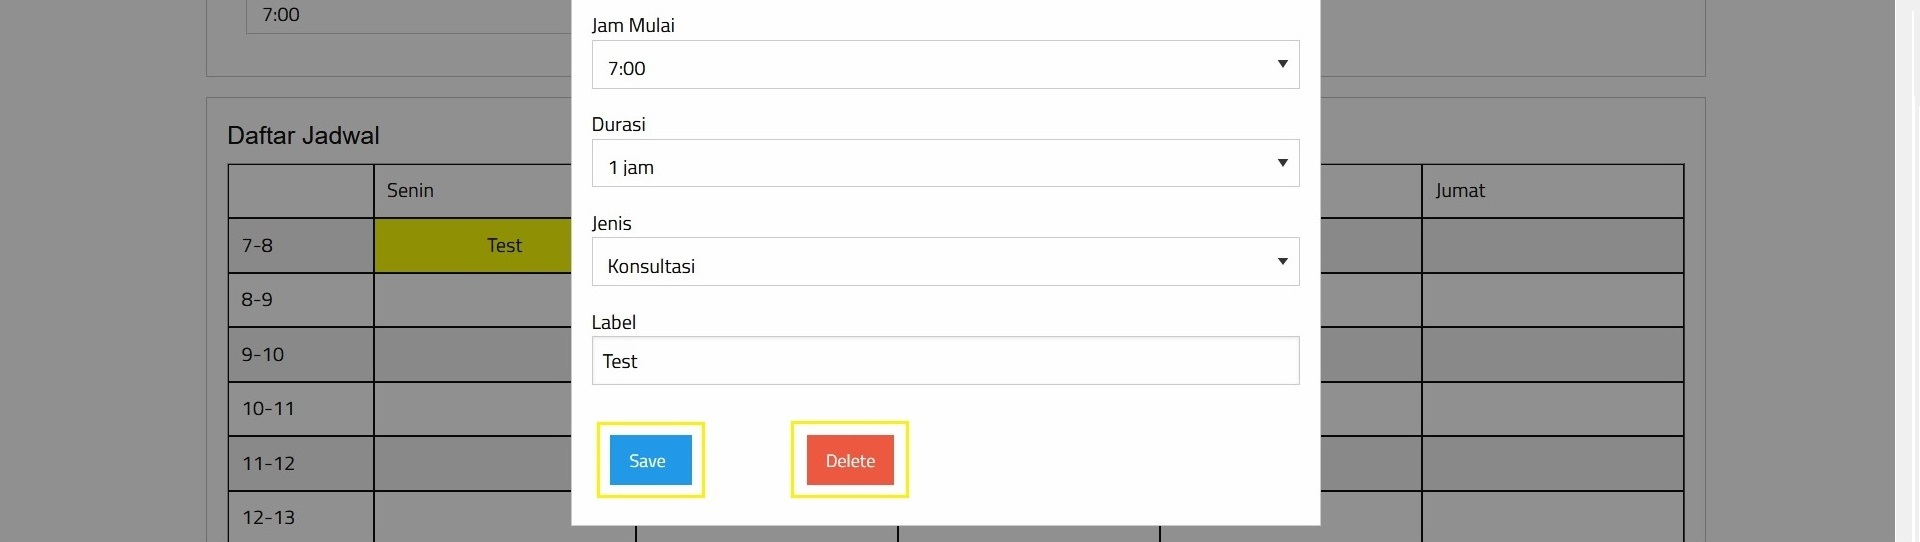
\includegraphics[scale=0.4, frame]{kriteria-sukses-3-1-2-language-of-parts-3}  
        \caption[Pelanggaran Kriteria Sukses 3.1.2 pada Kotak Dialog di Halaman Entri Jadwal Dosen]{Pelanggaran Kriteria Sukses pada Kotak Dialog di Halaman Entri Jadwal Dosen}
        \label{fig:3.1.2_language_of_parts_3}  
    \end{figure}
\end{itemize}

\paragraph{Kriteria Sukses 3.1.3 \textit{Unusual Words}}
\label{par:kepatuhan_bluetape_kriteria_sukses_3.1.3}
(Tidak Sukses)\\

Kriteria ini tidak sukses dipatuhi karena terdapat kata-kata yang digunakan dengan cara yang tidak lazim atau terbatas namun tidak tersedia mekanisme untuk mengidentifikasi definisi spesifik dari kata-kata tersebut. Kata-kata yang dimaksud adalah:

\begin{itemize}
    \item Pada halaman perubahan kuliah, tombol dengan teks "Tambah Pertemuan Ekstra". Letak kesalahan dapat dilihat pada \textit{Listing} \ref{lst:3.1.3_kata_pada_halaman_perubahan_kuliah}. Contoh tampilan pada halaman web dapat dilihat pada Gambar \ref{fig:3.1.3_unusual_words_1}. Tautan untuk halaman yang bermasalah dapat dilihat di \url{https://bluetape.azurewebsites.net/PerubahanKuliahRequest}.
    \begin{lstlisting}[frame=single, label={lst:3.1.3_kata_pada_halaman_perubahan_kuliah}, language=HTML, caption=Pelanggaran Kriteria Sukses 3.1.3 pada Halaman Perubahan Kuliah]
            <a href="#" id="addToButton" class="button secondary">
                Tambah Pertemuan Ekstra
            </a>
    \end{lstlisting}
    
    \begin{figure}[H]
        \centering  
        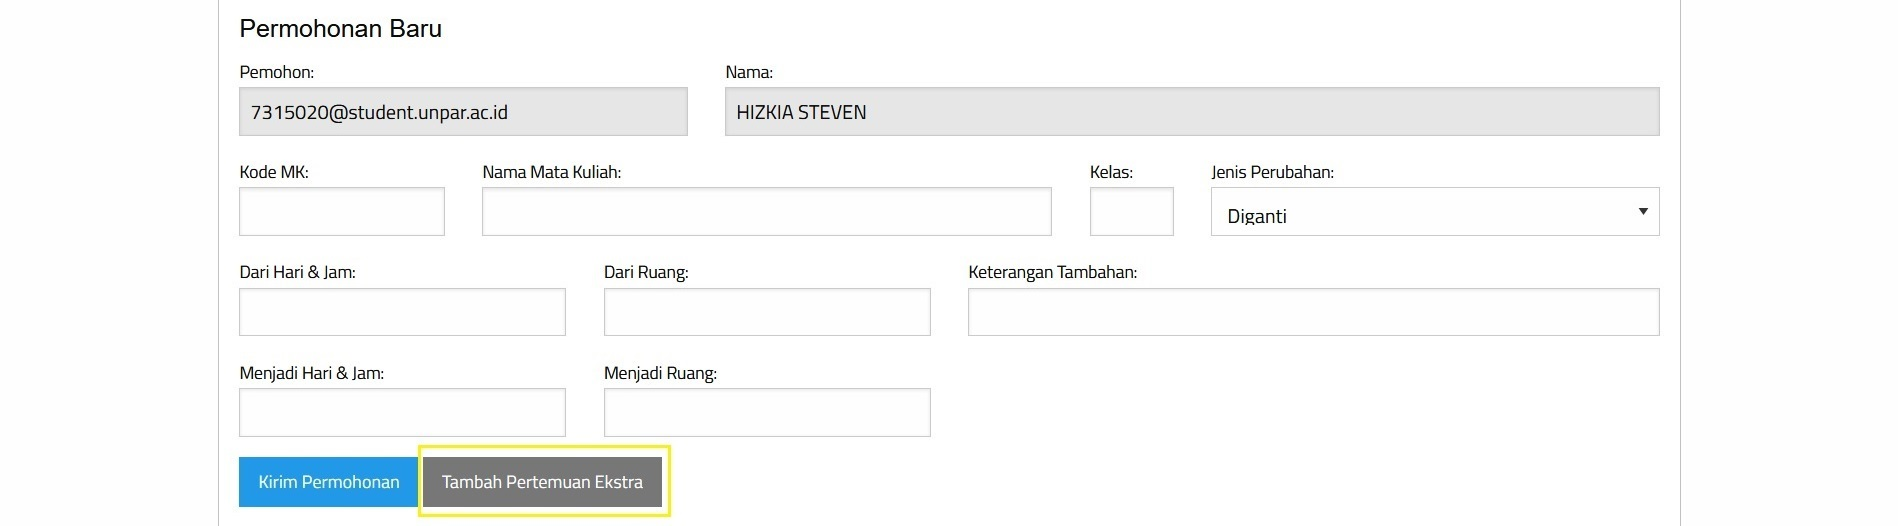
\includegraphics[scale=0.4, frame]{kriteria-sukses-3-1-3-unusual-words-1}  
        \caption[Pelanggaran Kriteria Sukses 3.1.3 pada Halaman Perubahan Kuliah]{Pelanggaran Kriteria Sukses 3.1.3 pada Halaman Perubahan Kuliah}
        \label{fig:3.1.3_unusual_words_1}  
    \end{figure}
    
    \item Pada halaman entri jadwal dosen, tombol dengan teks "Ekspor ke XLS". Letak kesalahan dapat dilihat pada \textit{Listing} \ref{lst:3.1.3_kata_pada_halaman_entri_jadwal_dosen}. Contoh tampilan pada halaman web dapat dilihat pada Gambar \ref{fig:3.1.3_unusual_words_2}. Tautan untuk halaman yang bermasalah dapat dilihat di \url{https://bluetape.azurewebsites.net/EntriJadwalDosen}.
    \begin{lstlisting}[frame=single, label={lst:3.1.3_kata_pada_halaman_entri_jadwal_dosen}, language=HTML, caption=Pelanggaran Kriteria Sukses 3.1.3 pada Halaman Entri Jadwal Dosen]
        <a href="/EntriJadwalDosen/export/" class="button">
            Ekspor ke XLS
        </a>
    \end{lstlisting}
    
    \begin{figure}[H]
        \centering  
        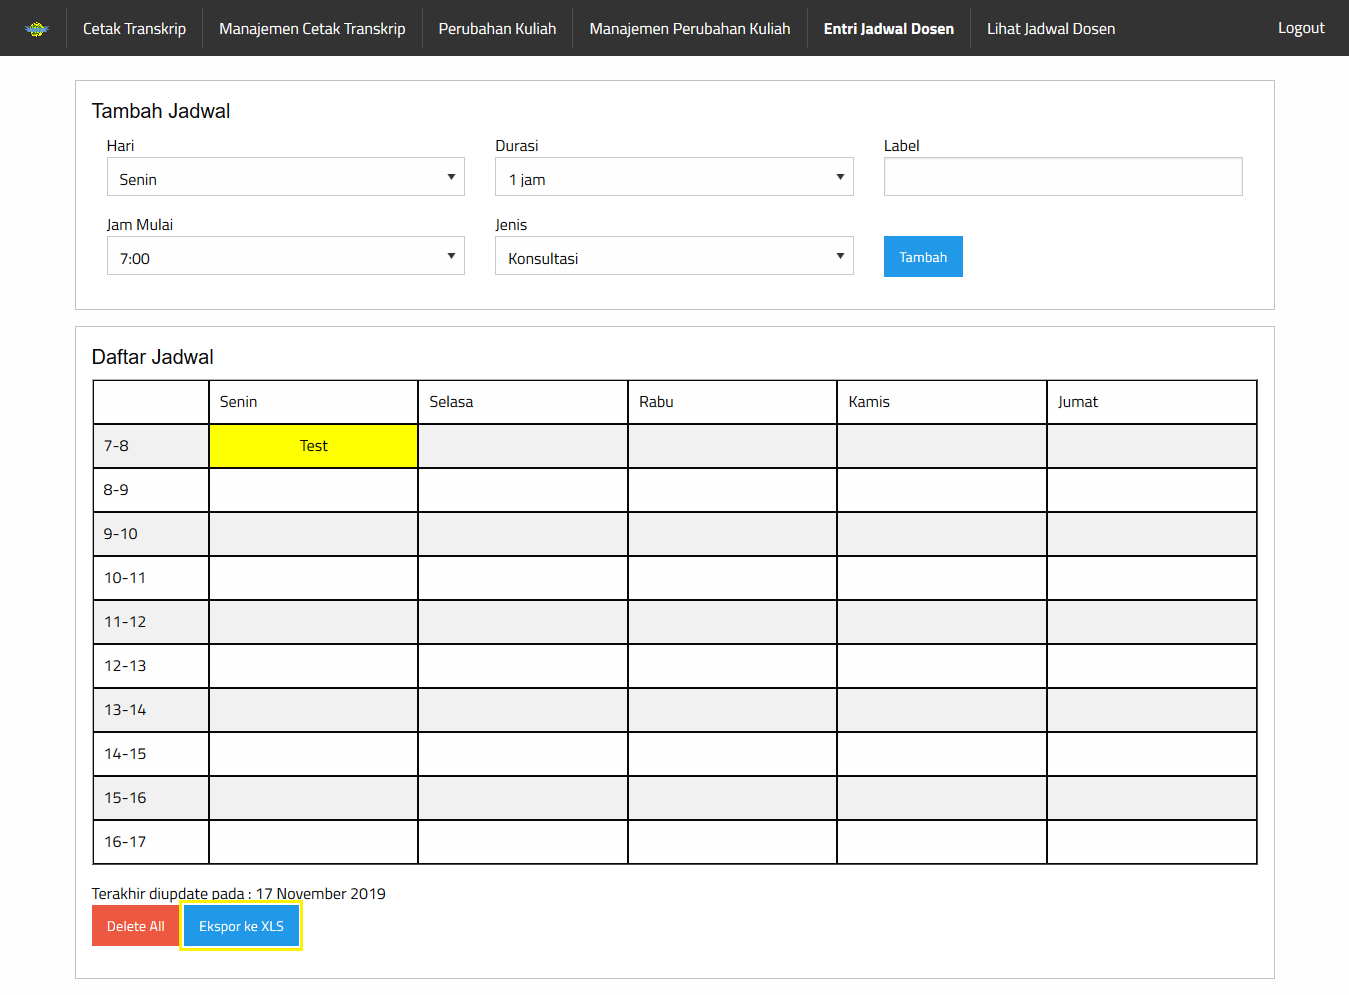
\includegraphics[scale=0.4, frame]{kriteria-sukses-3-1-3-unusual-words-2}  
        \caption[Pelanggaran Kriteria Sukses 3.1.3 pada Halaman Entri Jadwal Dosen]{Pelanggaran Kriteria Sukses 3.1.3 pada Halaman Entri Jadwal Dosen}
        \label{fig:3.1.3_unusual_words_2}  
    \end{figure}

    \item Pada halaman lihat jadwal dosen, tombol dengan teks "Ekspor ke XLS". Letak kesalahan dapat dilihat pada \textit{Listing} \ref{lst:3.1.3_kata_pada_halaman_lihat_jadwal_dosen}. Contoh tampilan pada halaman web dapat dilihat pada Gambar \ref{fig:3.1.3_unusual_words_3}. Tautan untuk halaman yang bermasalah dapat dilihat di \url{https://bluetape.azurewebsites.net/LihatJadwalDosen}.
    \begin{lstlisting}[frame=single, label={lst:3.1.3_kata_pada_halaman_lihat_jadwal_dosen}, language=HTML, caption=Pelanggaran Kriteria Sukses 3.1.3 pada Halaman Lihat Jadwal Dosen]
        <a href="/LihatJadwalDosen/export/" class="button">
            Ekspor ke XLS
        </a>
    \end{lstlisting}
    
    \begin{figure}[H]
        \centering  
        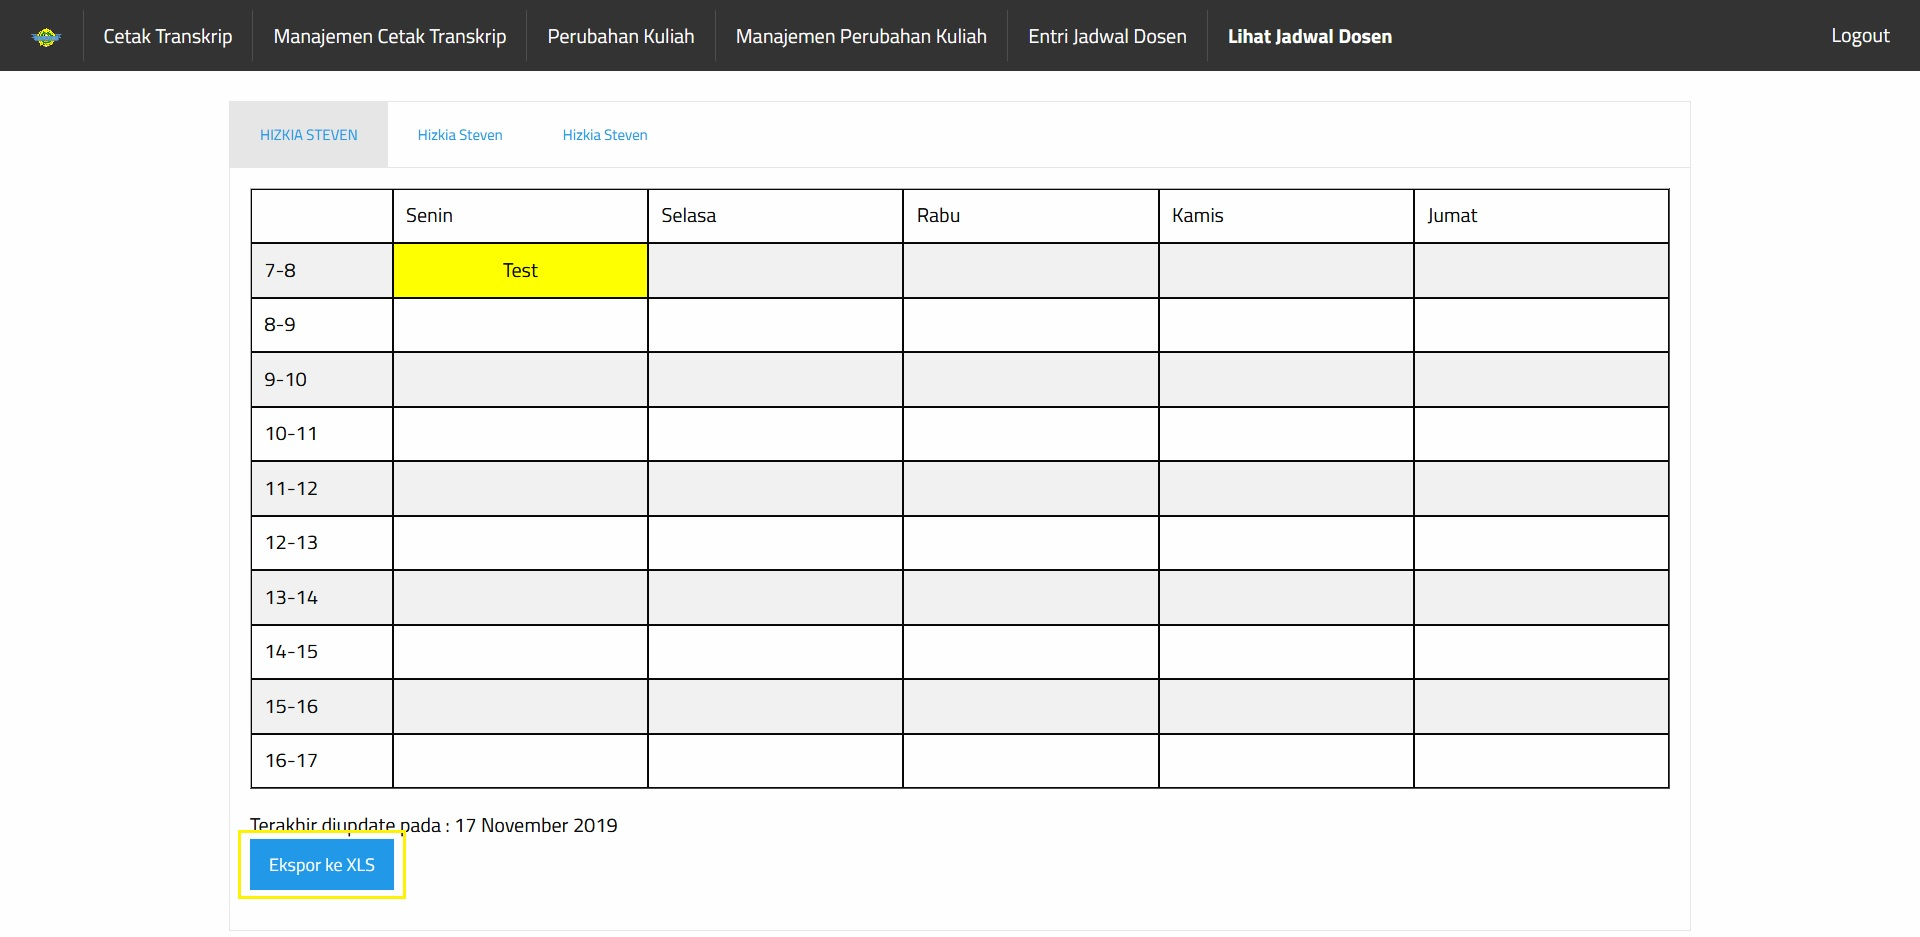
\includegraphics[scale=0.4, frame]{kriteria-sukses-3-1-3-unusual-words-3}  
        \caption[Pelanggaran Kriteria Sukses 3.1.3 pada Halaman Lihat Jadwal Dosen]{Pelanggaran Kriteria Sukses 3.1.3 pada Halaman Lihat Jadwal Dosen}
        \label{fig:3.1.3_unusual_words_3}  
    \end{figure}
    
\end{itemize}

\paragraph{Kriteria Sukses 3.1.4 \textit{Abbreviations}}
\label{par:kepatuhan_bluetape_kriteria_sukses_3.1.4}
(Tidak Sukses)\\

Kriteria ini tidak sukses dipatuhi karena tidak tersedia mekanisme untuk mengidentifikasi kepanjangan dari singkatan. Singkatan-singkatan yang terdapat pada halaman web BlueTape, antara lain:

\begin{itemize}
    \item Pada halaman cetak transkrip terdapat singkatan "NPM" dan "DPS". Letak kesalahan dapat dilihat pada \textit{Listing} \ref{lst:3.1.4_singkatan_pada_halaman_cetak_transkrip}. Contoh tampilan pada halaman web dapat dilihat pada Gambar \ref{fig:3.1.4_abbreviations_1}. Tautan untuk halaman yang bermasalah dapat dilihat di \url{https://bluetape.azurewebsites.net/TranskripRequest}.
    \begin{lstlisting}[frame=single, label={lst:3.1.4_singkatan_pada_halaman_cetak_transkrip}, language=HTML, caption=Pelanggaran Kriteria Sukses 3.1.4 pada Halaman Cetak Transkrip]
        // Singkatan "NPM"
        <div class="large-4 column">
            <label>NPM:
                <input type="text" value="2015730020" readonly="readonly"/>
            </label>
        </div>
        
        // Singkatan "DPS"
        <select name="requestType">
            <option value="DPS">
                DPS (Seluruh Semester, Bilingual)
            </option>
        </select>
    \end{lstlisting}

    \begin{figure}[H]
        \centering  
        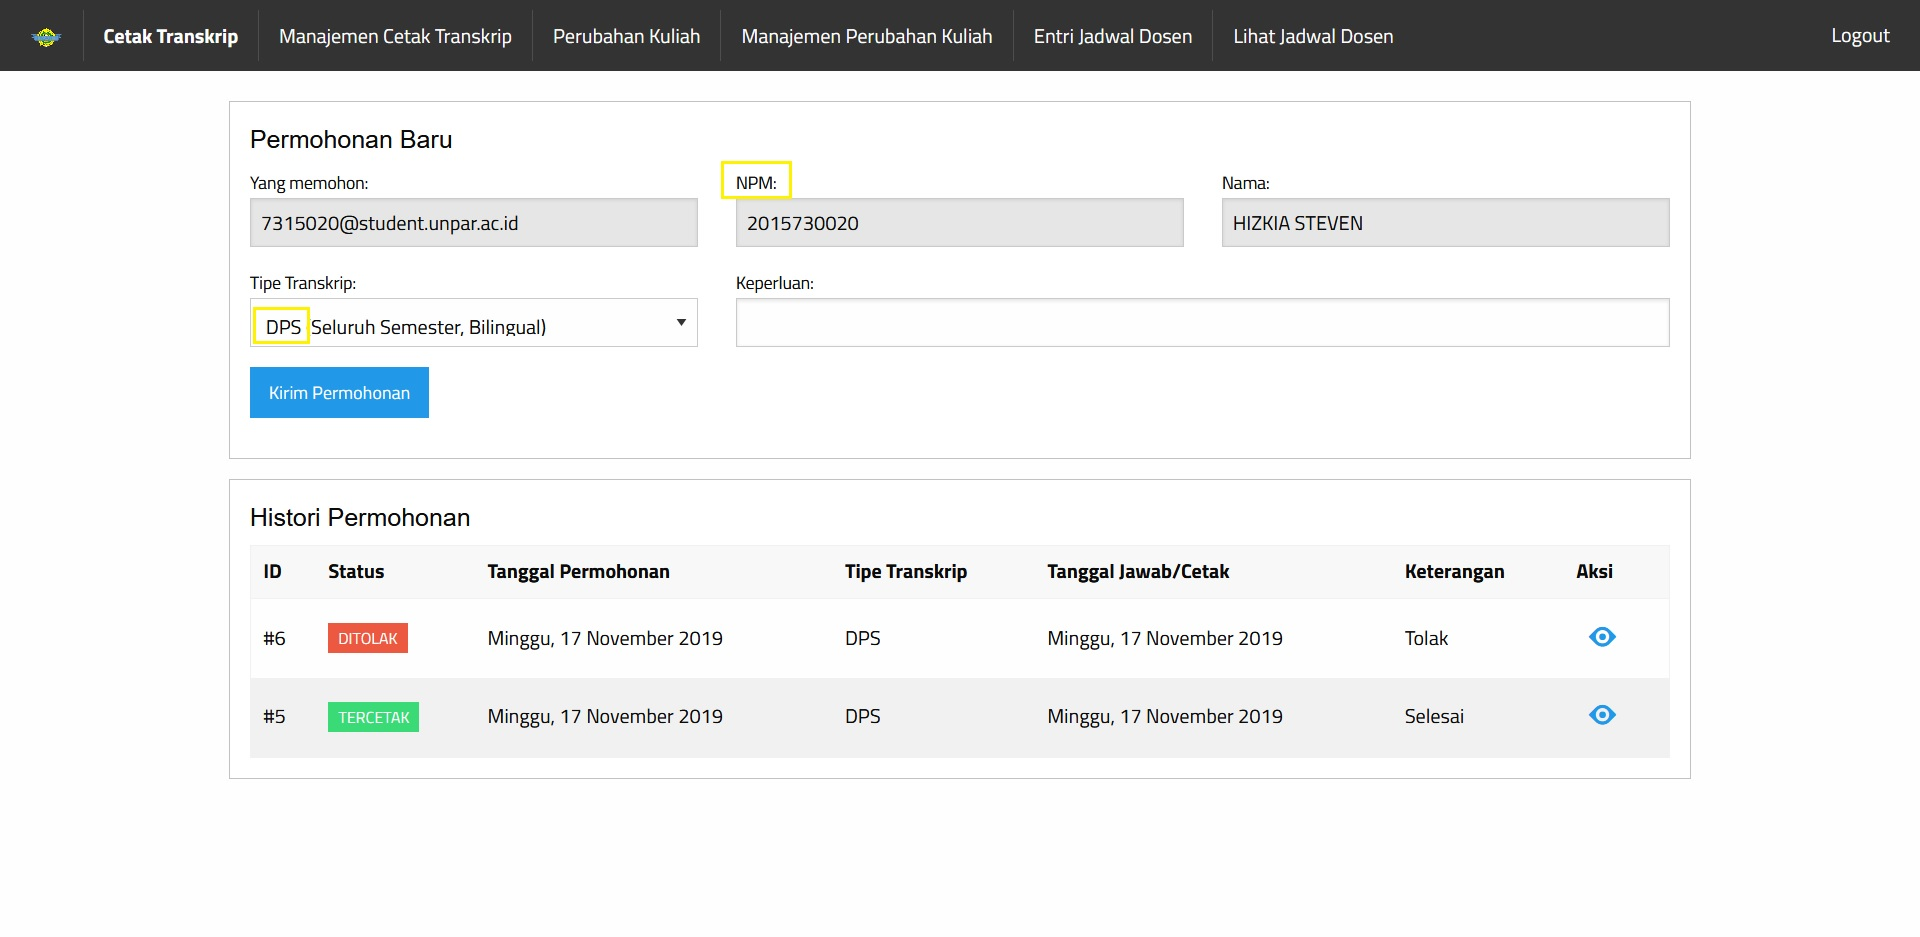
\includegraphics[scale=0.4, frame]{kriteria-sukses-3-1-4-abbreviations-1}  
        \caption[Pelanggaran Kriteria Sukses 3.1.4 pada Halaman Cetak Transkrip]{Pelanggaran Kriteria Sukses 3.1.4 pada Halaman Cetak Transkrip}
        \label{fig:3.1.4_abbreviations_1}  
    \end{figure}

    \item Pada halaman manajemen cetak transkrip terdapat singkatan "NPM". Letak kesalahan dapat dilihat pada \textit{Listing} \ref{lst:3.1.4_singkatan_pada_halaman_manajemen_cetak_transkrip}. Contoh tampilan pada halaman web dapat dilihat pada Gambar \ref{fig:3.1.4_abbreviations_2}. Tautan untuk halaman yang bermasalah dapat dilihat di \url{https://bluetape.azurewebsites.net/TranskripManage}.
    \begin{lstlisting}[frame=single, label={lst:3.1.4_singkatan_pada_halaman_manajemen_cetak_transkrip}, language=HTML, caption=Pelanggaran Kriteria Sukses 3.1.4 pada Halaman Manajemen Cetak Transkrip]
        <div class="input-group">
            <span class="input-group-label">Cari NPM:</span>
            <input name="npm" class="input-group-field" type="text" placeholder="2013730013" maxlength="10" minlength="10"/>
    \end{lstlisting}

    \begin{figure}[H]
        \centering  
        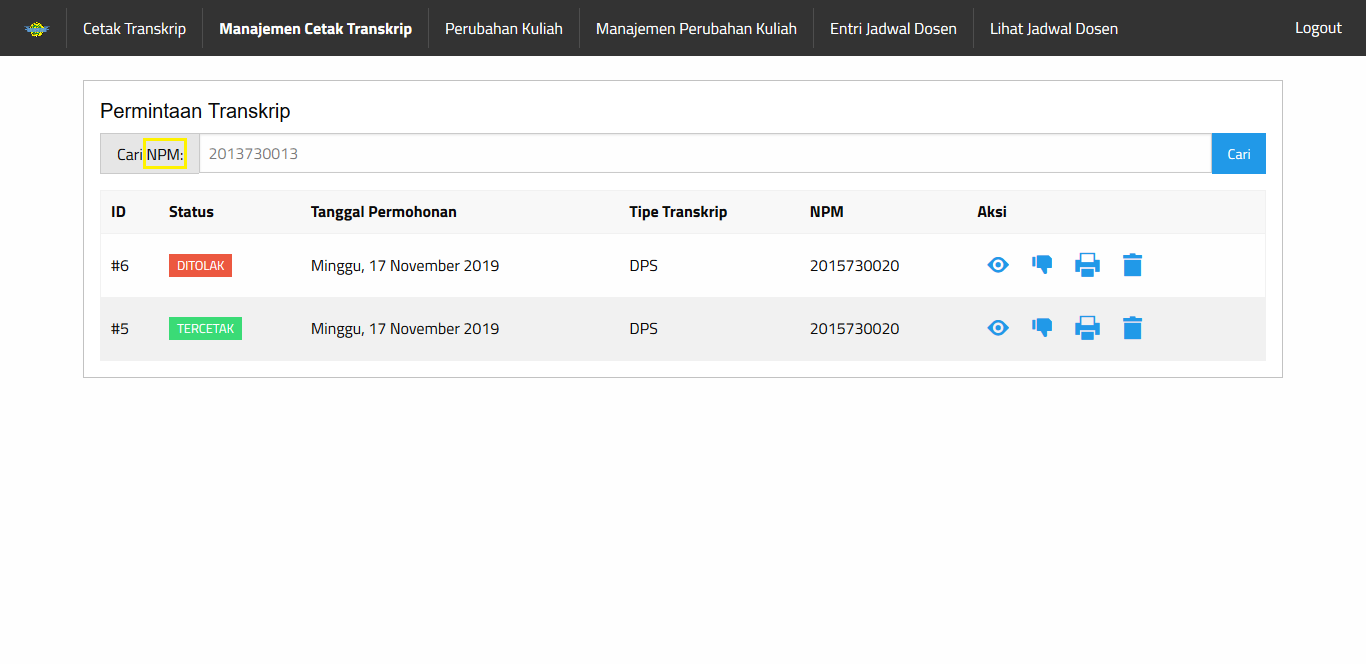
\includegraphics[scale=0.4, frame]{kriteria-sukses-3-1-4-abbreviations-2}  
        \caption[Pelanggaran Kriteria Sukses 3.1.4 pada Halaman Manajemen Cetak Transkrip]{Pelanggaran Kriteria Sukses 3.1.4 pada Halaman Manajemen Cetak Transkrip}
        \label{fig:3.1.4_abbreviations_2}  
    \end{figure}
    
    \item Pada halaman perubahan kuliah terdapat singkatan "MK". Letak kesalahan dapat dilihat pada \textit{Listing} \ref{lst:3.1.4_singkatan_pada_halaman_perubahan_kuliah}. Contoh tampilan pada halaman web dapat dilihat pada Gambar \ref{fig:3.1.4_abbreviations_3}. Tautan untuk halaman yang bermasalah dapat dilihat di \url{https://bluetape.azurewebsites.net/PerubahanKuliahRequest}.
    \begin{lstlisting}[frame=single, label={lst:3.1.4_singkatan_pada_halaman_perubahan_kuliah}, language=HTML, caption=Pelanggaran Kriteria Sukses 3.1.4 pada Halaman Perubahan Kuliah]
        <div class="large-2 column">
            <label>Kode MK:
                <input type="text" name="mataKuliahCode" required maxlength="9" pattern="[A-Z]{3}[0-9]{3}([0-9]{3})?" title="Kode MK dalam format XYZ123"/>
    \end{lstlisting}

    \begin{figure}[H]
        \centering  
        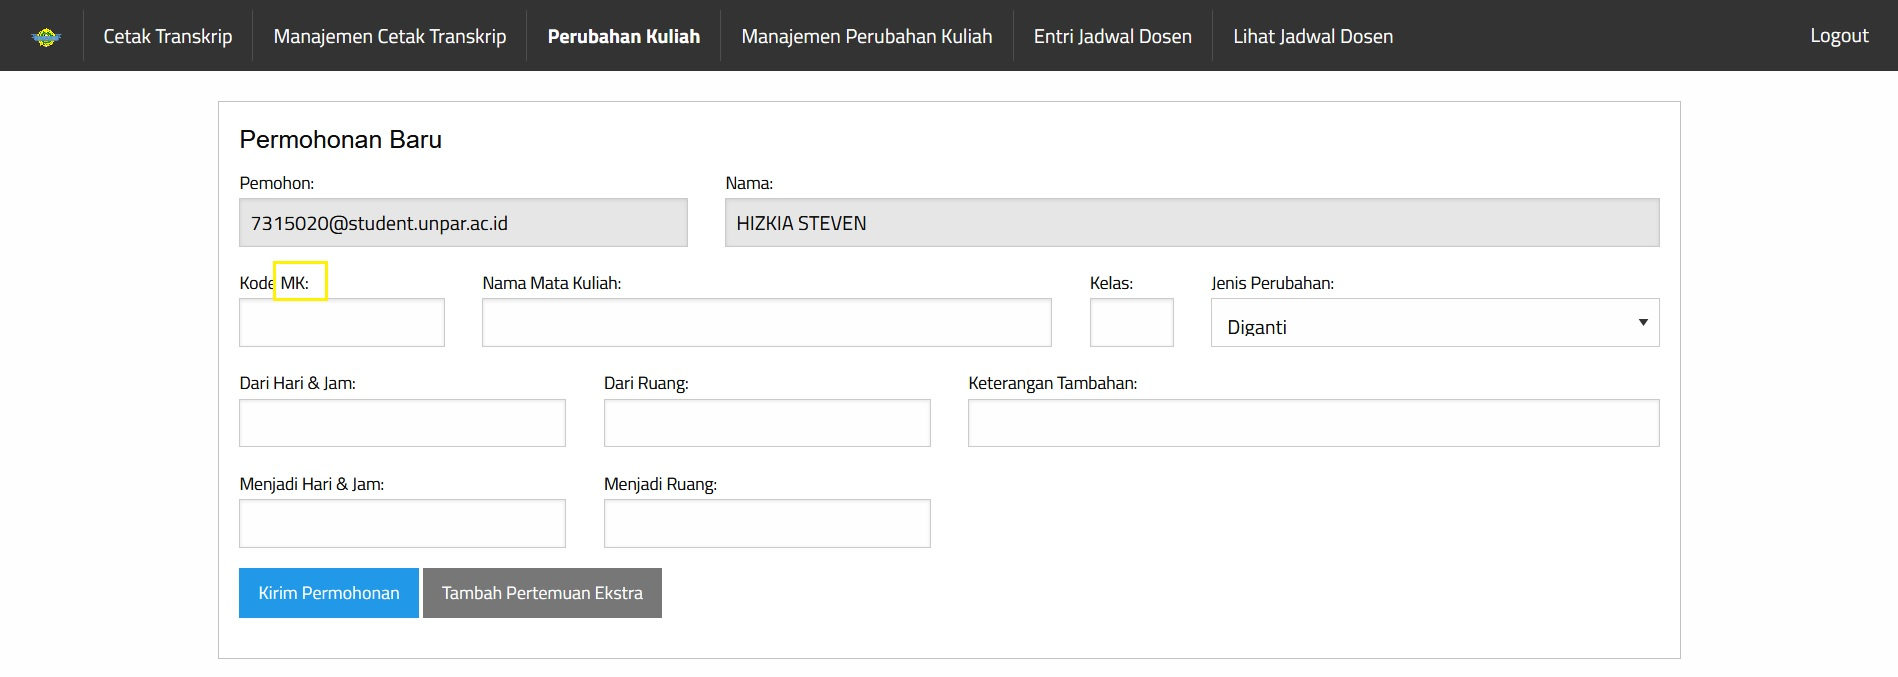
\includegraphics[scale=0.4, frame]{kriteria-sukses-3-1-4-abbreviations-3}  
        \caption[Pelanggaran Kriteria Sukses 3.1.4 pada Halaman Perubahan Kuliah]{Pelanggaran Kriteria Sukses 3.1.4 pada Halaman Perubahan Kuliah}
        \label{fig:3.1.4_abbreviations_3}  
    \end{figure}
    
    \item Pada halaman manajemen perubahan kuliah terdapat singkatan "MK". Letak kesalahan dapat dilihat pada \textit{Listing} \ref{lst:3.1.4_singkatan_pada_halaman_manajemen_perubahan_kuliah}. Contoh tampilan pada halaman web dapat dilihat pada Gambar \ref{fig:3.1.4_abbreviations_4}. Tautan untuk halaman yang bermasalah dapat dilihat di \url{https://bluetape.azurewebsites.net/PerubahanKuliahManage}.
    \begin{lstlisting}[frame=single, label={lst:3.1.4_singkatan_pada_halaman_manajemen_perubahan_kuliah}, language=HTML, caption=Pelanggaran Kriteria Sukses 3.1.4 pada Halaman Manajemen Perubahan Kuliah]
        <th>Tanggal Permohonan</th>
        <th>Kode MK</th>
        <th>Perubahan</th>
    \end{lstlisting}

    \begin{figure}[H]
        \centering  
        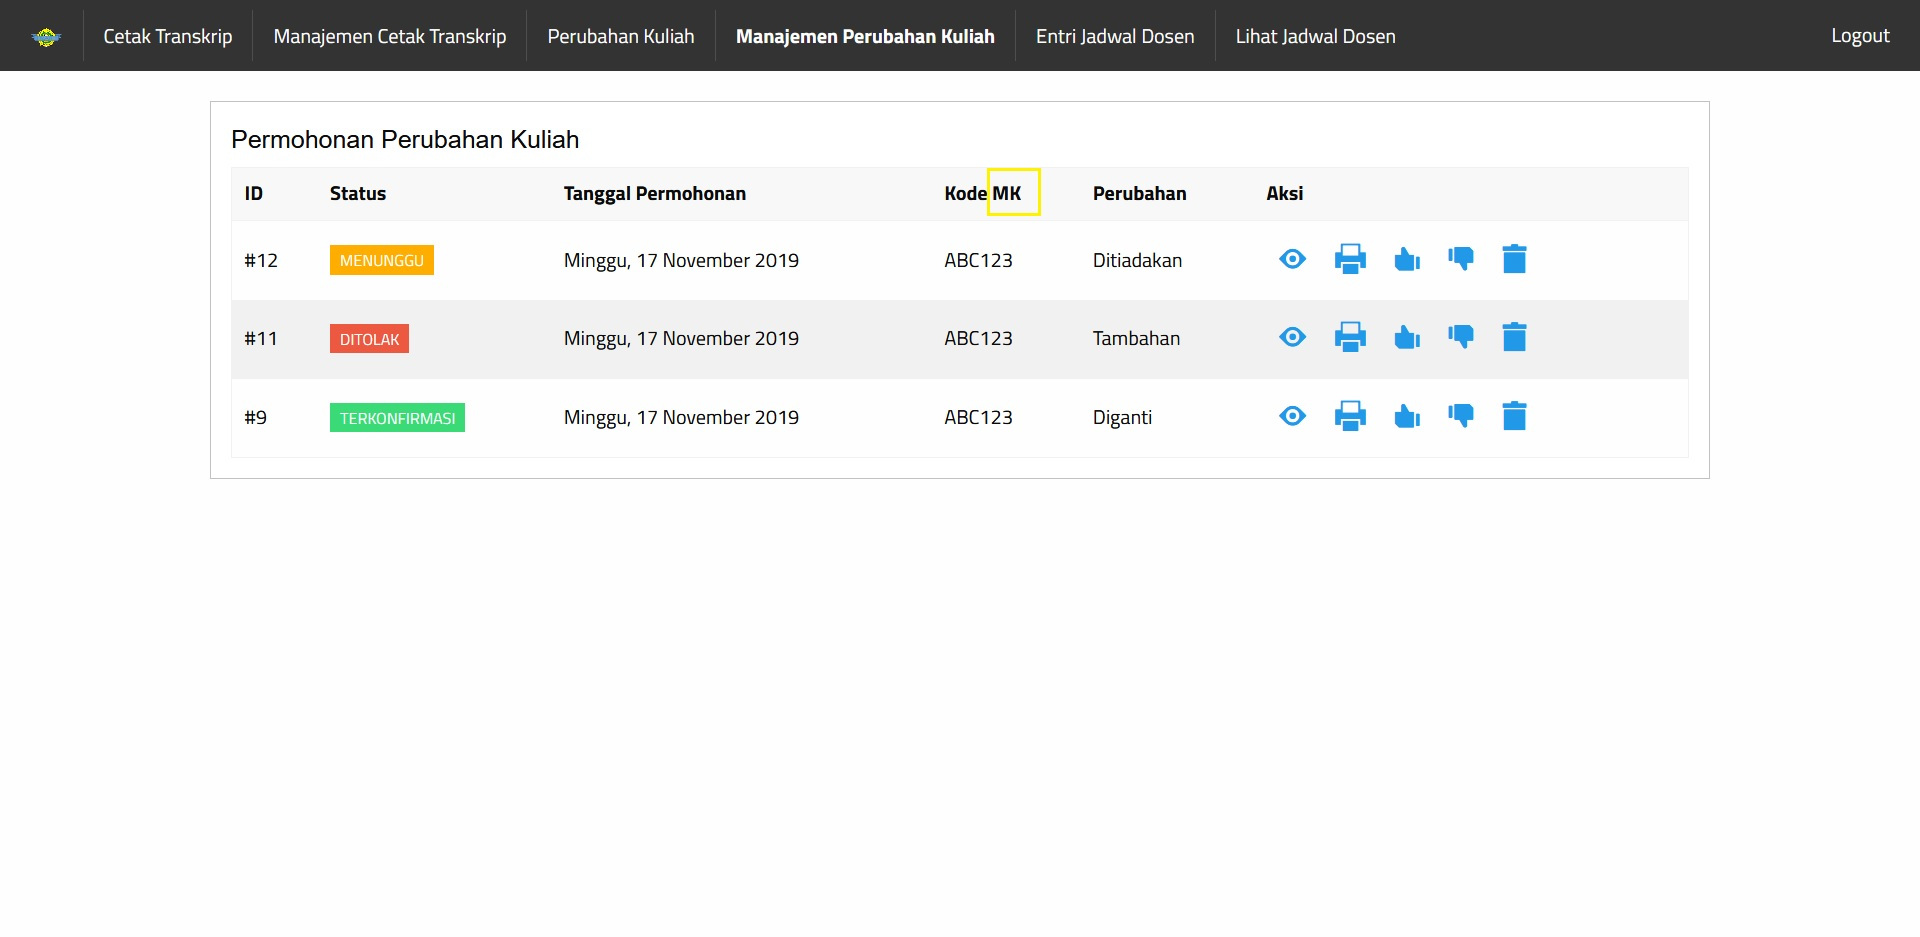
\includegraphics[scale=0.4, frame]{kriteria-sukses-3-1-4-abbreviations-4}  
        \caption[Pelanggaran Kriteria Sukses 3.1.4 pada Halaman Manajemen Perubahan Kuliah]{Pelanggaran Kriteria Sukses 3.1.4 pada Halaman Manajemen Perubahan Kuliah}
        \label{fig:3.1.4_abbreviations_4}  
    \end{figure}
    
    \item Pada halaman entri jadwal dosen terdapat singkatan "XLS". Letak kesalahan dapat dilihat pada \textit{Listing} \ref{lst:3.1.4_singkatan_pada_halaman_entri_jadwal_dosen}. Contoh tampilan pada halaman web dapat dilihat pada Gambar \ref{fig:3.1.4_abbreviations_5}. Tautan untuk halaman yang bermasalah dapat dilihat di \url{https://bluetape.azurewebsites.net/EntriJadwalDosen}.
    \begin{lstlisting}[frame=single, label={lst:3.1.4_singkatan_pada_halaman_entri_jadwal_dosen}, language=HTML, caption=Pelanggaran Kriteria Sukses 3.1.4 pada Halaman Entri Jadwal Dosen]
        <a href="/EntriJadwalDosen/export/" class="button">
            Ekspor ke XLS
        </a>
    \end{lstlisting}

    \begin{figure}[H]
        \centering  
        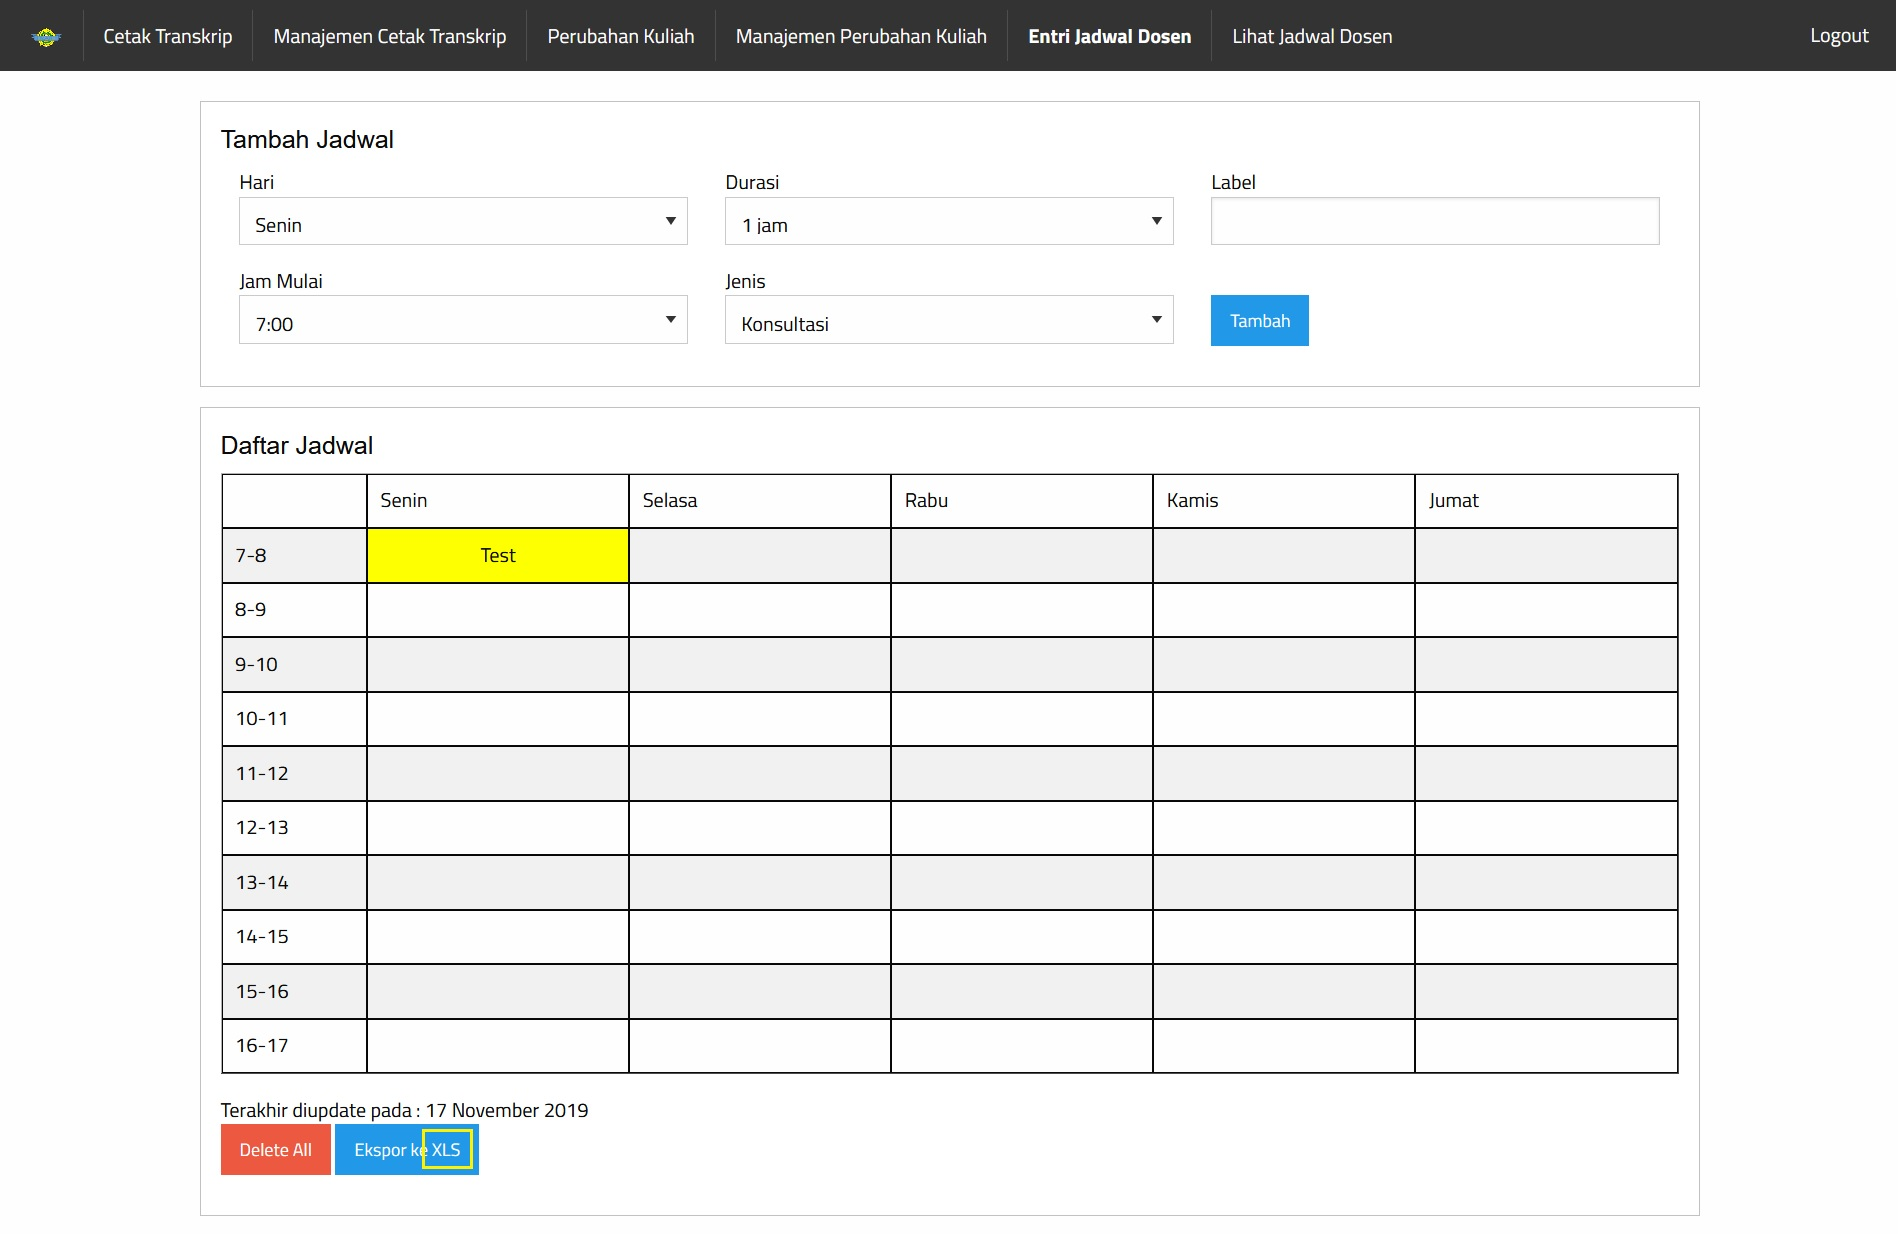
\includegraphics[scale=0.4, frame]{kriteria-sukses-3-1-4-abbreviations-5}  
        \caption[Pelanggaran Kriteria Sukses 3.1.4 pada Halaman Entri Jadwal Dosen]{Pelanggaran Kriteria Sukses 3.1.4 pada Halaman Entri Jadwal Dosen}
        \label{fig:3.1.4_abbreviations_5}  
    \end{figure}
    
    \item Pada halaman lihat jadwal dosen terdapat singkatan "XLS". Letak kesalahan dapat dilihat pada \textit{Listing} \ref{lst:3.1.4_singkatan_pada_halaman_lihat_jadwal_dosen}. Contoh tampilan pada halaman web dapat dilihat pada Gambar \ref{fig:3.1.4_abbreviations_6}. Tautan untuk halaman yang bermasalah dapat dilihat di \url{https://bluetape.azurewebsites.net/LihatJadwalDosen}.
    \begin{lstlisting}[frame=single, label={lst:3.1.4_singkatan_pada_halaman_lihat_jadwal_dosen}, language=HTML, caption=Pelanggaran Kriteria Sukses 3.1.4 pada Halaman Lihat Jadwal Dosen]
        <a href="/LihatJadwalDosen/export/" class="button">
            Ekspor ke XLS
        </a>
    \end{lstlisting}

    \begin{figure}[H]
        \centering  
        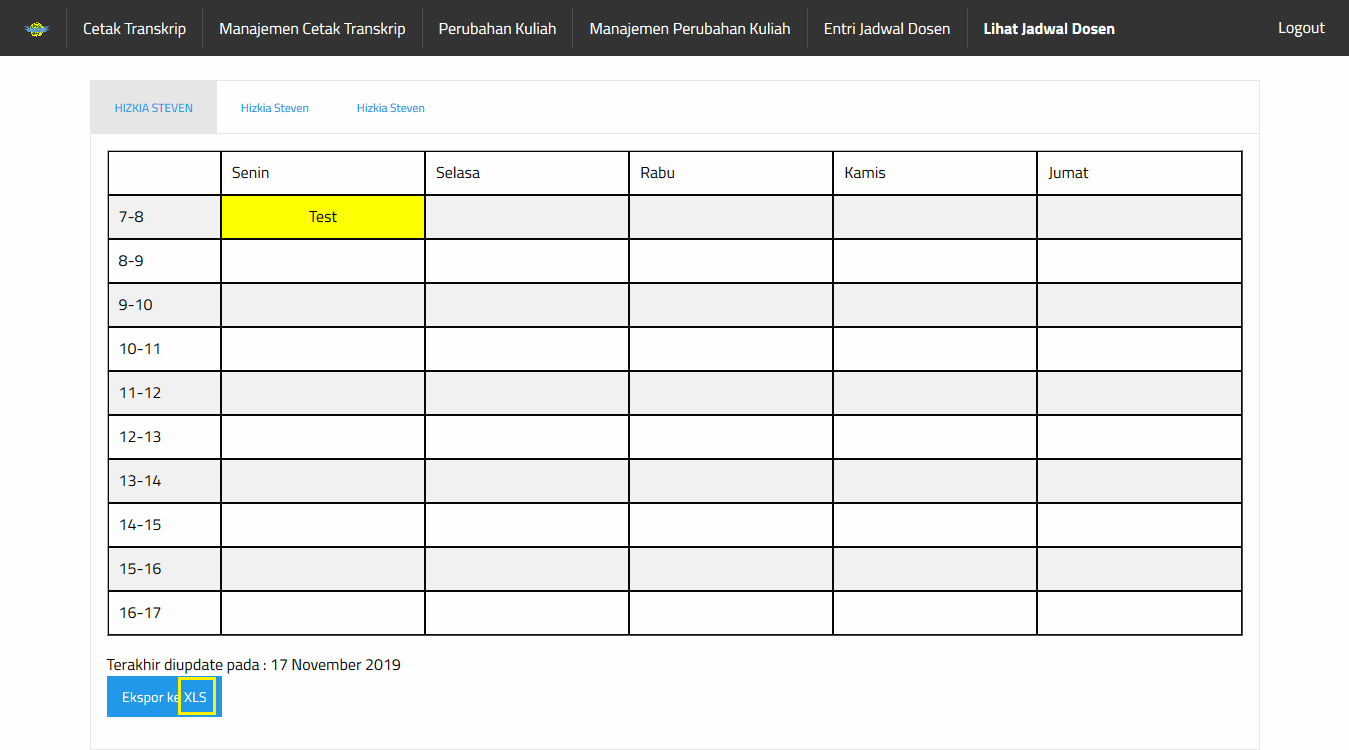
\includegraphics[scale=0.4, frame]{kriteria-sukses-3-1-4-abbreviations-6}  
        \caption[Pelanggaran Kriteria Sukses 3.1.4 pada Halaman Lihat Jadwal Dosen]{Pelanggaran Kriteria Sukses 3.1.4 pada Halaman Lihat Jadwal Dosen}
        \label{fig:3.1.4_abbreviations_6}  
    \end{figure}
\end{itemize}

\paragraph{Kriteria Sukses 3.1.5 \textit{Reading Level}}
\label{par:kepatuhan_bluetape_kriteria_sukses_3.1.5}
(Sukses)\\

Kriteria ini sukses dipatuhi karena pada halaman web BlueTape tidak terdapat teks yang cukup kompleks dan membutuhkan kemampuan membaca yang lebih tinggi dari rata-rata.

\paragraph{Kriteria Sukses 3.1.6 \textit{Pronunciation}}
\label{par:kepatuhan_bluetape_kriteria_sukses_3.1.6}
(Sukses)\\

Kriteria ini sukses dipatuhi karena pada halaman web BlueTape setiap kata dapat dimengerti artinya tanpa pengguna perlu mengetahui cara mengucapkan kata tersebut.

\subsubsection{\textit{Predictable}}
\label{subsubsec:kepatuhan_bluetape_predictable}
Pada subbab ini dibahas alasan mengapa poin kriteria sukses pada kategori \textit{predictable} dinilai sukses atau tidak sukses.

\paragraph{Kriteria Sukses 3.2.1 \textit{On Focus}}
\label{par:kepatuhan_bluetape_kriteria_sukses_3.2.1}
(Sukses)\\

Kriteria ini sukses dipatuhi karena setiap komponen antarmuka pengguna yang menerima fokus, tidak menyebabkan perubahan konteks.

\paragraph{Kriteria Sukses 3.2.2 \textit{On Input}}
\label{par:kepatuhan_bluetape_kriteria_sukses_3.2.2}
(Sukses)\\

Kriteria ini sukses dipatuhi karena ketika pengguna mengubah setelan komponen antarmuka pengguna tidak terjadi perubahan konteks otomatis.

\paragraph{Kriteria Sukses 3.2.3 \textit{Consistent Navigation}}
\label{par:kepatuhan_bluetape_kriteria_sukses_3.2.3}
(Sukses)\\

Kriteria ini sukses dipatuhi karena bagian menu navigasi yang muncul berulang pada tiap halaman web BlueTape, muncul dalam urutan relatif yang sama setiap kali tampak.

\paragraph{Kriteria Sukses 3.2.4 \textit{Consistent Identification}}
\label{par:kepatuhan_bluetape_kriteria_sukses_3.2.4}
(Tidak Sukses)\\

Kriteria ini tidak sukses dipatuhi karena terdapat tombol yang memiliki fungsionalitas yang sama yaitu untuk menghapus namun diidentifikasikan dengan nama yang berbeda. Tombol yang dimaksud adalah tombol "Delete" pada bagian "Edit Jadwal" di halaman entri jadwal dosen. Tombol dengan fungsionalitas yang sama di halaman lain diidentifikasi dengan nama "Hapus". Contoh tampilan pada halaman web dapat dilihat pada Gambar \ref{fig:3.2.4_consistent_identification_1} dan \ref{fig:3.2.4_consistent_identification_2}. Tautan untuk halaman yang bermasalah dapat dilihat di \url{https://bluetape.azurewebsites.net/EntriJadwalDosen}.

\begin{figure}[H]
    \centering  
    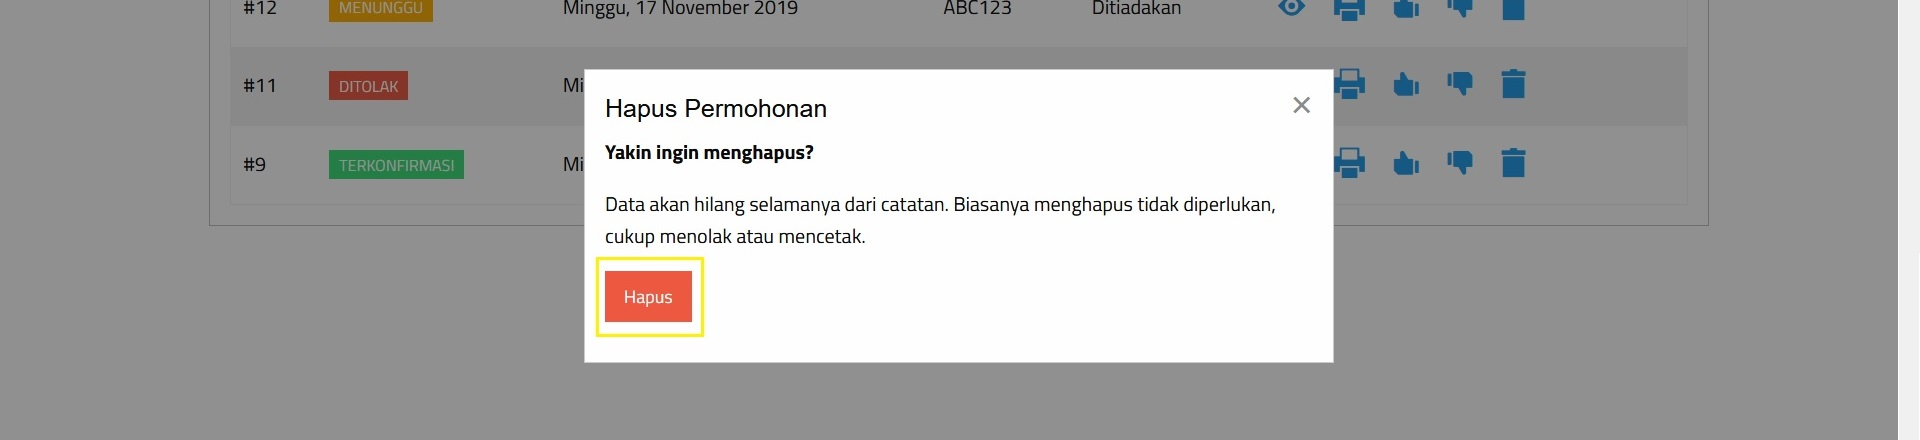
\includegraphics[scale=0.4, frame]{kriteria-sukses-3-2-4-consistent-identification-1-1}  
    \caption[Pelanggaran Kriteria Sukses 3.2.4 pada Kotak Dialog di Halaman Manajemen Perubahan Kuliah]{Pelanggaran Kriteria Sukses 3.2.4 pada Kotak Dialog di Halaman Manajemen Perubahan Kuliah}
    \label{fig:3.2.4_consistent_identification_1}  
\end{figure}

\begin{figure}[H]
    \centering  
    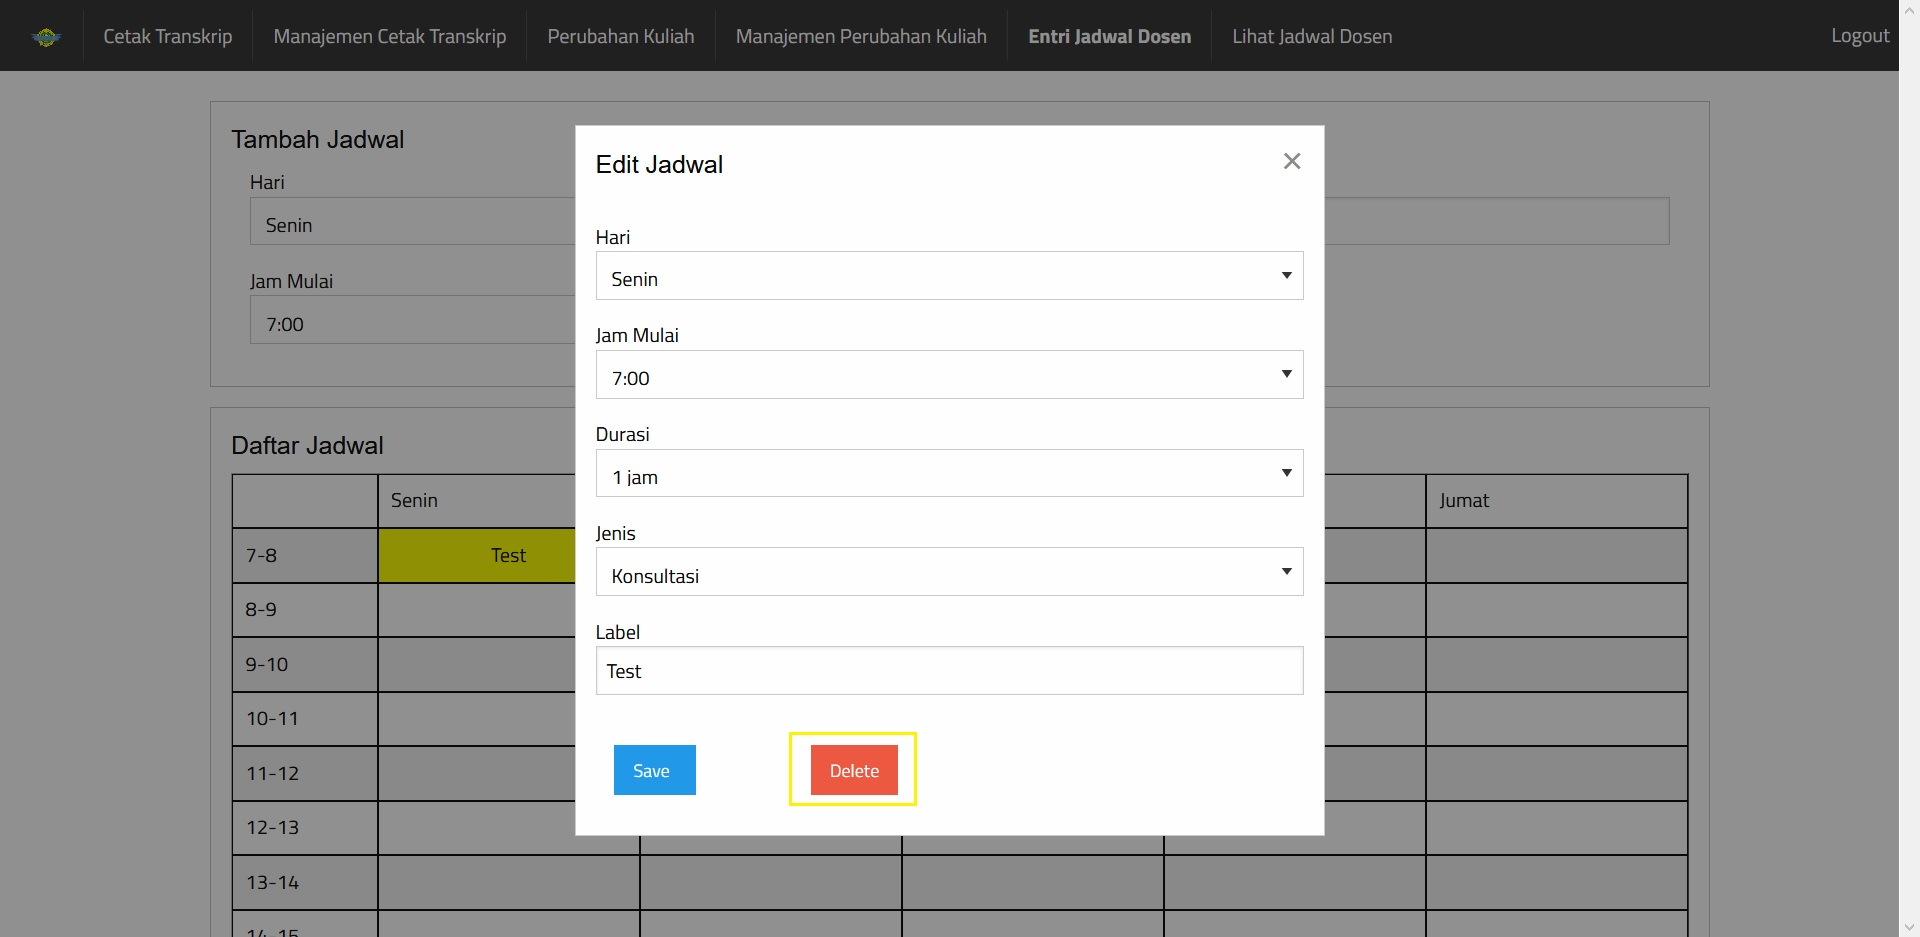
\includegraphics[scale=0.4, frame]{kriteria-sukses-3-2-4-consistent-identification-1-2}  
    \caption[Pelanggaran Kriteria Sukses 3.2.4 pada Kotak Dialog di Halaman Entri Jadwal Dosen]{Pelanggaran Kriteria Sukses 3.2.4 pada Kotak Dialog di Halaman Entri Jadwal Dosen}
    \label{fig:3.2.4_consistent_identification_2}  
\end{figure}

\paragraph{Kriteria Sukses 3.2.5 \textit{Change on Request}}
\label{par:kepatuhan_bluetape_kriteria_sukses_3.2.5}
(Sukses)\\

Kriteria ini sukses dipatuhi karena setiap perubahan konteks hanya terjadi bila dilakukan oleh pengguna.

\subsubsection{\textit{Input Assistance}}
\label{subsubsec:kepatuhan_bluetape_input_assistance}
Pada subbab ini dibahas alasan mengapa poin kriteria sukses pada kategori \textit{input assistance} dinilai sukses atau tidak sukses.

\paragraph{Kriteria Sukses 3.3.1 \textit{Error Identification}}
\label{par:kepatuhan_bluetape_kriteria_sukses_3.3.1}
(Sukses)\\

Kriteria ini sukses dipatuhi karena ketika terdapat kesalahan \textit{input} yang terdeteksi otomatis, bagian yang bermasalah diidentifikasi dan kesalahan dijabarkan kepada pengguna dalam bentuk teks.

\paragraph{Kriteria Sukses 3.3.2 \textit{Labels or Instructions}}
\label{par:kepatuhan_bluetape_kriteria_sukses_3.3.2}
(Tidak Sukses)\\

Kriteria ini tidak sukses dipatuhi karena pada halaman manajemen cetak transkrip dan entri jadwal dosen, setiap elemen \textit{input} tidak memiliki label yang menjelaskan tujuan dari elemen tersebut. Contoh kesalahan dapat dilihat pada \textit{Listing} \ref{lst:3.3.2_label_masukan_entri_jadwal_dosen}. Tautan untuk halaman yang bermasalah dapat dilihat di \url{https://bluetape.azurewebsites.net/EntriJadwalDosen}.

\begin{lstlisting}[frame=single, label={lst:3.3.2_label_masukan_entri_jadwal_dosen}, language=HTML, caption=Pelanggaran Kriteria Sukses 3.3.2 pada Halaman Entri Jadwal Dosen]
    <input type="hidden" name="csrf_token" value="3c159eae7bc953dd591b679c080ed066"/>
    Hari
    <select name="hari">
\end{lstlisting}

\paragraph{Kriteria Sukses 3.3.3 \textit{Error Suggestion}}
\label{par:kepatuhan_bluetape_kriteria_sukses_3.3.3}
(Sukses)\\

Kriteria ini sukses dipatuhi karena ketika terdapat kesalahan \textit{input} yang terdeteksi otomatis, saran untuk mengoreksi kesalahan tersebut disajikan kepada pengguna.

\paragraph{Kriteria Sukses 3.3.4 \textit{Error Prevention (Legal, Financial, Data)}}
\label{par:kepatuhan_bluetape_kriteria_sukses_3.3.4}
(Sukses)\\

Kriteria ini sukses dipatuhi karena pada halaman yang mengirim tanggapan pengguna, data yang dimasukkan oleh pengguna diperiksa terkait kesalahan \textit{input} dan pengguna dipersilakan untuk mengoreksinya.

\paragraph{Kriteria Sukses 3.3.5 \textit{Help}}
\label{par:kepatuhan_bluetape_kriteria_sukses_3.3.5}
(Tidak Sukses)\\

Kriteria ini tidak sukses dipatuhi karena pada halaman entri jadwal dosen, setiap elemen \textit{input} tidak memiliki label yang menjelaskan tujuan dari elemen tersebut. Contoh kesalahan dapat dilihat pada \textit{Listing} \ref{lst:3.3.5_label_masukan_entri_jadwal_dosen}. Tautan untuk halaman yang bermasalah dapat dilihat di \url{https://bluetape.azurewebsites.net/EntriJadwalDosen}.

\begin{lstlisting}[frame=single, label={lst:3.3.5_label_masukan_entri_jadwal_dosen}, language=HTML, caption=Pelanggaran Kriteria Sukses 3.3.5 pada Halaman Entri Jadwal Dosen]
    <input type="hidden" name="csrf_token" value="3c159eae7bc953dd591b679c080ed066"/>
    Hari
    <select name="hari">
\end{lstlisting}

\paragraph{Kriteria Sukses 3.3.6 \textit{Error Prevention (All)}}
\label{par:kepatuhan_bluetape_kriteria_sukses_3.3.6}
(Sukses)\\

Kriteria ini sukses dipatuhi karena pada halaman yang mewajibkan pengguna mengirim informasi, data yang dimasukkan oleh pengguna diperiksa terkait kesalahan \textit{input} dan pengguna dipersilakan untuk mengoreksinya.

\subsection{\textit{Robust}}
\label{subsec:kepatuhan_bluetape_robust}
Pada subbab ini dibahas kriteria-kriteria sukses yang termasuk ke dalam kategori \textit{robust}. Hasil sukses atau tidaknya aplikasi BlueTape terhadap poin-poin kriteria sukses dalam kategori ini ditampilkan pada Tabel \ref{tab:kepatuhan_bluetape_robust}.

\begin{table}[H]
    \centering 
    \caption{Kepatuhan BlueTape terhadap prinsip \textit{Robust}}
    \label{tab:kepatuhan_bluetape_robust}
    \begin{tabular}{|c|c|c|}
        \toprule
        Kriteria Sukses & Hasil (sukses/tidak) & Tingkat Kepatuhan\\

        \midrule
        \rowcolor{darkred} 4.1.1 & Tidak Sukses & A \\
        4.1.2 & Sukses & A \\
        \rowcolor{brightred} 4.1.3 & Tidak Sukses & AA \\

        \bottomrule
        \multicolumn{2}{|c|}{Tingkat kepatuhan tertinggi yang dicapai} & - \\
        \bottomrule

    \end{tabular} 
\end{table}

\subsubsection{\textit{Compatible}}
\label{subsubsec:kepatuhan_bluetape_compatible}
Pada subbab ini dibahas alasan mengapa poin kriteria sukses pada kategori \textit{compatible} dinilai sukses atau tidak sukses.

\paragraph{Kriteria Sukses 4.1.1 \textit{Parsing}}
\label{par:kepatuhan_bluetape_kriteria_sukses_4.1.1}
(Tidak Sukses)\\

Kriteria ini tidak sukses dipatuhi karena terdapat beberapa kesalahan, antara lain:

\begin{itemize}
    \item Pada halaman cetak transkrip, terdapat penggunaan \textit{tag "time"} yang kurang tepat yaitu tidak terdapat \textit{tag} akhir. Letak kesalahan dapat dilihat pada \textit{Listing} \ref{lst:4.1.1_parsing_halaman_cetak_transkrip}. Tautan untuk halaman yang bermasalah dapat dilihat di \url{https://bluetape.azurewebsites.net/TranskripRequest}.
    \begin{lstlisting}[frame=single, label={lst:4.1.1_parsing_halaman_cetak_transkrip}, language=HTML, caption=Pelanggaran Kriteria Sukses 4.1.1 pada Halaman Cetak Transkrip]
        <td>
            <time datetime="2019-11-17 17:55:16">
            Minggu, 17 November 2019
        </td>
    \end{lstlisting}

    \item Pada halaman entri jadwal dosen, terdapat elemen \textit{"HTML"} yang penempatannya tidak tepat yaitu \textit{tag "div"} berada sebelum \textit{tag "body"}. Letak kesalahan dapat dilihat pada \textit{Listing} \ref{lst:4.1.1_parsing_halaman_entri_jadwal_dosen}. Tautan untuk halaman yang bermasalah dapat dilihat di \url{https://bluetape.azurewebsites.net/EntriJadwalDosen}.
    \begin{lstlisting}[frame=single, label={lst:4.1.1_parsing_halaman_entri_jadwal_dosen}, language=HTML, caption=Pelanggaran Kriteria Sukses 4.1.1 pada Halaman Entri Jadwal Dosen]
        </head>
        <div class="row"></div>        
        <body>
    \end{lstlisting}
\end{itemize}

\paragraph{Kriteria Sukses 4.1.2 \textit{Name, Role, Value}}
\label{par:kepatuhan_bluetape_kriteria_sukses_4.1.2}
(Sukses)\\

Kriteria ini sukses dipatuhi karena pada halaman web BlueTape digunakan komponen antarmuka standar dalam bahasa \textit{markup} yaitu \textit{HTML} yang sudah memenuhi standar sukses untuk kriteria ini.

\paragraph{Kriteria Sukses 4.1.3 \textit{Status Messages}}
\label{par:kepatuhan_bluetape_kriteria_sukses_4.1.3}
(Tidak Sukses)\\

Kriteria ini tidak sukses dipatuhi karena setiap pesan status yang ditampilkan kepada pengguna tidak memiliki atribut \textit{"role"} dengan nilai \textit{"alert"} sehingga teknologi alat bantu tidak dapat mengidentifikasi serta menginformasikan pesan tersebut kepada pengguna. Letak kesalahan dapat dilihat pada \textit{Listing} \ref{lst:4.1.3_pesan_status}.

\begin{lstlisting}[frame=single, label={lst:4.1.3_pesan_status}, language=PHP, caption=Pelanggaran Kriteria Sukses 4.1.3 pada Bagian Pesan Status]
    <?php if (isset($_SESSION['error'])): ?>
        <div class="callout alert"><?= $_SESSION['error'] ?></div>
    <?php endif; ?>
    <?php if (isset($_SESSION['info'])): ?>
        <div class="callout primary"><?= $_SESSION['info'] ?></div>
    <?php endif; ?>
\end{lstlisting}

\section{Peningkatan Poin-Poin yang Tidak Sukses Dipatuhi untuk Kriteria Sukses A}
\label{sec:peningkatan_kriteria_sukses_a}
Pada subbab ini dibahas secara singkat cara untuk membuat kriteria sukses A pada subbab \ref{sec:kepatuhan_bluetape_terhadap_wcag_2.1} yang belum sukses dipatuhi menjadi sukses dipatuhi.

\subsection{Peningkatan Kriteria Sukses 1.1.1 \textit{Non-text Content}}
\label{subsec:peningkatan_kriteria_sukses_1.1.1}
Masalah pada poin ini dapat diperbaiki dengan cara sebagai berikut: 

\begin{itemize}
    \item Pada tombol menu yang tidak memiliki nama diberikan atribut \textit{aria-label} yang diisi dengan nilai "Tombol Menu". Penambahan atribut \textit{aria-label} akan membuat tombol tersebut dapat diidentifikasi oleh teknologi alat bantu.
    \item Pada konten berupa ikon yang tidak memiliki nama diberikan atribut \textit{aria-label} yang diisi dengan nilai yang sesuai dengan fungsi setiap konten ikon.
\end{itemize}

\subsection{Peningkatan Kriteria Sukses 1.3.1 \textit{Info and Relationships}}
\label{subsec:peningkatan_kriteria_sukses_1.3.1}
Masalah pada poin ini dapat diperbaiki dengan cara sebagai berikut:

\begin{itemize}
    \item Pada penggunaan \textit{tag heading} yang tidak tepat, \textit{tag heading} dapat diubah menjadi berurutan dimulai dari \texttt{<h1>} hingga \texttt{<h6>}.
    \item Pada halaman manajemen cetak transkrip, kolom \textit{input} NPM diberi atribut \textit{id} yang diisi dengan nilai "NPM" lalu label "Cari NPM" diubah dari \texttt{<span>} menjadi \texttt{<label>} dan dihubungkan dengan kolom \textit{input} NPM.
    \item Pada halaman entri jadwal dosen, setiap kolom \textit{input} diberi atribut \textit{id} lalu setiap judul kolom dibuat sebagai label dengan menggunakan \textit{tag label} dan dihubungkan dengan kolom \textit{input} yang bersangkutan.
\end{itemize}

\subsection{Peningkatan Kriteria Sukses 2.1.1 \textit{Keyboard}}
\label{subsec:peningkatan_kriteria_sukses_2.1.1}
Masalah pada poin ini dapat diperbaiki dengan cara sebagai berikut:

\begin{itemize}
    \item Pada bagian menu navigasi, atribut \textit{data-responsive-menu="dropdown"} dihilangkan karena isi dari elemen yang mengandung atribut tersebut bukanlah sebuah menu \textit{dropdown}.
    \item Pada bagian tabel "Daftar Jadwal" di halaman entri jadwal dosen, setiap \textit{cell} dalam tabel yang berisi jadwal dosen diberi atribut \textit{tabindex} yang diisi dengan nilai nol. Selanjutnya dibuat kode \textit{JavaScript} untuk memicu aksi membuka kotak dialog ketika tombol "Enter" ditekan pada \textit{cell} yang berisi jadwal dosen.
\end{itemize}

\subsection{Peningkatan Kriteria Sukses 2.4.1 \textit{Bypass Blocks}}
\label{subsec:peningkatan_kriteria_sukses_2.4.1}
Masalah pada poin ini dapat diperbaiki dengan cara membuat mekanisme untuk melompati bagian menu navigasi ketika pengguna sedang bernavigasi menggunakan \textit{keyboard}. Dengan cara ini pengguna dapat langsung menuju ke area utama konten tanpa perlu berulang kali melewati bagian menu navigasi.

\subsection{Peningkatan Kriteria Sukses 2.4.4 \textit{Link Purpose (In Context)}}
\label{subsec:peningkatan_kriteria_sukses_2.4.4}
Masalah pada poin ini dapat diperbaiki dengan cara menambahkan atribut \textit{aria-label} yang diisi dengan nilai yang sesuai dengan fungsi setiap tautan.

\subsection{Peningkatan Kriteria Sukses 2.5.3 \textit{Label in Name}}
\label{subsec:peningkatan_kriteria_sukses_2.5.3}
Masalah pada poin ini dapat diperbaiki dengan cara menambahkan atribut \textit{id} pada setiap kolom \textit{input} lalu setiap judul kolom dibuat sebagai label dengan menggunakan \textit{tag label} dan dihubungkan dengan kolom \textit{input} yang bersangkutan.

\subsection{Peningkatan Kriteria Sukses 3.1.1 \textit{Language of Page}}
\label{subsec:peningkatan_kriteria_sukses_3.1.1}
Masalah pada poin ini dapat diperbaiki dengan cara mengganti setelan bahasa manusia \textit{default} dari bahasa Inggris menjadi bahasa Indonesia.

\subsection{Peningkatan Kriteria Sukses 3.3.2 \textit{Labels or Instructions}}
\label{subsec:peningkatan_kriteria_sukses_3.3.2}
Masalah pada poin ini dapat diperbaiki dengan cara menambahkan atribut \textit{id} pada setiap kolom \textit{input} lalu setiap judul kolom dibuat sebagai label dengan menggunakan \textit{tag label} dan dihubungkan dengan kolom \textit{input} yang bersangkutan.

\subsection{Peningkatan Kriteria Sukses 4.1.1 \textit{Parsing}}
\label{subsec:peningkatan_kriteria_sukses_4.1.1}
Masalah pada poin ini dapat diperbaiki dengan cara:

\begin{itemize}
    \item Pada penggunaan \textit{tag "time"} buka yang tidak disertai dengan \textit{tag "time"} tutup di halaman cetak transkrip, bagian yang tidak lengkap cukup ditambahkan \textit{tag "time"} tutup.
    \item Pada penempatan elemen \textit{"HTML"} yang tidak tepat di halaman entri jadwal dosen, \textit{tag "div"} dipindahkan agar berada sesudah \textit{tag "body"}.
\end{itemize}